\chapter{$bbZZ$ Physics Analysis}

In this chapter, we report on a search for the resonant production of the double Higgs boson system. Higgs boson pairs subsequently decay through the $bbZZ$ channel. The final state consists of two b jets, two charged leptons, and two neutrinos ($2 b 2 l 2 \nu$ final state). Analysed data set was collected in 2016 by the CMS experiment in proton-proton collisions  at  13  TeV COM energy, and corresponds to 35.9 fb$^{-1}$ of the integrated luminosity.  

\section{Physics analysis overview}
\label{sec:an_overview}

We search for di-Higgs production through  the  gluon fusion mechanism mediated by two types of possible heavy resonances (separately): a spin-2 Randall-Sundrum (RS1) Kaluza-Klein (KK) graviton and a spin-0 RS1 radion \cite{WED, Xanda}. The width of the graviton and radion is assumed to be negligible with respect to the experimental resolution. We look for decays of WED particles (X) to the $bbZZ$ and $bbWW$ channels with the two b jets, two charged leptons, and two neutrinos final state $X \rightarrow HH \rightarrow bbZZ/bbWW \rightarrow 2 b 2l 2 \nu$. In the above, one of the Higgs bosons decays to a pair of b quarks and the other Higgs boson decays to ZZ or WW system. We consider only leptonic decays of ZZ and WW. Intermediate taus are allowed to decay to daughter muons and electrons.  We explore the invariant masses of WED particles ranging from 250 to 1000  GeV. The result of the measurement is the production cross section of the resonance times the branching fraction of its decay into the aforementioned $2 b 2 l 2 \nu$ final state. 

In this data analysis (later referred to as the analysis), we will describe first the data sets (often referred to as a dataset) and triggers. The measurement uses the DoubleEG and DoubleMuon PDs defined in the previous chapter. These di-electron and di-muon channels are analysed separately and the information is combined in the final result. To select the events with two prompt charged leptons, a set of triggers is applied. To increase the statistics of the measurement and maximise the number of leptons passing the selection, certain complex trigger strategies are employed. 

We continue then with the discussion on the MC simulation of the signal and background processes (later referred to as signal and background). The signal MC samples had to be produced for both graviton and radion particles for 16 mass points from 250 to 1000 GeV to cover the whole search range.  

The description of the physics object reconstruction and event selection is given. Physics objects are constructed using the information from the CMS subsystems and the output of the PF algorithm. Then, based on the final state signature, the events are selected containing corresponding physics objects. The construction of the Higgs and Z boson candidates is discussed at length. The characteristics of signal and background processes are specified and data-MC SFs are discussed.

MVA technique is used to improve signal-background discrimination. We rely on the BDT classifier to reduce the contribution of the background processes in the signal-enriched regions. In all physics measurements, there are sources of the systematic and statistical uncertainties that affect the final results. We discuss all major uncertainties at length and specify the size of the effect of individual types of uncertainties on the final result. 

We present the statistical analysis used to extract the results of the measurements and discuss the CMS statistical package that has been used to extract the final results. Then, we present the results of the measurement and compare them with the theory predictions. Finally, we discuss the ``grand HH combination'' using measurements of all available HH channels.

The material in this chapter follows the description of two articles to which the author contributed directly \cite{bbZZAN, CMS-PAS-HIG-17-032}.

\section{Data analysis strategy}
\label{sec:strategy}
We form the Lorentz energy-momentum vector associated with the double Higgs system. This vector is constructed as the sum  of  the  Lorentz  vectors  of  the  two  leptons,  two  b-jets,  and  the  four-vector  representing neutrinos (\PTslash).  As the z component of the neutrinos? momentum is unknown, we proceed forming a pseudo transverse mass:
$\tilde{M}_T(HH) = \sqrt{E^2 - p_{z}^2}$ (further referred to as transverse mass for brevity), where $E$ and $p_z$ are the energy and the z axis component of the Lorentz energy-momentum vector of the di-Higgs candidate.

The \mTHH distributions are derived for 16 mass and for both spin hypotheses. The \mTHH is constructed using the signal and background simulations. The distributions are produced separately for the signal-enriched (SR) and control regions (CR), which are defined later in this chapter.

To extract the final results, we perform a simultaneous fit of the sum of the signal and background \mTHH distributions in the SR and CRs to the data. The fits are produced for both di-electron and di-muon channels and the results are combined. We obtain 95\% CL upper limits on the HH production cross times the BFs of the subsequent decay to the final state of this measurement. The employed statistical method is based on the $CL_{S}$ asymptotic procedure~\cite{Zech:1988un}.

\section{Data and Triggers}
\label{sec:data_and_triggers}

\subsection{Data}
The search is performed using DoubleMuon and DoubleEG PDs corresponding to an integrated luminosity of 35.9 fb$^{-1}$ recorded by the CMS experiment during Run 2 in 2016. The data were produced in proton-proton collisions at the LHC at 13 TeV COM energy. The data were collected in several data taking periods and approximate values of the integrated luminosity of these periods are given in the Table \ref{tab:datasets}.

\begin{table}[htbp]
\caption{List of used data sets collected by the CMS in 2016. Each era contains a unique letter identifier and also specifies the date when the data processing was done. If the re-processing was run, the name contains the word ending ``v2''. Corresponding integrated luminosities are shown in the second column.
}
\label{tab:datasets}
\begin{center}
\scalebox{0.8}{
\begin{tabular}{|c|c|} \hline%\hline
Dataset       & $\int\mathcal L$ (\fbinv) \\
\hline
%{\texttt Run2016B-03Feb2017-v1}       & \multirow{2}{*}{$\sim$5.9}  \\
{\texttt Run2016B-03Feb2017-v2}       & {$\sim$5.9}  \\
%{\texttt Run2016B-03Feb2017-v2}       &   \\
{\texttt Run2016C-03Feb2017-v1}       & $\sim$2.7 \\
{\texttt Run2016D-03Feb2017-v1}       & $\sim$4.3 \\
{\texttt Run2016E-03Feb2017-v1}       & $\sim$4.1 \\
{\texttt Run2016F-03Feb2017-v1}       & $\sim$3.2 \\
{\texttt Run2016G-03Feb2017-v1}       & $\sim$3.8 \\
{\texttt Run2016H-03Feb2017-v1}       & $\sim$11.8 \\
\hline
Total Luminosity                        & 35.9 \\
\hline%\hline
\end{tabular}
}
\end{center}
\end{table}

\subsection{Triggers\label{sec:triggers}}
%% Because the analysis is performed in the dielectron and dimuon channels, unprescaled dilepton 
%% triggers with the lowest available transverse momentum thresholds are utilized. The triggers at the L1 and
%% HLT level are listed in table ~\\ref{tab:trgs2015}. Dielectron trigger requires the leading electron to pass $23$ GeV $p_{T}$ cut and $12$ GeV $p_{T}$ cut for the subleading electron. Offline cuts are $25$ GeV $p_{T}$ cut and $15$ GeV $p_{T}$ cut correspondinly. Dimuon triggers require the leading muon to pass $17$ GeV $p_{T}$ cut and $8$ GeV $p_{T}$ cut for the subleading muon with the $20$ GeV $p_{T}$ cut and $15$ GeV $p_{T}$ cut for offline selection correspondinly. $\eta$ region in the gap is excluded (1.4442 to 1.566). 

The data events that are used in this measurement are selected with a set of HLT triggers, each requiring the presence of two muons or two electrons in the event. In the di-electron final state, the trigger requires the leading electron to have the $p_T$ above 23 GeV, and the sub-leading electron to have the $p_T$ above 12 GeV. The latter leg corresponds to a relatively low efficiency electron. Since the measurement is focused on ``golden'' electrons coming from on-shell Z boson decays, the offline selection is slightly tighter than the HLT selection and requires the sub-leading electron to have the $p_T$ above 15 GeV.

The final state that contains two prompt muons is selected with the HLT path that is a combination of several HLT paths chained using the logical ``OR'' operation, in other words, the muons are required to pass the selection of at least one of the HLT paths. At the HLT level, the leading and the sub-leading muons have to pass 17 and 8 GeV $p_T$ requirements respectively. The difference among HLT paths has been explained at length in the Section \ref{ch:cms}. The offline analysis increases the $p_T$ threshold values to 20 and 15 GeV correspondingly. For the offline selection, electrons are selected in the range $\eta < $ 2.5 and muons in the range $\eta < $  2.4. For both channels, the $\eta$ region in the gap (1.4442 to 1.566) between the barrel and endcap is excluded.

The same trigger selections are applied to MC simulated events. The efficiencies are then derived for MC and data, and SFs are determined using the TnP procedure discussed in Section \ref{sec:TnP}. Trigger SFs have been computed for each trigger leg separately, since the selection of each leg varies (Fig. ~\ref{fig:trigger_eff_diele}). Following the recommendations from the CMS Muon POG, scale factors have been calculated separately for two data collecting periods: runs B to G (Fig. \ref{fig:trigger_SF_dimu_BCDEFG}, and run H separately (Fig. \ref{fig:trigger_SF_dimu_H}), since the LHC conditions varied significantly for the run H. All eras have slightly different integrated luminosities, see Table \ref{dab:datasets}, so the final SFs are luminosity averaged. Additionally, as was discussed in the chapter on CMS Physics Objects Reconstruction, some triggers did not contain DZ requirement, while others did. Therefore, scale factors of the DZ selection are also measured, see Fig. \ref{fig:trigger_SF_dimu_dZ_H}). Prior to measuring the trigger scale factors, the electrons and muons were required to satisfy ID and ISO selections, more in the subsections \ref{sec:electrons, sec:muons}. 

\begin{figure}[H]
\centering
\subfloat Leg 1
{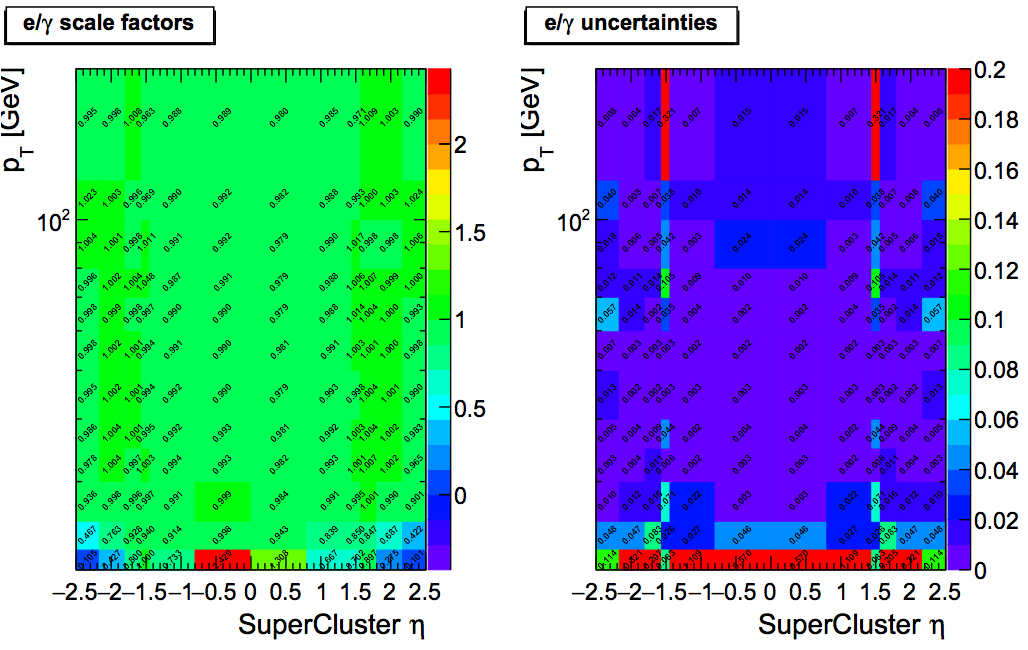
\includegraphics[width=1.0\textwidth]{trigger/electronTriggerEfficiencyelectronTriggerEfficiencyHLT_Leg1_WP90_2016.png} } \\
\subfloat Leg 2
{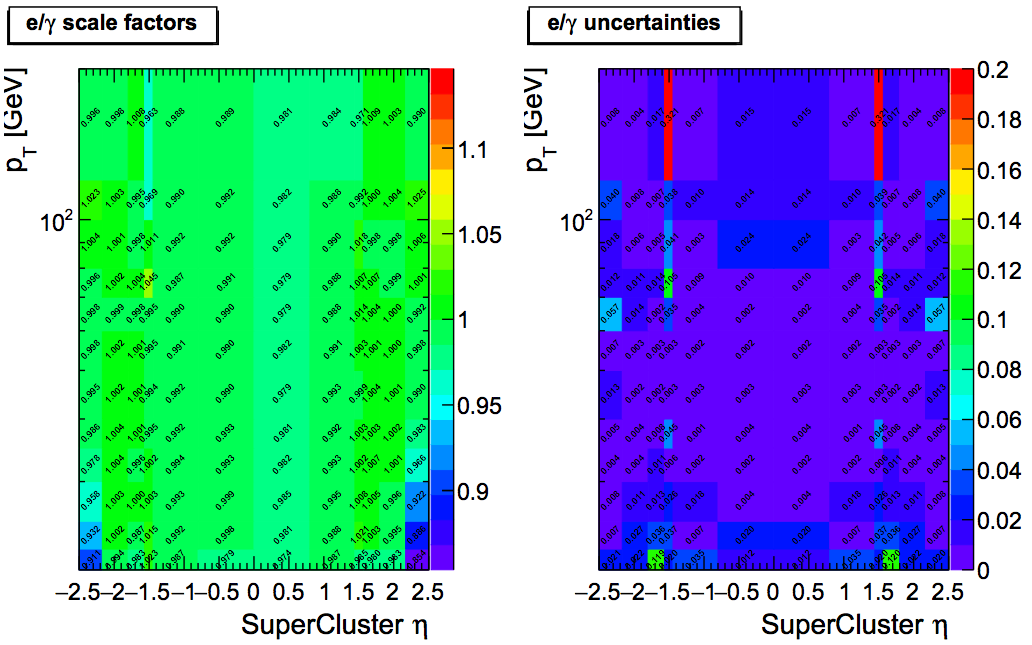
\includegraphics[width=1.0\textwidth]{trigger/electronTriggerEfficiencyelectronTriggerEfficiencyHLT_Leg2_WP90_2016.png} } \\
\caption[HLT trigger SFs for electrons.]{HLT trigger SFs for electrons approved by the CMS $e/ \gamma$ POG group.  SFs are derived for both legs separately: Leg 1 (top) corresponds to the leading electron and Leg 2 (bottom) corresponds to the sub-leading electron. The values of the SFs are shown on the left, and the associated uncertainties with each value are shown on the right. Taken from ~\cite{vhbbAN}.}
\label{fig:trigger_eff_diele}
\end{figure}

\begin{figure}[H]
\centering
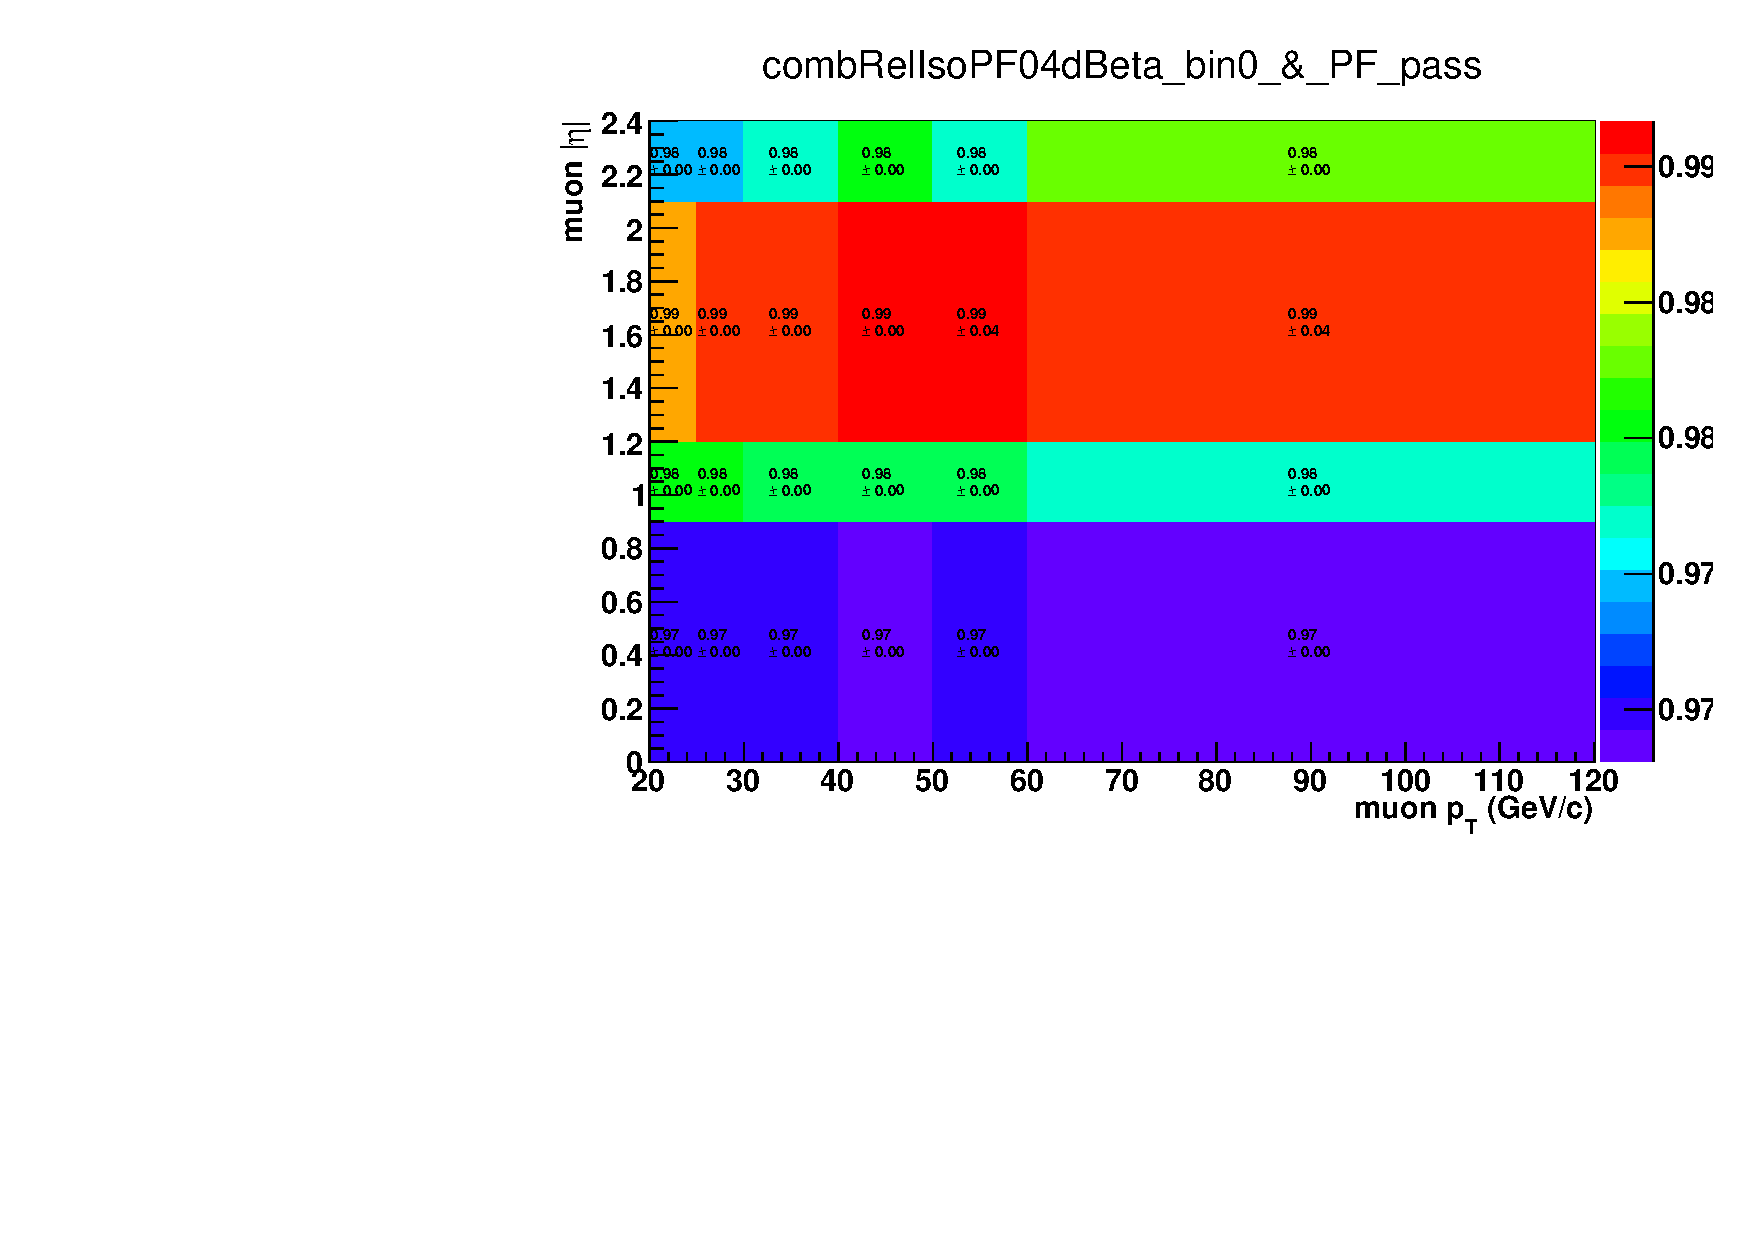
\includegraphics[width=0.475\textwidth]{trigger/Run_BCDEFG_PlotSF_hlt_Mu17_Mu8_OR_TkMu8_leg8_NUM_hlt_Mu17_Mu8_OR_TkMu8_leg8_DEN_LooseIDnISO_PAR_pt_eta_pt_abseta_ratio.pdf}
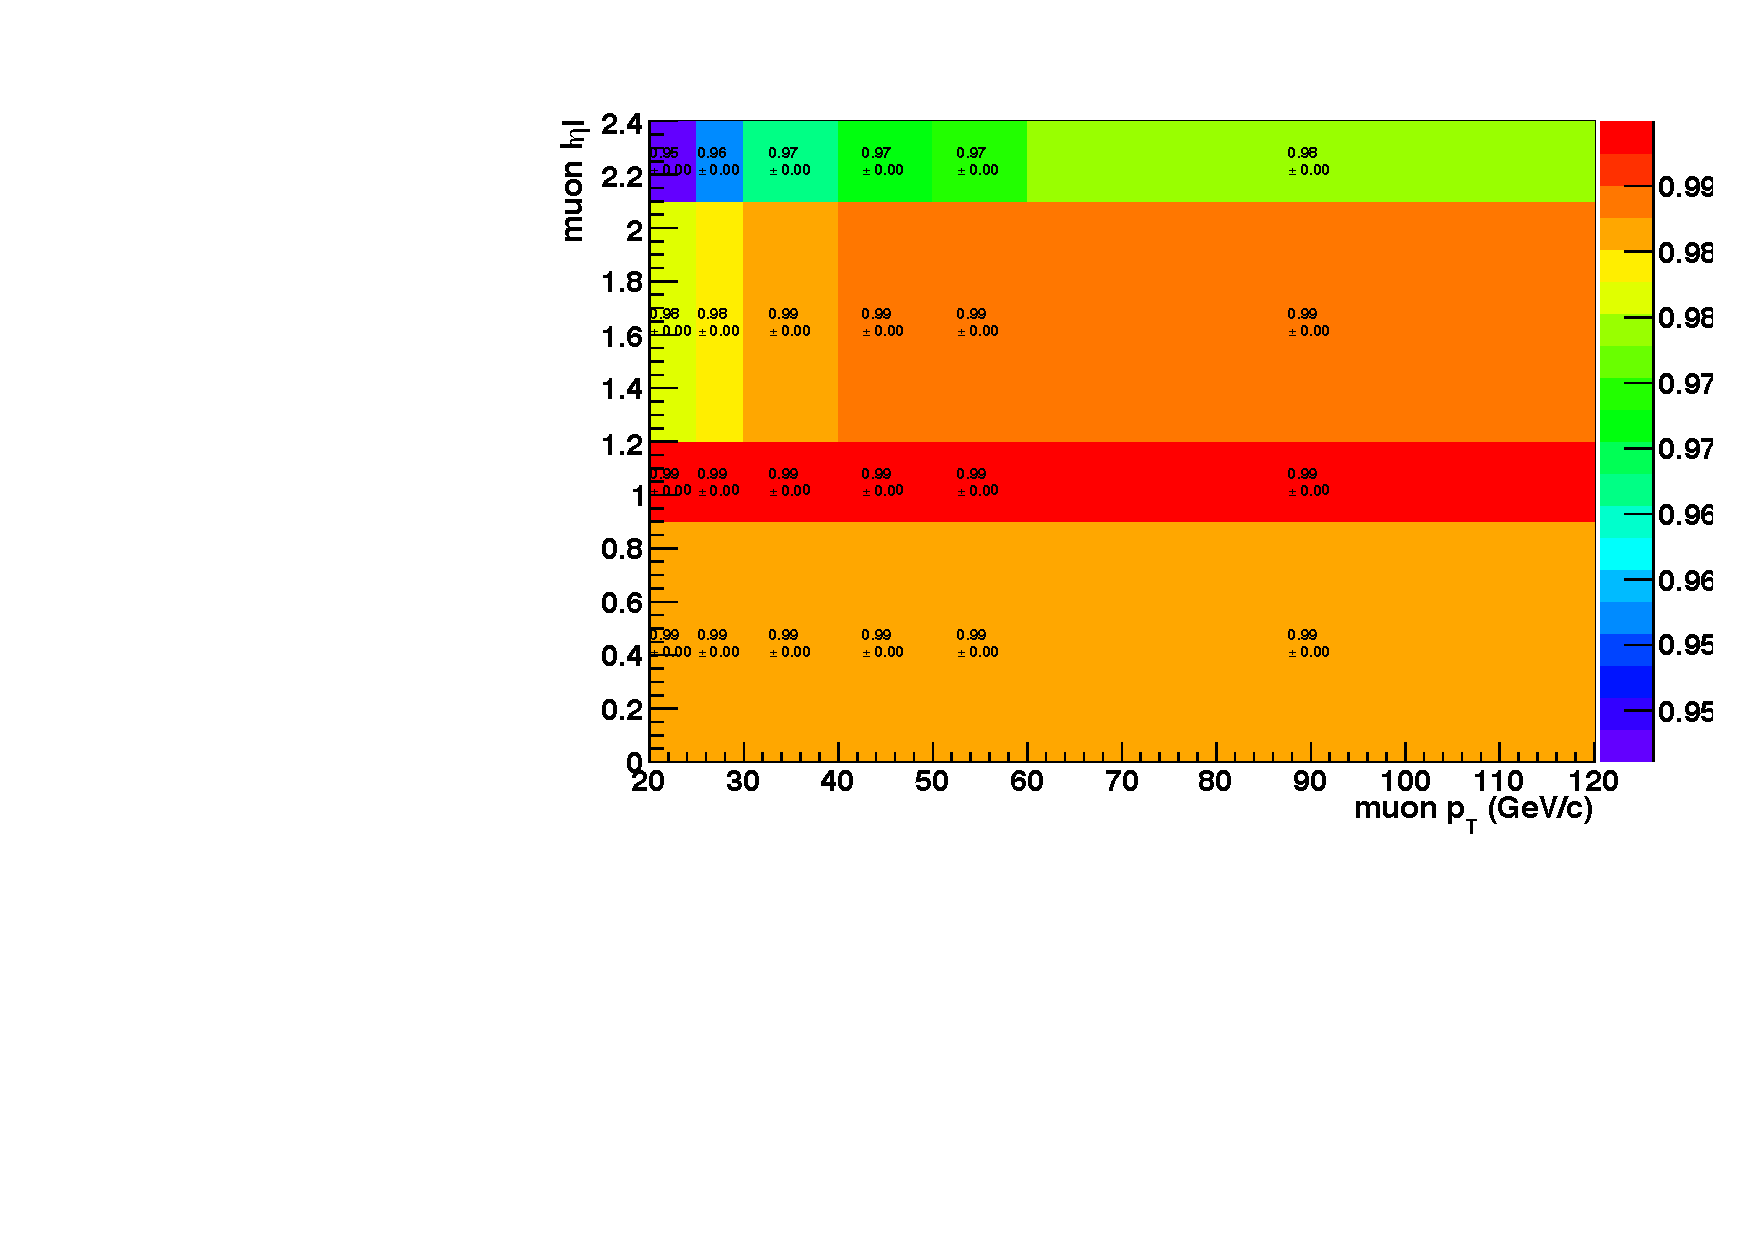
\includegraphics[width=0.475\textwidth]{trigger/Run_BCDEFG_PlotSF_hlt_Mu17Mu8_leg17_NUM_hlt_Mu17Mu8_leg17_DEN_LooseIDnISO_PAR_pt_eta_pt_abseta_ratio.pdf}\\
\caption[Final HLT SFs for muons as a function of $p_{T}$ and $\eta$, measured for eras B to G.]{Final HLT SFs for muons as a function of $p_{T}$ and $\eta$, measured for eras B to G. Left: Scale factors for 8 GeV leg (sub-leading muon). Right: Scale factors for 17 GeV leg (leading muons), provided that the sub-leading muon already passed 8 GeV $p_T$ requirement.}
\label{fig:trigger_SF_dimu_BCDEFG}
\end{figure}

\begin{figure}[H]
\centering
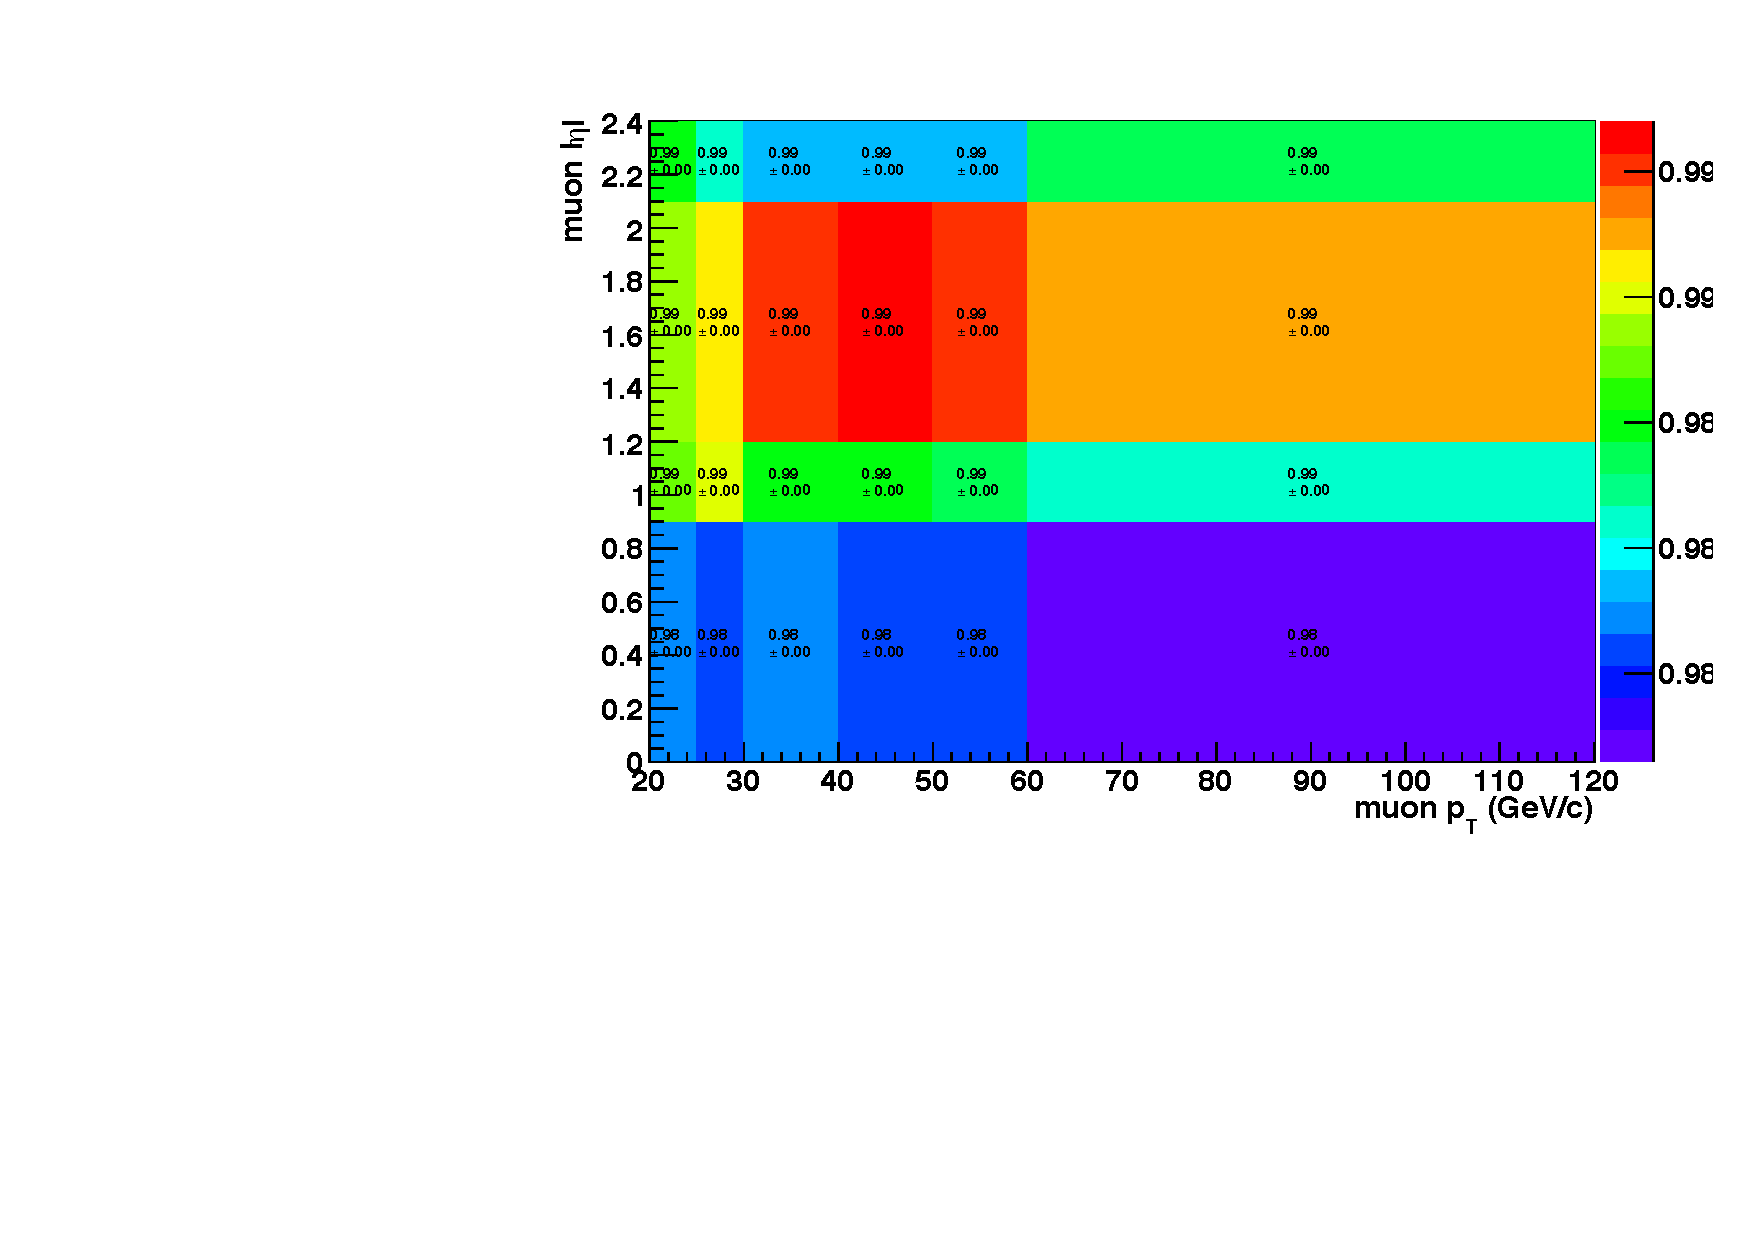
\includegraphics[width=0.475\textwidth]{trigger/Run_H_PlotSF_hlt_Mu17_Mu8_OR_TkMu8_leg8_NUM_hlt_Mu17_Mu8_OR_TkMu8_leg8_DEN_LooseIDnISO_PAR_pt_eta_pt_abseta_ratio.pdf}
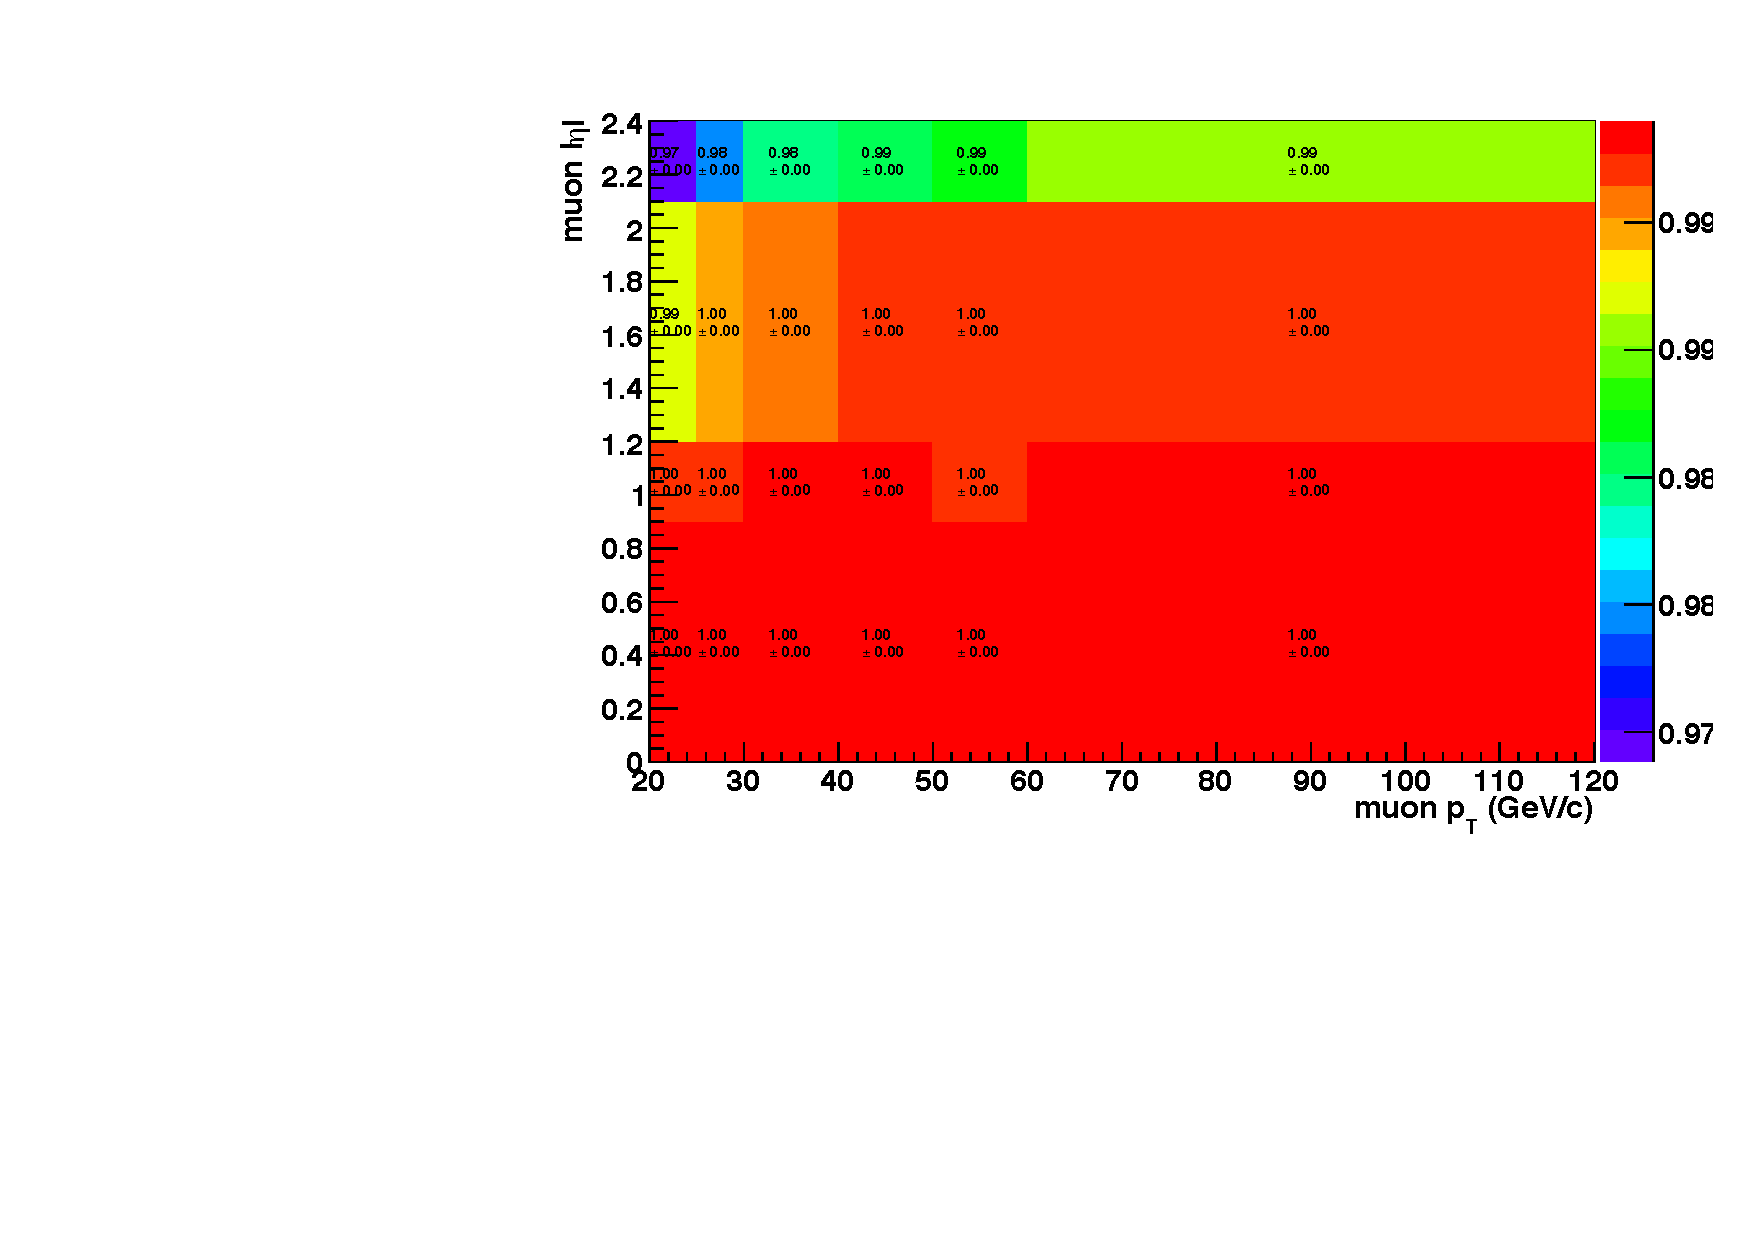
\includegraphics[width=0.475\textwidth]{trigger/Run_H_PlotSF_hlt_Mu17Mu8_leg17_NUM_hlt_Mu17Mu8_leg17_DEN_LooseIDnISO_PAR_pt_eta_pt_abseta_ratio.pdf}\\
\caption[Final HLT SFs for muons as a function of $p_{T}$ and $\eta$, measured for the era H.]{Final HLT SFs for muons as a function of $p_{T}$ and $\eta$, measured for the era H. Left: Scale factors for 8 GeV leg (sub-leading muon). Right: Scale factors for 17 GeV leg (leading muons), provided that the sub-leading muon already passed 8 GeV $p_T$ requirement.}
\label{fig:trigger_SF_dimu_H}
\end{figure}

\begin{figure}[H]
\centering
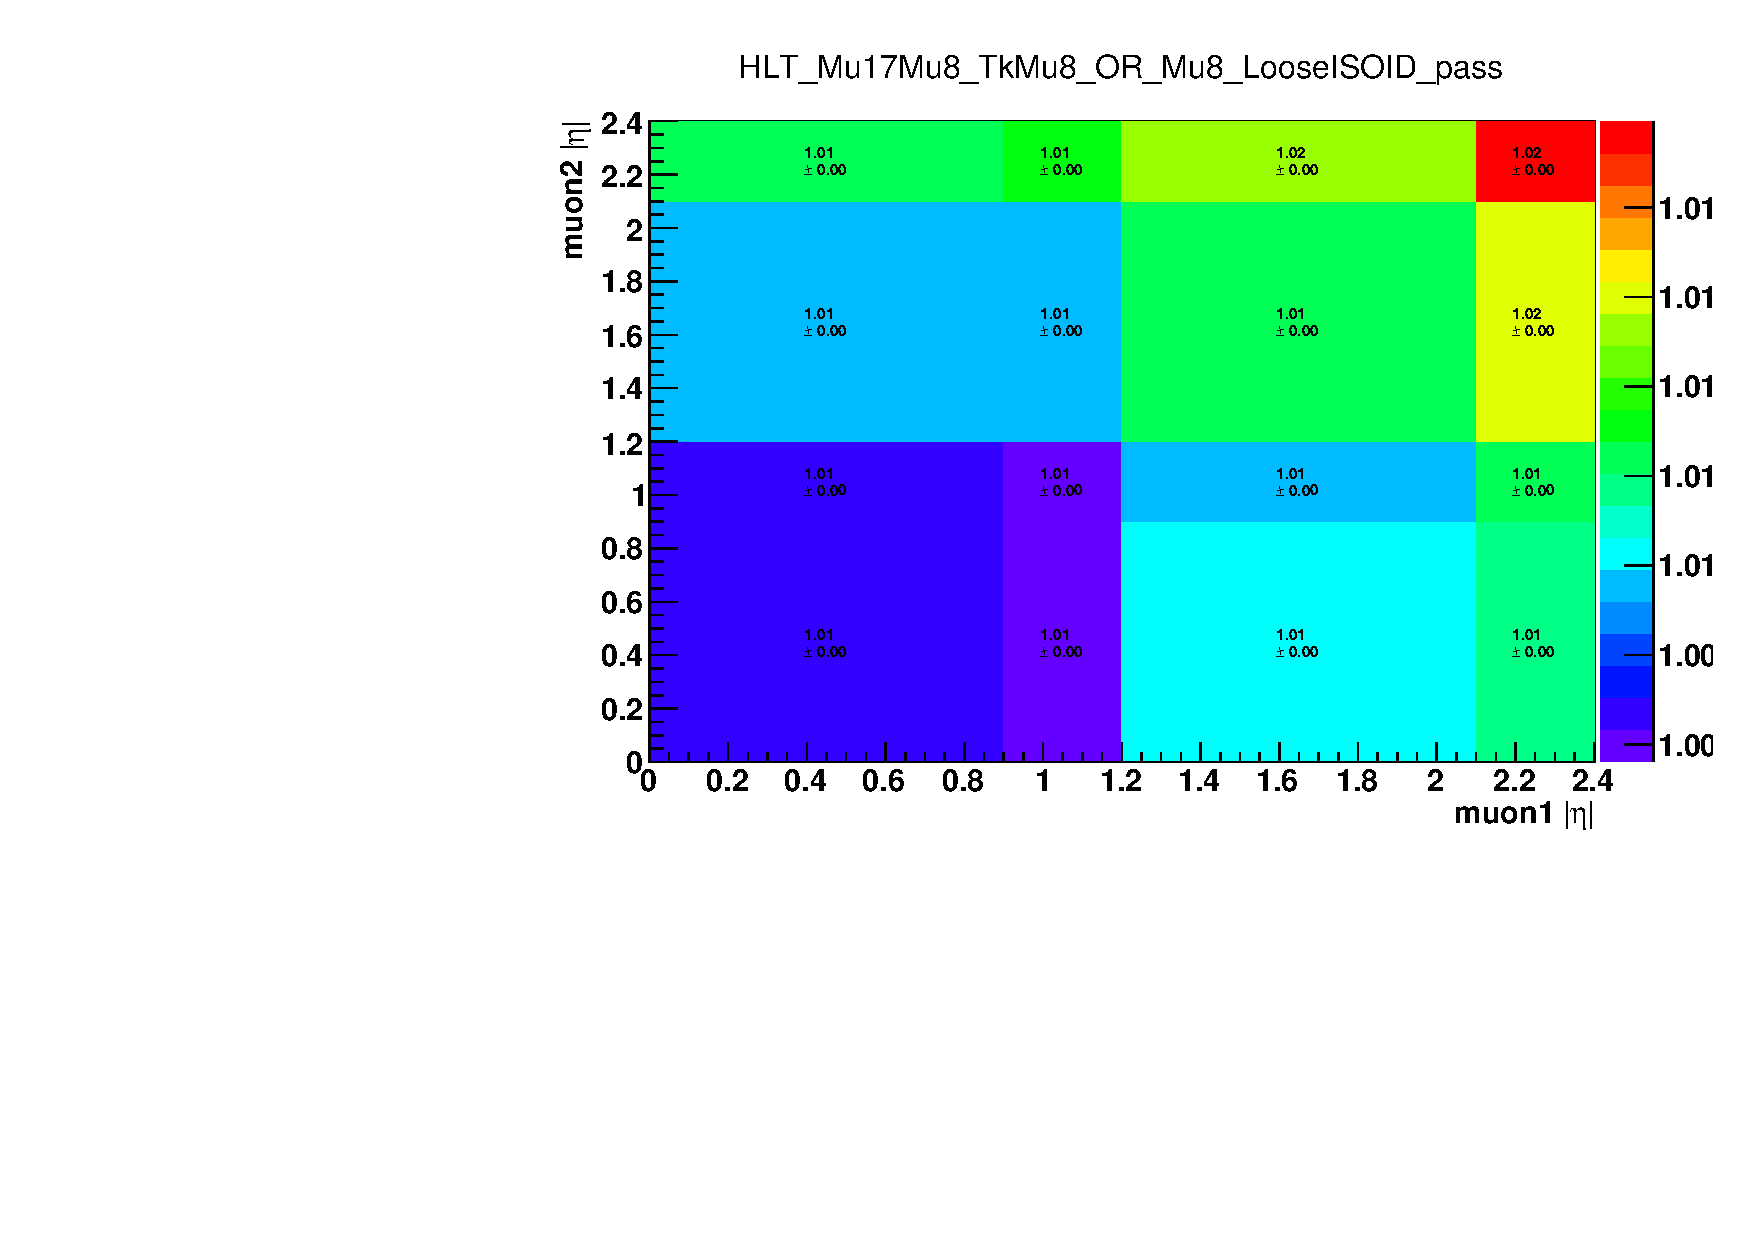
\includegraphics[width=0.85\textwidth]{trigger/PlotSF_dZ_NUM_dZ_DEN_hlt_Mu17_Mu8_OR_TkMu8_loose_PAR_eta1_eta2_abseta_tag_abseta_ratio.pdf}
\caption[SFs for muons of the dZ requirement .]{SFs for muons of the dZ requirement as a function of $\eta$'s of both muons.}
\label{fig:trigger_SF_dimu_dZ_H}
\end{figure}

\section{Simulated Samples}
\label{sec:simulated_samples}
%\section{Monte~Carlo samples\label{sec:mc}}

The data analysis carried out in this thesis is optimised using the MC simulation. MC samples for signal and background processes have been produced with various HEP software (``generators``) that generates the processes of interest: processes that mimic the final state of this measurement. 

\subsection{Signal processes simulation\label{sec:signalMC}}

%
% Signal samples
%
The signal Monte Carlo (MC) samples 
have been generated using {\MGMCatNLO}
%\MGMCatNLO~5 version\ ~2.2.2.0
~\cite{Alwall:2014hca} package. In these samples, simulated at leading
order (LO), gluon fusion production of WED spin-0 and spin-2 narrow resonances is
followed by the decay of the resonances to double Higgs boson system. All Higgs boson are assumed to be SM Higgs bosons with the invariant mass of 125~GeV. Samples are generated for two spin hypotheses and 16 mass values covering the range of heavy resonance masses from 250 to 1000 GeV. Two types of signal samples are present: resonance decaying to $2b 2l 2\nu$ final state through the $X \rightarrow HH \rightarrow bbZZ$ decays and also through the $X \rightarrow HH \rightarrow bbWW$ decays. In both samples the first Higgs boson decays to a pair of \PQb ~quarks. However, in the first sample the other Higgs boson decays to ZZ pair, while 
in the second sample the other Higgs boson decays to WW pair. Only \PZ ~boson decays in the a dielectron,  a dimuon, or a two neutrino state are selected. For \PW ~bosons, the chosen signature is characterised by a W boson decay to an electron and an anti-electron neutrino or a muon accompanied by an anti-muon neutrino.

To compare the expected numbers of events in the simulation to the number of observed events in the data for a given integrated luminosity, the signal production cross section has been normalised to 2 pb. This is a typical value of the production cross section of the WED particle in the 250-300 GeV range, the range to which the current physics analyses are very sensitive with the available LHC data. Additionally, the computed event rates take into account the branching fractions of the corresponding di-Higgs decay chains to the final state: 0.0012 and 0.0266 for $HH\to bbZZ\to bb\ell\ell\nu\nu$ and $HH\to bbWW\to bb\ell\nu\ell\nu$, respectively \cite{CERNYR4}.

%
% Background samples
%

\subsection{Background processes simulation\label{sec:bkgMC}}
In this analysis the main background processes are top-antitop production (\ttbar) and Drell-Yan production in association with jets. 
Other background processes that contribute to a lesser degree include the single top production, diboson production, and the production of a single Higgs boson in association with a Z boson (``ZH production''), see Table \ref{tab:bg_mcsamples}. Other background processes are fully rejected in the event selection and thus are neglected.  

\begin{table}[H]
  %\footnotesize
  %\begin{center}
    \caption{Background Monte Carlo samples\label{tab:bg_mcsamples}
    }
     %\scalebox{0.8}{
    \begin{tabular}{ | l | l | }%|l|r|r|r|r|r|}  % it is separator L separator L separator and all with SPACES
      \hline
      % Sample  & Generator & $m_{H} (\GeV/c^2)$ & $\sigma$ (pb) & events &  $\int\cal L$ (\fbinv) \\
      %\hline
      %\multicolumn{5}{|l|}
      {\texttt{DY plus 1 Jet }} & \MGMCatNLO-PYTHIA \\
%                & \MADGRAPH\,5+\PYTHIA{}\,8 & 725 & 39 800 000 & 54.5 \\
      %\multicolumn{5}{|l|}
      {\texttt{DY plus 2 Jets }} & \MGMCatNLO-PYTHIA \\
%               & \MADGRAPH\,5+\PYTHIA{}\,8 & 725 & 39 800 000 & 54.5 \\
      %\hline
      %\multicolumn{5}{|l|}
      {\texttt{DY plus 3 Jets }} & \MGMCatNLO-PYTHIA \\
%              & \MADGRAPH\,5+\PYTHIA{}\,8 & 394.5 & 19 400 000  & 50.2 \\
      %\hline
      %\multicolumn{5}{|l|}
      {\texttt{DY plus 4 Jets }} & \MGMCatNLO-PYTHIA \\
%             & \MADGRAPH\,5+\PYTHIA{}\,8 & 96.47 & 4 960 000 & 52.2 \\
      %\multicolumn{5}{|l|}
      {\texttt{WW }} & PYTHIA \\
%            & \PYTHIA{}\,8 & 118.7 & 993 640 &  8.37  \\
      %\hline
      %\multicolumn{5}{|l|}
      {\texttt{WZ }} & PYTHIA \\
%           & \PYTHIA{}\,8 & 47.13    &   1 000 000   &   21.22  \\
      %\hline
      %\multicolumn{5}{|l|}
      {\texttt{ZZ }} & PYTHIA \\
%          & \PYTHIA{}\,8 & 16.523     &   985 600   &   59.65  \\
       %\multicolumn{5}{|l|}
       {\texttt{ZH with $H \to b\bar{b}$ and $Z \to \ell \ell$ }} & \MGMCatNLO \\
      %\hline
      %\multicolumn{5}{|l|}
      {\texttt{$t\bar{t}$ }} & POWHEG-PYTHIA \\
       %         & \POWHEG+\PYTHIA{}\,8 & 831.76   & 187 626 200 + 97 994 442&  343  \\
      %\hline
      %\multicolumn{5}{|l|}
      {\texttt{top quark tW channel }} & POWHEG-PYTHIA \\
        %        & \POWHEG+\PYTHIA{}\,8 & 35.6   &   1 000 000   &   28.09  \\
      %\hline
      %\multicolumn{5}{|l|}
      {\texttt{$\bar{t}$ quark tW channel }} & POWHEG-PYTHIA\\
         %       & \POWHEG+\PYTHIA{}\,8 & 35.6   &   999 400   &   28.07  \\
      %\hline\hline
      %\multicolumn{5}{|l|}
      {\texttt{top quark t-channel }} & POWHEG-PYTHIA \\
          %      & \POWHEG+\PYTHIA{}\,8 & 136*0.325   &   999 400   &   22.6 \\
      %\hline
      %\multicolumn{5}{|l|}
      {\texttt{$\bar{t}$ t-channel }} & POWHEG-PYTHIA \\
           %     & \POWHEG+\PYTHIA{}\,8 & 81*0.325   & 1 695 400 &  64.4 \\
      %\hline\hline
      %\multicolumn{5}{|l|}
      {\texttt{top quark s-channel }} & \MGMCatNLO-PYTHIA\\
      %    & \POWHEG+\PYTHIA{}\,8 & 10.32   &   998 400   &   96.74  \\
\hline%\hline
    \end{tabular}
  %\end{center}
  %}
  %\label{backgrounds} 
\end{table}

Drell-Yan (DY) process in association with one to
four jets is generated at leading order (LO) using {\MGMCatNLO} with the MLM
matching scheme~\cite{Alwall:2007fs}. To account for the  higher
order QCD and electroweak effects in V+jets production (following
~\cite{DY_QCDnEWK}), DY events are further reweighted
according to the dilepton transverse momentum. 

The simulations of the background processes associated with top
quark production are generated at next-to-leading order (NLO). 
 {\POWHEG} ~\cite{Alioli:2009je, pwh1, pwh2, pwh3} generator was used to generate the
samples for top quark pair production and single top quark production in the tW
and t channels. For the single top s channel production, the
{\MGMCatNLO} generator was used.  Single top backgrounds have been rescaled to the theoretical values of the NNLO cross sections \cite{Kidonakis:2012db, Czakon:2013goa}. 

{\PYTHIA} 8.212~\cite{Sjostrand:2007gs,Sjostrand:2014zea} was used to generate diboson samples at LO. Diboson
background yields are normalized to NLO cross sections
\cite{CMS-PAS-SMP-18-002, CMS-PAS-SMP-16-006, Khachatryan:2016txa}. The dominant SM Higgs background process, the SM production of a single Higgs boson in the association with a \PZ ~boson (ZH), is simulated
at NLO using the {\MGMCatNLO} generator with FxFx merging ~\cite{Frederix:2012ps}. 
The SM Higgs background from the ZH process is scaled to NNLO with the
MCFM program ~\cite{Campbell:2010ff}. All the final cross section values at the NNLO accuracy in perturbative QCD have been computed with the original generators and are found to be in agreement with the values from the LHC Higgs cross section working group ~\cite{LHCHXSWG, xsecZH, xsecTT, xsecST, xsecVV}.

Normalizations for \ttbar ~and DY
background processes are determined from data, as explained later in this chapter.
%
% General simulation details relevant for all samples 
%
The NNPDF3.0 \cite{Ball:2014uwa} parton distribution functions
(PDF) set is used for all the LO and NLO samples. {\POWHEG} and {\MGMCatNLO} interfaced with
{\PYTHIA}8.212 are used for the parton
showering and hadronization stages. The description of the underlying event is done using 
the tune CUETP8M1 derived in \cite{Khachatryan:2015pea}. For the simulation of the CMS detector response, \GEANTfour~\cite{GEANT4} was used. 
%
% Scale factor corrections
%
For all MC simulations, further reweighting of events is done using the SFs derived to account for 
 the discrepancies between the data and simulation: lepton identification and b tagging efficiencies, see Section \ref{sec:TnP, sec:b_tagging}.
%
% Pileup passage
%
As discussed in the Section \ref{sec:pileup}, multiple overlapping
proton-proton interactions occurred in each bunch crossing during data collecting in 2016, with
an average of 24 hard scattering vertices per event. To account for this fact, all simulated samples include additional interactions
to reproduce the real pileup distribution measured in data.

\section{Physics Objects Selection}
\label{sec:objects}

\hyphenation{fa-shion}
\hyphenation{ener-gy}

During the reconstruction of the collisions at the CMS, data for each event are refined into high-level physics objects that correspond to particles created as a result of the proton-proton interaction. Among the physics objects necessary for this measurements are reconstructed electrons, muons, jets originating from quarks of heavy flavor (b jets), and the missing transverse momentum. The reconstruction details have been given in Section \ref{sec:cms_reco}, here we focus on the analysis specific selection of each of these physics objects.

\subsection{Electrons}\label{sec:electrons}
Electrons are reconstructed using the GSF algorithm \cite{GSF}. The electron candidates are then selected by first applying a loose isolation requirement of 0.4, after which they have to pass Tight ID criteri defined by the CMS $e/\gamma$ POG, see \ref{sec:cms_reco}. At the offline level, the analysis applies additionally the loose WP (WP90)  ~\cite{vhbbAN}. With this WP, utilising variables such as the agreement between the position of the ECAL cluster and GSF track that form the electron, the energy of the 3 by 3 crystal core of the electron?s cluster, the ratio of the electron energy measured in ECAL to electron?s momentum measured in the tracking system, etc., one achieves an electron selection efficiency of 90$\%$. This is a justified level of the desired identification efficiency for the $Z \to \ell \ell$ channel since we select on-shell Z boson decays to charged leptons, where produced prompt leptons are very energetic. Finally, the electrons are required to be isolated from other particles in the event. Numerically, a selection criterion on the isolation \ref{sec:isolation} is  imposed, where the expected contribution of particles from pileup interactions is $\rho$-subtracted using the effective areas method, see Section \ref{sec:isolation}. In this measurement, the isolation (with the cone size 0.3) for electrons is required to be smaller than 0.06, which means that all other particles together in the isolation cone around the electron cannot have more than 6$\%$ of the electron's energy.

\subsection{Muons}\label{sec:muons}
Muon candidates are reconstructed using tracker muon and global muon tracks identified by the PF algorithm. The selection procedure is similar to the one of electrons: first a loose relative isolation selection of 0.4 is applied, then muons have to pass the Tight WP of the muon ID selection. 
At the offline level, a more stringent set of quality requirements (WP Loose) recommended by the CMS Muon POG is applied to the muon object.
Lastly, a relative $\Delta\beta$-subtracted PF isolation selection of 0.15 is applied, with the cone size 0.4.

\subsection{Jets}\label{sec:jets}
Jets are reconstructed using the anti-$k_T$ jet clustering algorithm. This algorithm clusters PF candidates in a cone of the radius 0.4. The energy and the resolution of the produced jets (so-called AK4 jets) are further corrected using JEC and JER corrections. These are used to calibrate the energy of the jets and to smear the resolution of jets to match the one in the data. 

To reject misreconstructed jets due to detector noise, pileup, etc,. a loose jet identification WP is applied following the recommendations from the CMS JetMET POG. If jets are found to be overlapping with charged leptons used in the measurement, these jets are not considered by the analysis. We consider jets with a $p_T$ greater than 30 GeV, which are in the range of $|\eta| < 2.4$. At least two jets must be present in the event. 

\subsection{b jets}\label{sec:bjets}
Each identified jet is further assigned a probability to originate from the b quark using the CMVA b tagging discriminator. These tagger as an output produces a continuous discriminator, a value between -1 and 1, that is used to define three WPs depending on the chosen discriminant value. CMS BTag POG provides the CMS with the WP Loose, Medium, and Tight. For our measurement, the WP Medium requirement (>0.4432) is found to lead to the best expected (from the simulation) results. Therefore, the WP Medium is chosen in this analysis for the derivation of the final results. Jets passing the WP Medium requirement are classified as b jets. The threshold is chosen such that the misidentification rate for light-quark and gluon jets is about 1$\%$ and the b jet tagging efficiency for this working point is about 66$\%$. Two b jets with the largest scores of the CMVA discriminator are used to reconstruct $H \to b\bar{b}$ candidate, which will be explained at length later in this chapter.  

\subsection{Missing transverse momentum}
In this measurement two neutrinos are present in the final state, they come from the off-shell Z boson decays to neutrinos and also from leptonic decays of W bosons. Even though the two neutrinos present in the signal events cannot be identified directly by the CMS detector, their presence can be inferred from the combined transverse momentum vector, using the momentum conservation requirement in the transverse plane for each event.  The missing transverse momentum ~\PTslash is computed as the negative vector sum of the transverse momenta of all visible PF objects and is further JEC and JER corrected, see Section \ref{sec:met}. The missing transverse energy \ETslash is the magnitude of the ~\PTslash vector. 

All corrections recommended by the CMS JetMET POG are applied ~\cite{MissingETRun2Corrections}. Additionally, a set of filters related to the instrumental effects is employed, such as removal of the misreconstructed signal in the HCAL, noice in the tracker, etc. ~\cite{MissingETOptionalFiltersRun2}. 

\section{Event Selection}\label{sec:selection}

The candidate events are selected in the data sample if they contain the following physics objects: 2 b jets, 2 charged leptons, and a missing transverse energy. Then we reconstruct intermediate particles of the decay chain by combining the observed physics objects: $Z \to ll$ and $Z \to \nu \nu$ are reconstructed first. Then $H \to ZZ^*$ and $H \to b\bar{b}$ are reconstructed. Finally, two Higgs boson candidate are used to form the HH system that could originate from a narrow resonance we are searching for.

In this chapter we discuss how HH candidates are formed, how the selection criteria is applied to reduce contamination from background processes in signal-enriched region, how kinematic quantities used to compute the final results are defined, and how well simulation represents the data.

\subsection{Kinematic selection of physics objects}
We have described the kinematic selection of leptons and jets (and b jets) in the previous chapter. Because there is another $bbZZ$ measurement in the CMS Higgs group, our analysis shares some phase space with the other measurement. Therefore, the results may contain certain overlap. The other $bbZZ$ team studies the $2 b 2 l 2 q$ final state, where $q$ stands for any quark initiating the jet. To ensure that both measurements produce statistically independent (``orthogonal'') results, the selection on the MET is introduced. Since the final results - the production cross sections times the BFs of the final state - depend on the mass point, the MET selection varies with mass. While the derivation of the final results (called ``limits'') will be explained later in this chapter, at this point, it is worth to point out that both analyses computed limits for all resonance mass hypotheses applying different MET selection criteria, see Fig. \ref{met_cuts}. The found set of MET requirements that yielded the best combined limits (see Table \ref{metCuts}), when the results of two measurements are merged together, is used by both teams. %%%%Due to computational intensity of such optimisations, a common value of the BDT threshold was chosen for some of the mass ranges. Here we show ``r vs cut'' figures. 

\begin{figure}[H]%hbpt?                                                                       
  \begin{center}
    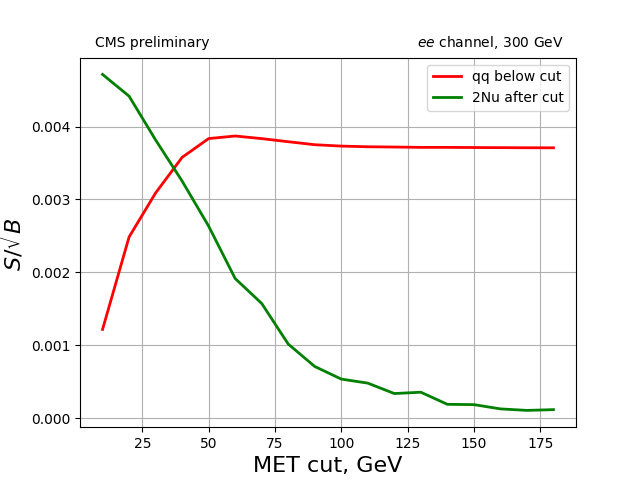
\includegraphics[width=0.45\textwidth]{ee_300_met.png}
    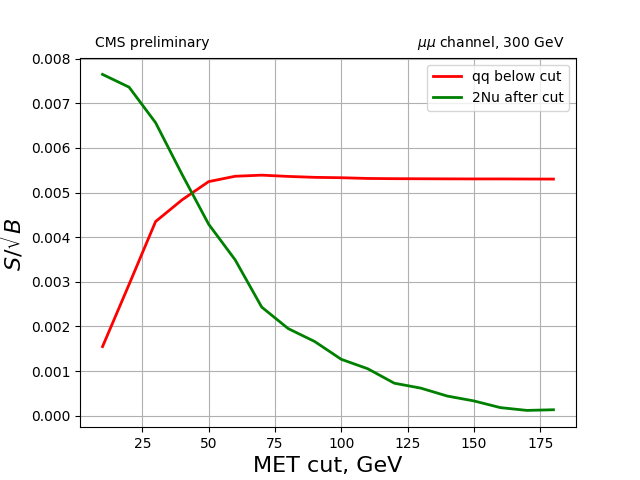
\includegraphics[width=0.45\textwidth]{mm_300_met.png}\\
    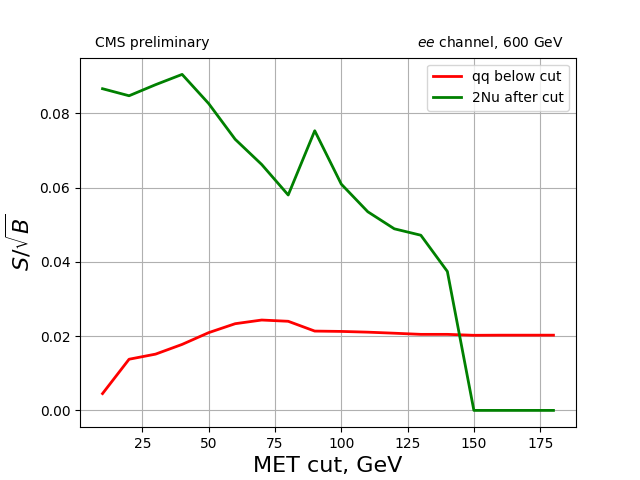
\includegraphics[width=0.45\textwidth]{ee_600_met.png}
    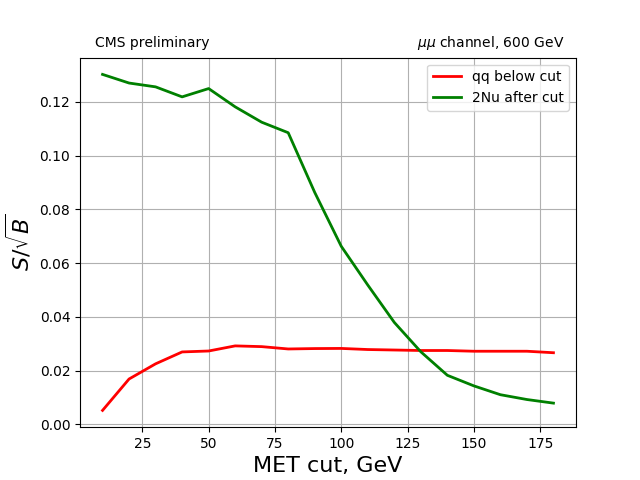
\includegraphics[width=0.45\textwidth]{mm_600_met.png}\\
    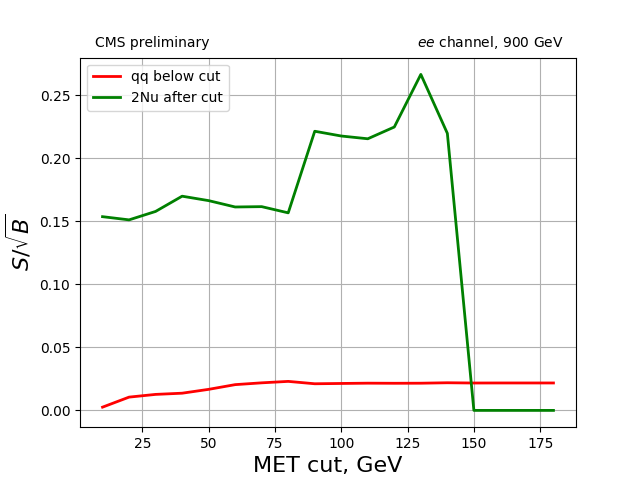
\includegraphics[width=0.45\textwidth]{ee_900_met.png}
    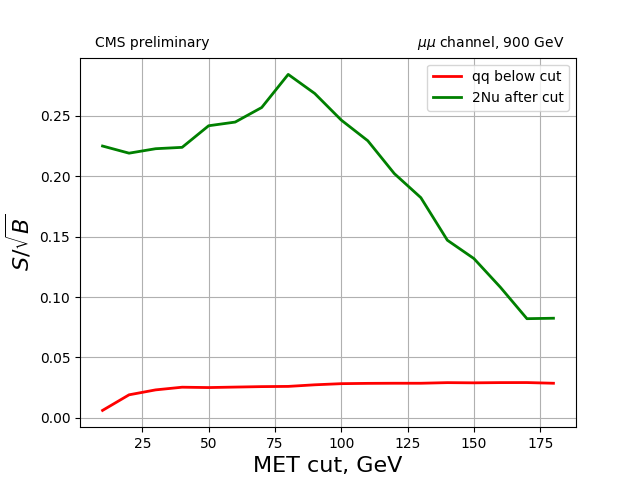
\includegraphics[width=0.45\textwidth]{mm_900_met.png}\\
    \caption[Optimisation of the MET selection for two $bbZZ$ analyses]{ Optimisation of the MET selection for two $bbZZ$ analyses. S and B stand for signal and background process' yields respectively. Significance-like figure of merit ($\sqrt{S}/B$) as a function of the MET cut is used to identify the best selection for each given mass hypothesis. Green curve shows the significance for this measurement, where events are kept above a given threshold. Red curve shows the  significance for the other $bbZZ$ measurement, where the MET requirement is inverted (events are kept below that threshold).  Top: 300 GeV mass. Middle: 600 GeV mass. Bottom: 900 GeV mass. On the left di-electron channel, di-muon channel is shown on the right. }
    \label{fig:met_cuts}
  \end{center}
\end{figure}

\begin{table}[H]
\begin{center}
\caption{The MET requirements as a function of the mass of the HH candidate. Selection values (the second column) are provided for different mass hypotheses (the first column) of the narrow resonance decaying to the HH system.}
\begin{tabular}{|c|c|} \hline
{Signal mass, GeV} &  \ETslash selection, GeV\\\hline
260-300     &                                \textgreater~40 \\
350-600     &                                \textgreater~75 \\
650-1000    &                                \textgreater~100 \\
\hline
\end{tabular}
\label{metCuts}
\end{center}
\end{table}

\subsection{Signal candidate construction and selection}

Two leptons of opposite sign and same flavor with the invariant mass higher than 76 GeV are selected as Z candidates. This mass requirement helps rejecting di-lepton candidates not corresponding to real Z bosons. Events with di-lepton mass higher than 76 GeV will be used for SR and $t\bar{t}$ CR. Additional Z mass selection will be discussed in the corresponding section later in this chapter. These on-shell Z bosons are assumed to come from the $H \to Z Z^*$ decays. The other Z boson, off-shell Z boson, decays to two neutrinos in our signature, and is represented by MET. Lorentz four-vectors of the di-lepton candidate and MET are added and the resulting four-vector represents the first Higgs boson candidate. 

The other Higgs boson is formed from the pair of b jets with the highest output value of the CMVA algorithm. No requirement is applied on existence or absence of other b jets in an event because such may be present due to a b jet misidentification or b jets resulting from pileup interactions or an underlying event. The invariant mass of the \HBB~candidate is required to be greater than 20 GeV to remove contamination from background events with low mass resonances that decay to two jets, such as events with J/psi, Upsilon or low energy QCD interactions. There is no upper requirement on the \HBB~ invariant mass. Together with the first Higgs boson, the constructed di-Higgs system approximates the double Higgs boson production that this measurement studies. 

The final double Higgs boson candidate (HH candidate) comprises the \Zll~candidate, the MET representing the \Znn~decay, and the \HBB~candidate. The four-momentum of this HH candidate is defined as the sum of the four momenta of the two leptons and two b jets in the candidate as well as the four momentum of the MET, defined in Sec. \ref{sec:cms_reco}.

HH system decays to a pair of b quarks and a pair of W bosons can also result in the same final state. The expected yields for the $bbWW$ channel with respect to the $bbZZ$ yields are comparatively small (1 to 4), because of the stringent kinematic selection on the di-lepton invariant mass. However, the contribution from the HH system decaying through the $bbWW$ intermediate state is still considered to be part of our signal in this measurement. The minimum requirement on the di-lepton mass is necessary to ensure that our measurement is orthogonal to the known HH search from CMS in the $bbVV$ channel that focused on $bbWW$ decays \cite{bbWW}, where only events with the di-lepton mass below 76 GeV were studied.

In collider physics, one of several common definitions of the transverse mass is given by:
$M_T=\sqrt( E^2- p_z^2)$. This quantity is widely used in the CMS searches for new particles. We proceed in the same fashion constructing our final variable - \mTHH, using the di-Higgs four-vector defined in the previous paragraphs. 

While up until this moment we had the same requirements for the search of the $radion/graviton \to HH$ for any heavy resonance mass, it is worth noting that at this point the analysis becomes mass point-specific. This is because the selection on the BDT discriminant (explained later) and the MET requirement differ with the mass hypothesis. When we compute limits for different radion or graviton hypotheses, we apply different selection criteria. 

Finally, the reader should be informed that if an event does not have enough physics objects suitable (as discussed in the objects selection section) for building the \Zll or \HBB candidates, or if the event does not pass candidate selection requirements on those objects or the full HH system, the event is discarded.

\subsection{Signal and control kinematic regions}

Three regions are defined: signal-enriched or signal region, and two CRs. The signal region is chosen such that the expected signal fraction is the largest there. Two control regions are defined such that they contain predominantly the background events with almost no signal. We define two CRS, one for each of the two main background sources: the CR for $t\bar{t}$ (CRTT) and the CR for Drell-Yan in association with jets (CRDY).

Two intermediate particles in the decay chain are nearly fully reconstructed, such as \HBB and \Zll. The signal region is defined in the phase space of \HBB and \Zll events. This corresponds to an area determined by the mass of the Higgs boson (125 GeV) and the mass of the Z boson ( 91.2 GeV). To account for the detector smearing effects, the mass windows near the pole masses are defined such that we select events within the \HBB mass range from 90 to 150 GeV and Z mass range from 76 to 106 GeV, see Fig. \ref{fig:regions}. In the CMS, these relatively standard  mass windows are chosen taking into account the detector resolution effects on a two b jet system and a di-lepton (and the natural width for a Z boson) mass and contain approximately 95$\%$ of true Higgs and Z boson candidates. The proportion of signal events is further increased with respect to background events by applying an additional requirement, the MVA requirement, which will be explained in the next section.

\begin{figure}[!htb]%hbpt?                                                                       
  \begin{center}
    %\raisebox{0.17\height}                                                                     
    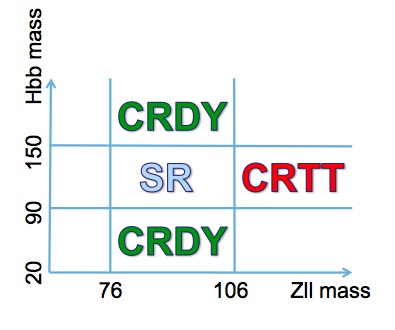
\includegraphics[width=0.45\textwidth]{regions.png}
    \caption[Analysis phase space with the signal and two control regions.]{ Signal region, control region \ttbar, and control region Drell-Yan in the phase space of \ZtoLL \ ~and ~\HBB ~masses.    }
    \label{fig:regions}
  \end{center}
\end{figure}

CRs are defined inverting the SR selection. Drell-Yan plus jets (or ``DY'' later for brevity) background process contains a real Z boson, while the two jets are random and have random invariant mass. We obtain the CRDY inverting the \HBB selection. For CRTT, $t\bar{t}$ events always have two b quarks whose invariant mass has a broad distribution, while they do not have a real Z boson. Thus, to select CRTT, we invert the \Zll selection and use only the events in the upper range of the Z mass, see Fig. \ref{fig:regions}. 

CRs are used to fit the event yield of the simulated background processes to the event yield in data and, thus, to determine the relative normalisations of $t\bar{t}$ and Drell-Yan background processes, which is done using CRTT and CRDY correspondingly. 

The efficiency of the candidate selection, up to this point, is summarised in the Table \ref{eff_upto_bdt}, where number are provided for the SR. The signal contributions are split into two components $bbZZ$ and $bbWW$, and are shown separately. The corresponding total numbers of events passing the selection are also given (the fourth column).

\begin{table}
\begin{center}
\caption{Number of events surviving the candidate selection and kinematic requirements. Numbers are given for $bbZZ$ and $bbWW$ contributions in the SR. Efficiency values are also provided (the third column) and are normalised to the initial event counts before any selection is applied. Di-muon channel is presented. Numbers for di-electron channel have the same trend but lower values since in the CMS, efficiencies for electrons are lower than for muons. }
\begin{tabular}{ |c|c|c|c| } \hline
{Process} & Mass, GeV & Efficiency, \% & Number of events \\\hline
bbWW & 300 &  0.2 & 85\\
bbZZ & 300 &  10.4 & 4511\\
bbWW & 900 &  0.1 & 23\\
bbZZ & 900 &  15.1 & 12963\\\hline
\end{tabular}
 \label{eff_upto_bdt}
\end{center}
\end{table}

\subsection{Signal region candidate selection with a multivariate technique}

After the SR and CRs have been defined, in the final step of the event selection we require the events in the SR to pass the threshold value of the BDT discriminant. An MVA discriminant that uses a boosted decision trees algorithm is trained considering a number of kinematic quantities of a candidate to be above a certain threshold. As this selection step is complex, it is described in a dedicated chapter: \ref{sec:BDT}.

\section{Multivariate selection in the signal region}

To reduce the background contamination in the SR, we employ a standard practice of CMS physics analyses of utilising the MVA discriminant. In this section, we will discuss which discriminating variables were used, how the MVA discriminant was constructed, and what are the efficiencies of the BDT selection for all major signal and background processes. 
\label{sec:BDT}

\subsection{Kinematic variables of a candidate}
\label{variables}

A  number of kinematic quantities can be constructed out of four-vectors that comprise candidates of our final state.  The distributions of these quantities in general differ for candidates originating from different background processes as opposed to for candidates from the hypothetical signal. 
           
In this section we discuss a set of kinematic quantities that are the most discriminating between the expected signal candidates and background candidates. This set of variables is used as an input for computing the multivariate discriminate that is later discussed in this section. In total, nine variables are chosen for this purpose and discussed here. About 30-40 other kinematic variables were considered at early stages of this data analysis. However, they were discarded as it was found that they do not improve the results of this measurement in a  significant way, while they increase considerably the complexity of the measurement.
           
Since the MVA selection requirement will be applied on a quantity computed based on these variables, the simulation has to  reproduce the main variables well. We will define each of the nine variables below. For SR and both CRs, we will show the comparison of distributions from data and simulation for each variable. Since the number of plots would be too large to show for two channels and two spin hypotheses, not to mention for all masses, we will include in this dissertation only di-muon channel plots for 300 GeV graviton mass hypothesis. However, all other relevant figures of the nine main variables, including the di-electron channel and other mass points,  were examined and discussed with CMS collaborators during the review of the measurement in CMS. They show a similar behaviour and agreement as those included here.
           
As we outlined before, even for simple physics objects the distributions from MC simulations and data have discrepancies. For more complex objects and candidates, these discrepancies become even larger. In general, MC simulations are not supposed to reproduce well very narrow regions of the kinematic phase space or align with the data perfectly at the high order in the QCD. Therefore, one normally adjusts the event yields (rates) of background processes using the normalisation values determined in the fit to data in the control regions. The distributions as they are, without the extra normalisations (from the fit) applied to the event yields of MC simulated background processes, are in general called pre-fit distributions. After the normalisations from the fit are applied on the rates of background processes, post-fit distributions are obtained. 

The list below summarises the set of variables used as input to the MVA discriminant:

\begin{itemize}

\item{\bfseries $\Delta R$ separation between two b jets.}
The $\Delta R$ (defined in the Section \ref{sec:cms}) separation between the b jets ($\Delta R_{b\ jets}$) gradually decreases as we start considering larger graviton or radion masses. This fact is explained by the Lorentz boost of the \HBB~system. When the heavy resonance produces two SM Higgs bosons, they are highly boosted. For the Higgs boson, which will further decay to a pair of b quarks (\HBB), the b quarks will come out of the decay almost collinear to each other with a minimal value of the $\Delta R_{b\ jets}$. For background processes this separation does not depends on the graviton or radion mass hypothesis. 

\item{\bfseries $\Delta R$ separation between two leptons.}
The distance between two leptons in the $\eta - \varphi$ space ($\Delta R_{leptons}$) tends to be smaller for the di-lepton system coming from the real Z bosons originated from the \HZZ~decays, in comparison to the $\Delta R_{leptons}$ distance between two random OSSF leptons produced by background processes. 

\item{\bfseries Missing transverse momentum.}
$\PTslash$ distribution coming from the off-shell Z bosons is constrained by the invariant mass of the parent Higgs boson and has, thus, a more narrow distribution. Contrary, the MET coming from $t\bar{t}$ background process can produce smaller and larger values of the MET. 

\item{\bfseries Invariant mass of the $\HBB$~candidate.} 
\HBB~mass for two b jets coming from real Higgs boson tends to be close to the SM Higgs boson invariant mass smeared by the b jet energy-momentum resolution, while the background candidates from unrelated b jets can have smaller and larger masses, especially if they come from the top quarks of the $t\bar{t}$ background.
           
\item{\bfseries Transverse momentum of the \HBB~candidate.} 
The transverse momentum of the \HBB~candidate ($p_T^{Hbb}$) tends to be have a relatively narrow peaky distribution for candidates coming from the hypothetical signal in comparison to broad distributions produced by the background processes. 

\item{\bfseries Invariant mass of the $ZZ^*$~system.} 
$ZZ^*$ mass of two Z bosons coming from the Higgs boson decay ($\HZZ$) tends to be close to the SM Higgs boson mass smeared by the \PTslash resolution, while the background candidates from DY production in association with jets can have random masses, which can be particularly large if they come from the DY production in association with several jets in addition to some instrumental MET present in the event.

\item{\bfseries Transverse momentum of the $ZZ^*$~system.} 
The transverse momentum of the \HZZ~candidate ($p_T^{Hzz}$) tends to be have a relatively narrow peaky distribution for candidates coming from the hypothetical signal in comparison to broad distributions produced by the background processes. 

\item{\bfseries Invariant mass of the Z boson candidate.} 
Z bosons coming from the Higgs boson have the invariant mass near the pole mass, while Z bosons from DY plus jets production can have a broader peak.

\item{\bfseries Transverse momentum of the Z boson candidate.} 
The transverse momentum of the Z candidate ($p_T^Z$) tends to be have a relatively narrow distribution for candidates coming from the real Z boson produced in the decays of the hypothetical signal in comparison to broad distributions of the $p_T^{\ell\ell}$, when di-lepton systems are produced by background processes. 

\end{itemize}
           
At this stage of the analysis description, we would like to refer the reader to the pre-fit plots (figures in the left columns). The figures are shown in the following order: all nine distributions in CRDY \ref{fig:MCcomparisons_mm_low_CRDY, fig:MCcomparisons_mm_low_CRDY_2}, in SR \ref{fig:MCcomparisons_mm_low_SR, fig:MCcomparisons_mm_low_SR}, and in CRTT \ref{fig:MCcomparisons_mm_low_CRTT, fig:MCcomparisons_mm_low_CRTT_2}. The simulated distributions are found in an acceptable agreement with those from the data and are judged to be adequate for a use in a multivariate discriminant construction discussed next. 

%~~~~~~~~~~~~~~~~~~~~~~~~~~~~~~~~~~~~~~~~~~~~~~~~~~~~~~~~~~~~~~~~~~~~~~~~~~~~~~~~~~~~~~~~~~~~~~~~~~~~                                                                            
\begin{figure}[H]
  \begin{center}
    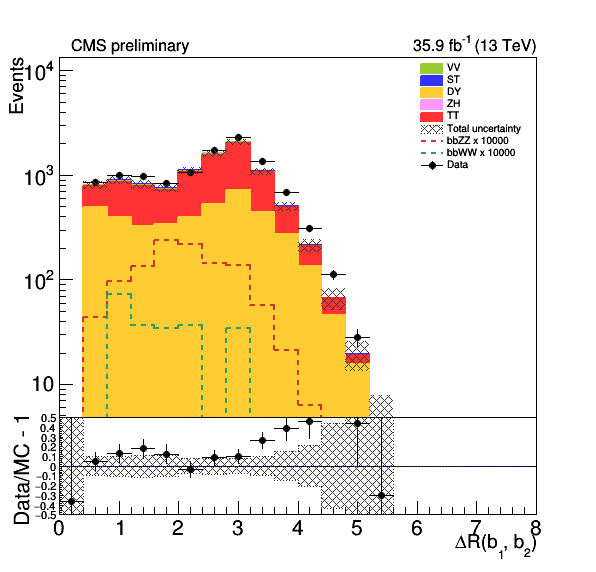
\includegraphics[width=0.31\textwidth]{figures/mm_300_april18/dR_bjets_mm_CRDY_prefit_plot_apr18.png}
    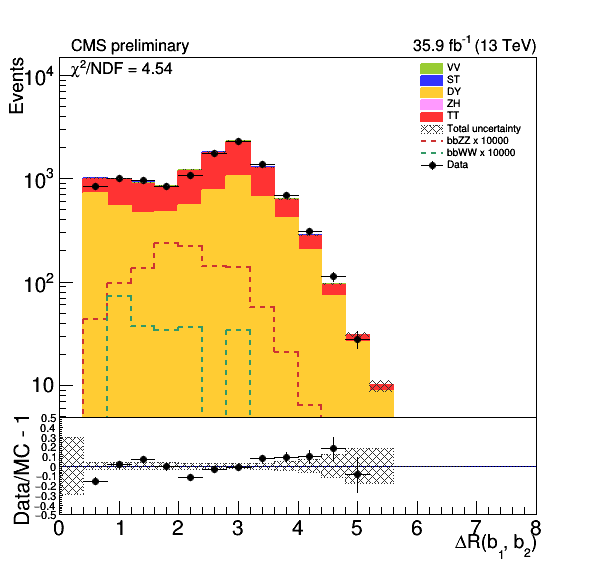
\includegraphics[width=0.31\textwidth]{figures/mm_300_april18/dR_bjets_mm_CRDY_FullPostfit_plot_apr18.png}\\
    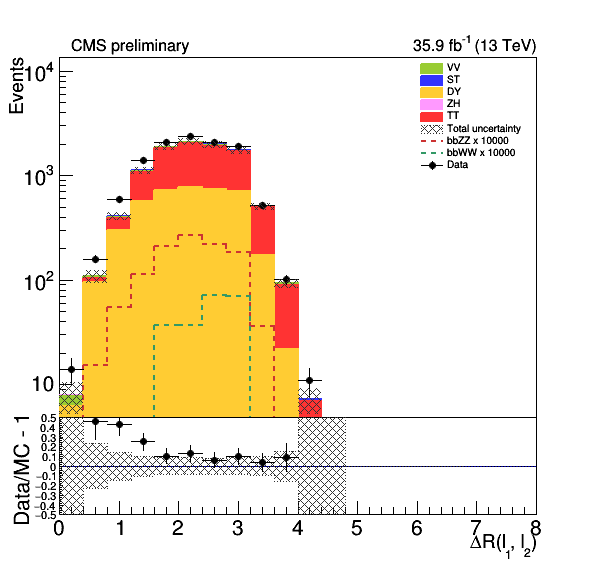
\includegraphics[width=0.31\textwidth]{figures/mm_300_april18/dR_leps_mm_CRDY_prefit_plot_apr18.png}
    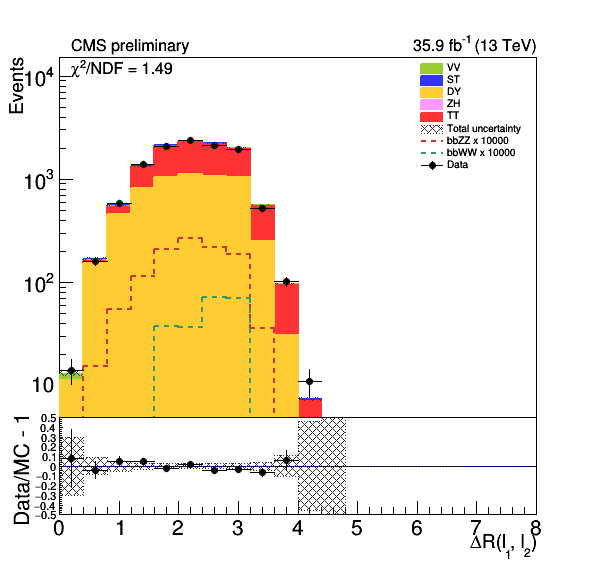
\includegraphics[width=0.31\textwidth]{figures/mm_300_april18/dR_leps_mm_CRDY_FullPostfit_plot_apr18.png}\\
%    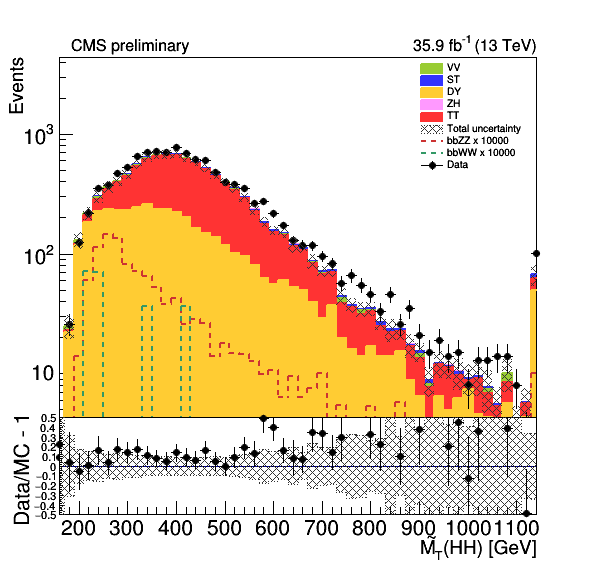
\includegraphics[width=0.31\textwidth]{figures/mm_300_april18/hhMt_mm_CRDY_prefit_plot_apr18.png}
   % 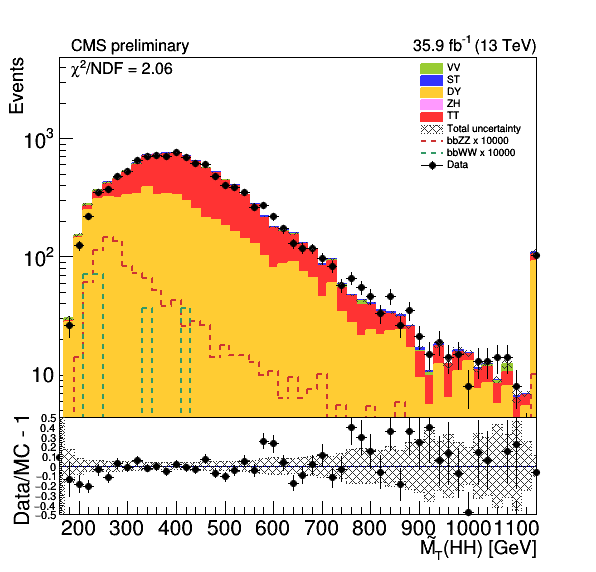
\includegraphics[width=0.31\textwidth]{figures/mm_300_april18/hhMt_mm_CRDY_FullPostfit_plot_apr18.png}\\
    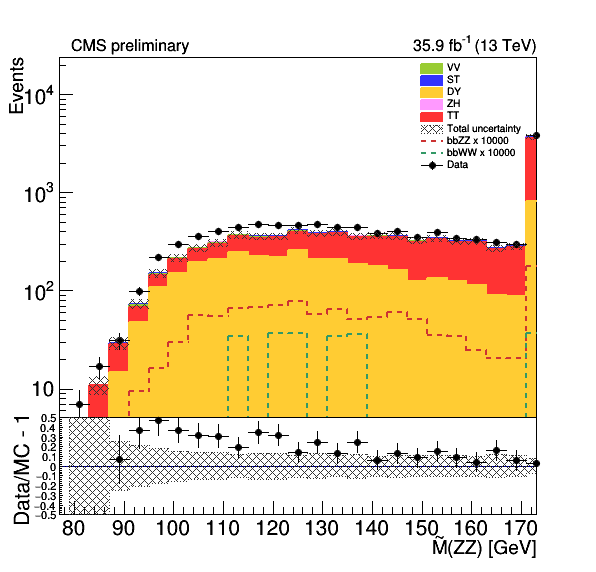
\includegraphics[width=0.31\textwidth]{figures/mm_300_april18/hmass0_mm_CRDY_prefit_plot_apr18.png}
    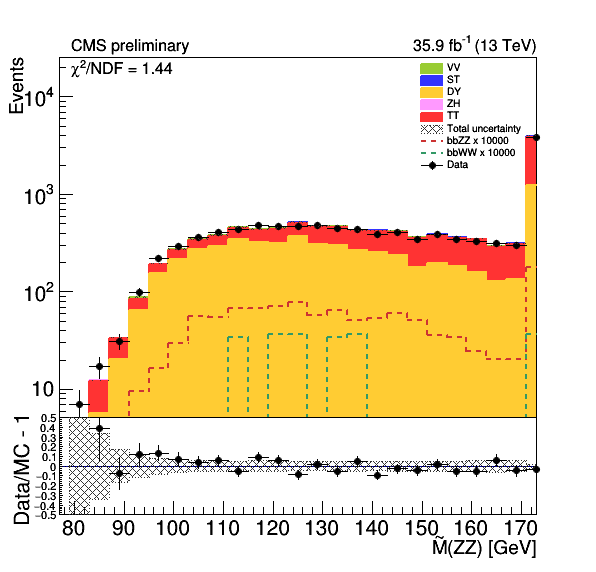
\includegraphics[width=0.31\textwidth]{figures/mm_300_april18/hmass0_mm_CRDY_FullPostfit_plot_apr18.png}\\
    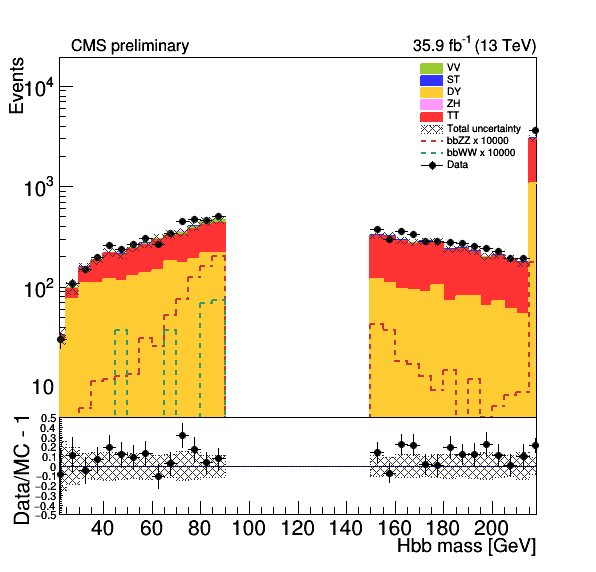
\includegraphics[width=0.31\textwidth]{figures/mm_300_april18/hmass1_mm_CRDY_prefit_plot_apr18.png}
    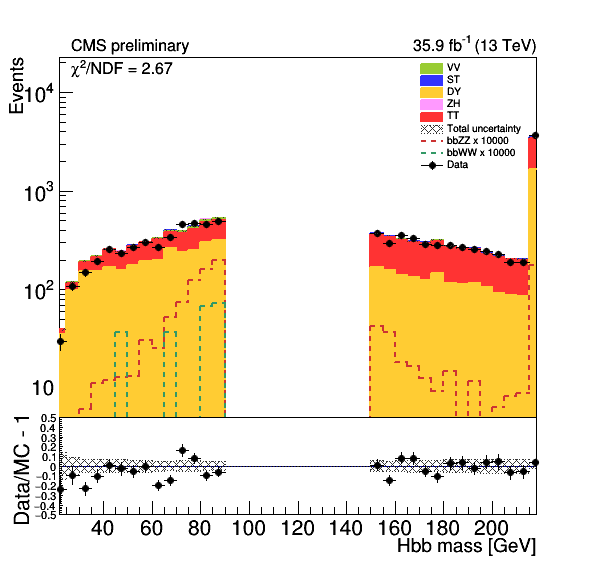
\includegraphics[width=0.31\textwidth]{figures/mm_300_april18/hmass1_mm_CRDY_FullPostfit_plot_apr18.png}\\
    \caption[Data-MC comparison in CRDY.]{Comparison of data and MC samples. 300 GeV, CRDY region, mm channel. Prefit plot on the left, Full Postfit plot on the right.}
    \label{fig:MCcomparisons_mm_low_CRDY}
  \end{center}
\end{figure}

\begin{figure}[H]
  \begin{center}
    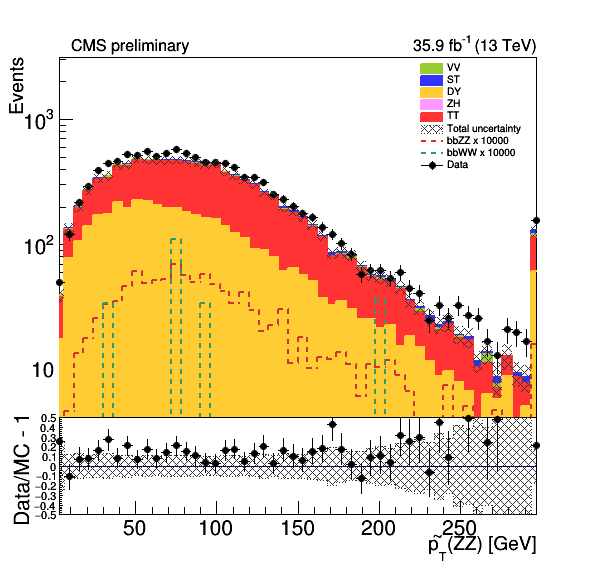
\includegraphics[width=0.31\textwidth]{figures/mm_300_april18/hpt0_mm_CRDY_prefit_plot_apr18.png}
    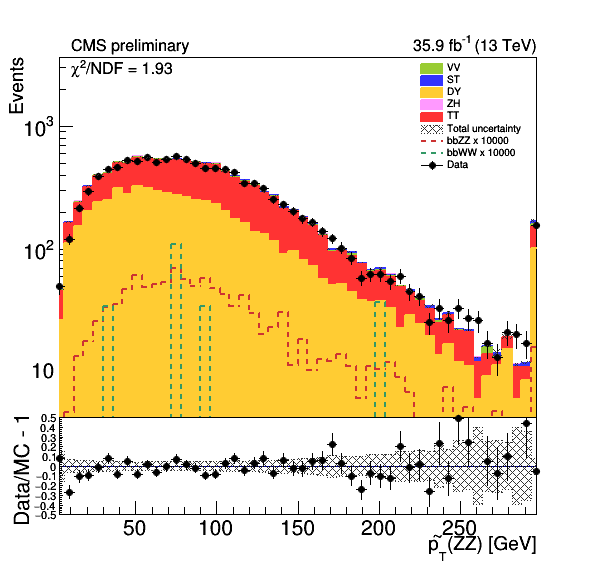
\includegraphics[width=0.31\textwidth]{figures/mm_300_april18/hpt0_mm_CRDY_FullPostfit_plot_apr18.png}\\
    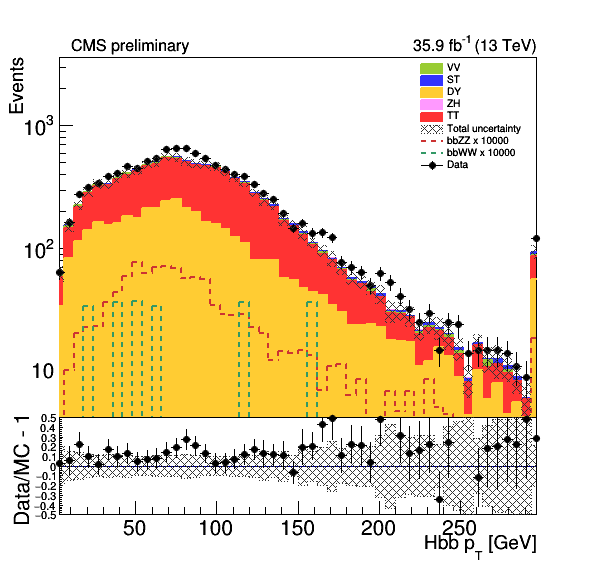
\includegraphics[width=0.31\textwidth]{figures/mm_300_april18/hpt1_mm_CRDY_prefit_plot_apr18.png}
    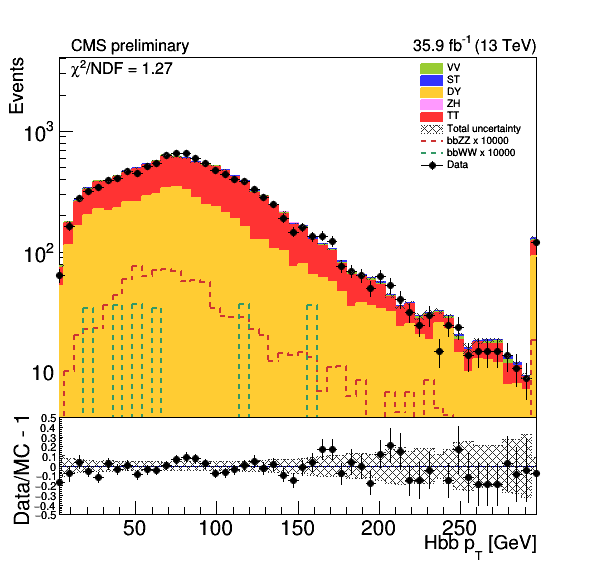
\includegraphics[width=0.31\textwidth]{figures/mm_300_april18/hpt1_mm_CRDY_FullPostfit_plot_apr18.png}\\
    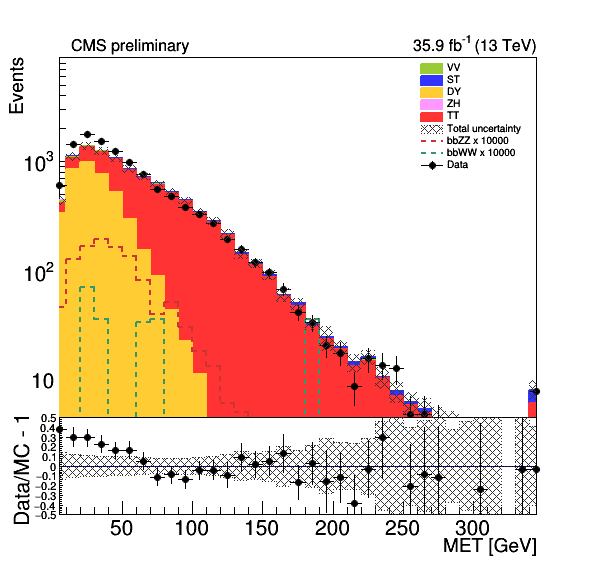
\includegraphics[width=0.31\textwidth]{figures/mm_300_april18/met_pt_mm_CRDY_prefit_plot_apr18.png}
    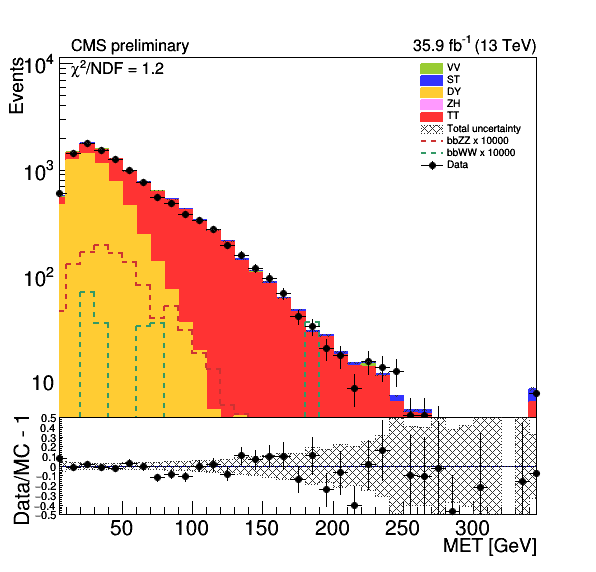
\includegraphics[width=0.31\textwidth]{figures/mm_300_april18/met_pt_mm_CRDY_FullPostfit_plot_apr18.png}\\
    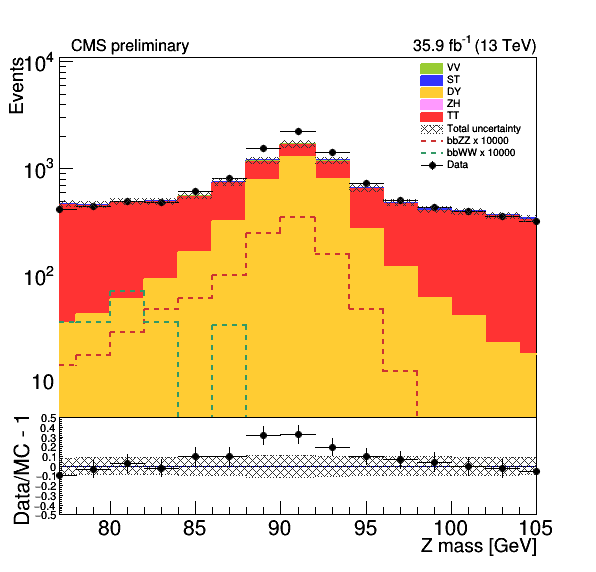
\includegraphics[width=0.31\textwidth]{figures/mm_300_april18/zmass_mm_CRDY_prefit_plot_apr21.png}
    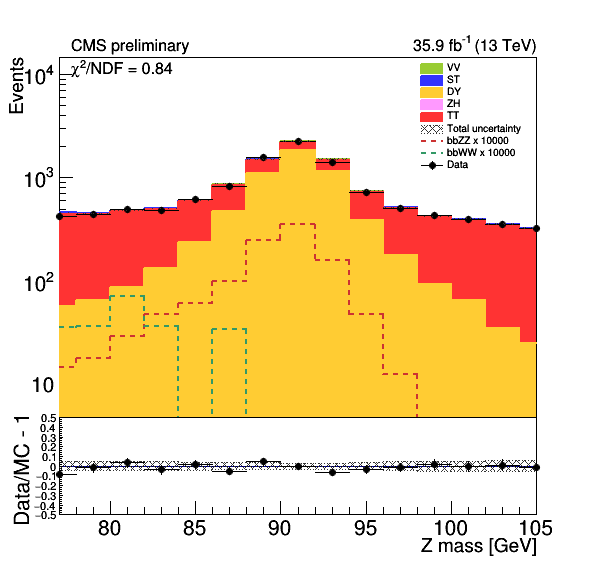
\includegraphics[width=0.31\textwidth]{figures/mm_300_april18/zmass_mm_CRDY_FullPostfit_plot_apr21.png}\\
%    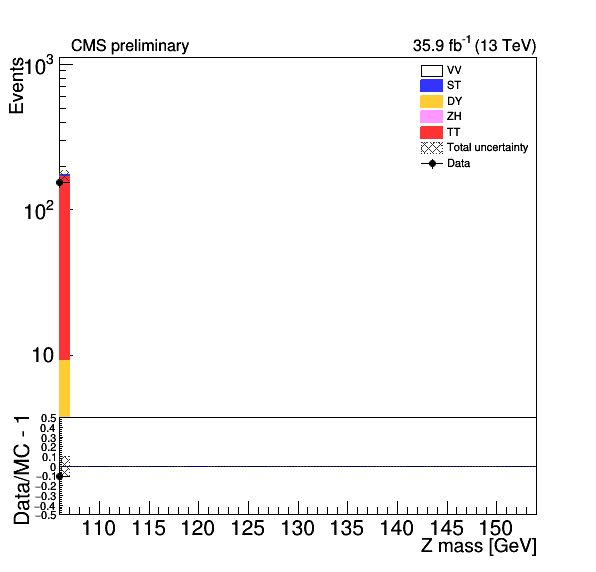
\includegraphics[width=0.31\textwidth]{figures/mm_300_april18/zmass_high_mm_CRDY_prefit_plot_apr18.png}                                                                      
%    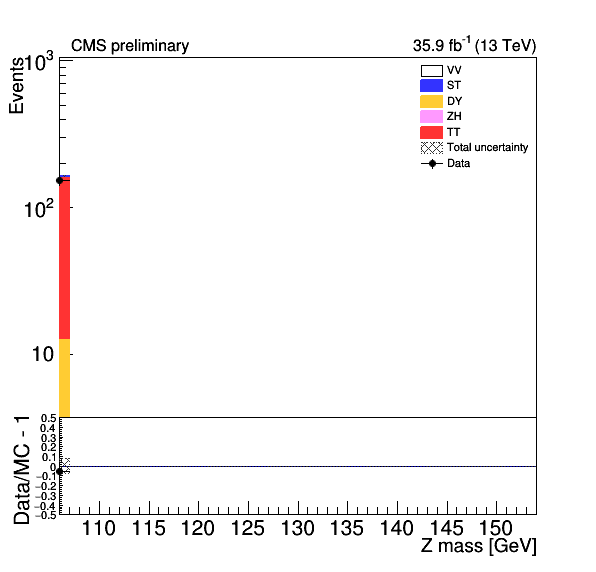
\includegraphics[width=0.31\textwidth]{figures/mm_300_april18/zmass_high_mm_CRDY_FullPostfit_plot_apr18.png}\\                                                               
    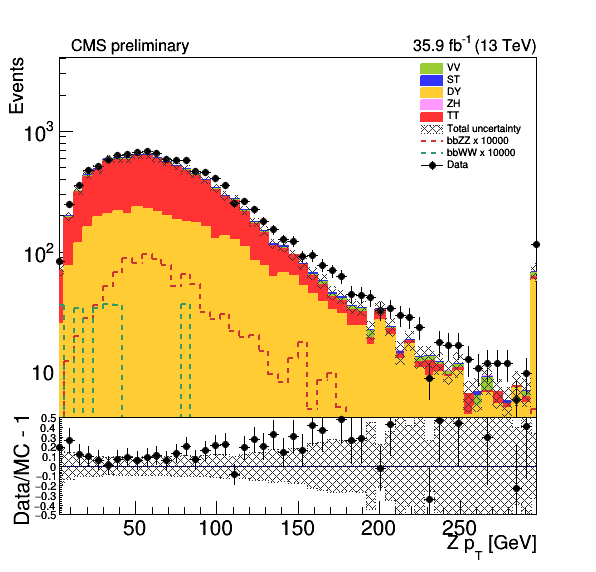
\includegraphics[width=0.31\textwidth]{figures/mm_300_april18/zpt0_mm_CRDY_prefit_plot_apr18.png}
    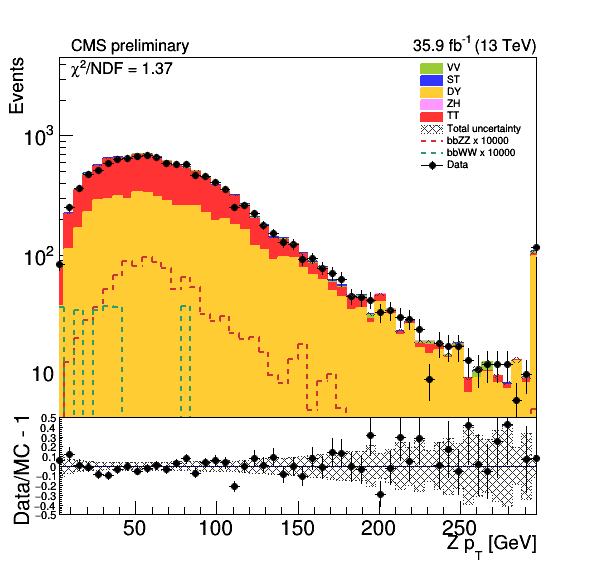
\includegraphics[width=0.31\textwidth]{figures/mm_300_april18/zpt0_mm_CRDY_FullPostfit_plot_apr18.png}\\
    \caption[Data-MC comparison in CRDY, other variables.]{Comparison of data and MC samples. 300 GeV, CRDY region, mm channel. Prefit plot on the left,           Full Postfit plot on the right.}
    \label{fig:MCcomparisons_mm_low_CRDY_2}
  \end{center}
\end{figure}

%~~~~~~~~~~~~~~~~~~~~~~~~~~~~~~~~~~~~~~~~~~~~~~~~~~~~~~~~~~~~~~~~~~~~~~~~~~~~~~~~~~~~~~~~~~~~~~~~~~~~                                                                                                                                                                                                                                                              
\begin{figure}[H]
  \begin{center}
    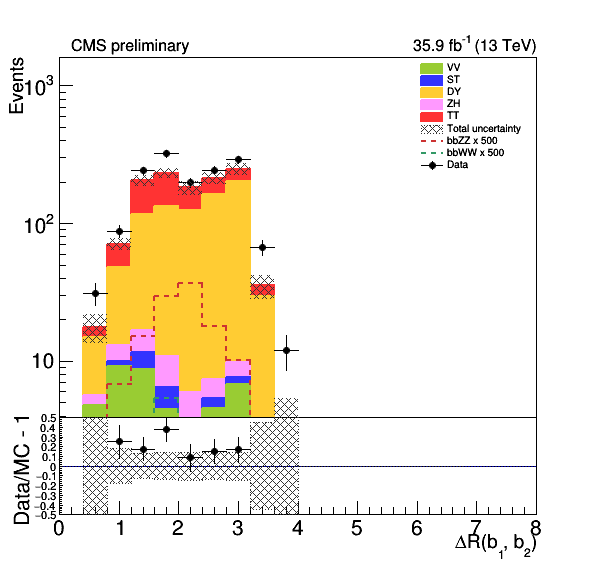
\includegraphics[width=0.31\textwidth]{figures/mm_300_SR_april21/dR_bjets_mm_SR_prefit_plot_apr21.png}
    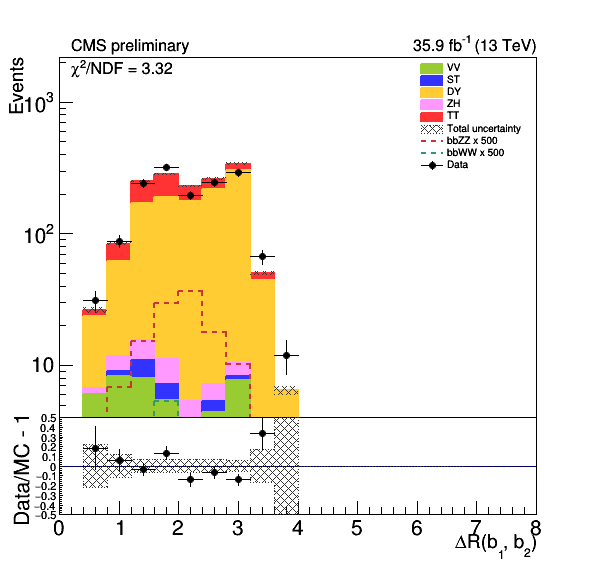
\includegraphics[width=0.31\textwidth]{figures/mm_300_SR_april21/dR_bjets_mm_SR_FullPostfit_plot_apr21.png}\\
    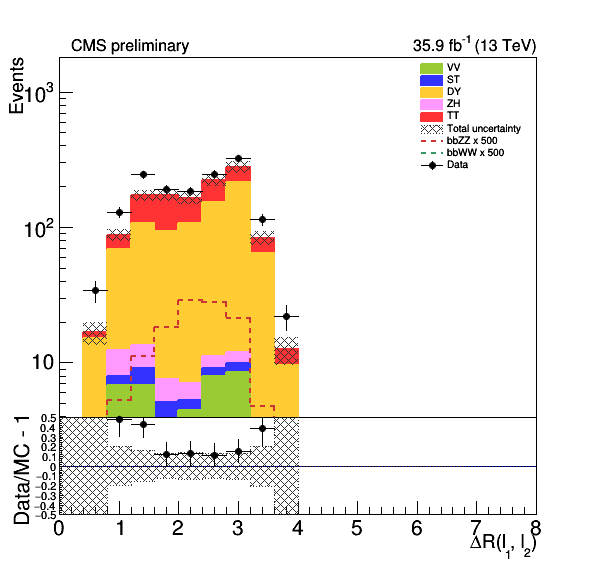
\includegraphics[width=0.31\textwidth]{figures/mm_300_SR_april21/dR_leps_mm_SR_prefit_plot_apr21.png}
    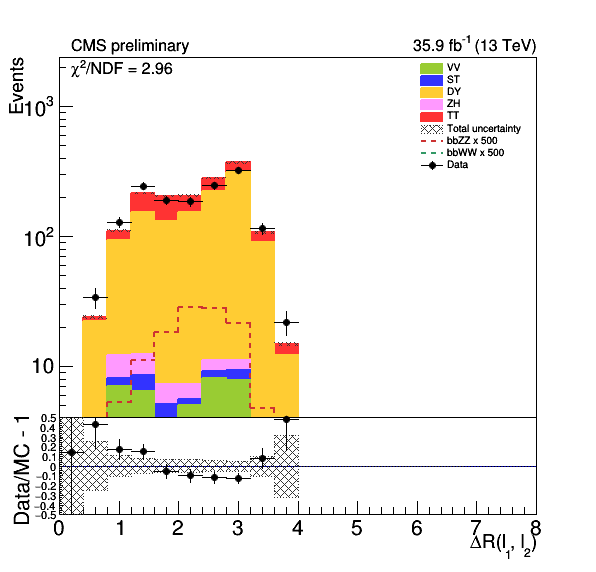
\includegraphics[width=0.31\textwidth]{figures/mm_300_SR_april21/dR_leps_mm_SR_FullPostfit_plot_apr21.png}\\
%    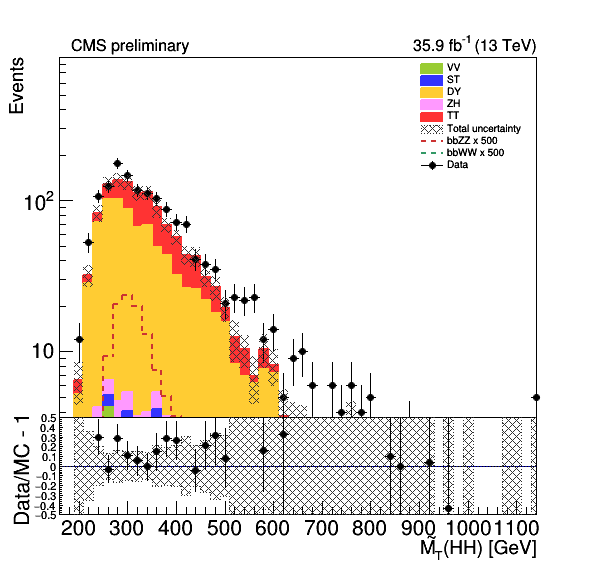
\includegraphics[width=0.31\textwidth]{figures/mm_300_SR_april21/hhMt_mm_SR_prefit_plot_apr21.png}
   % 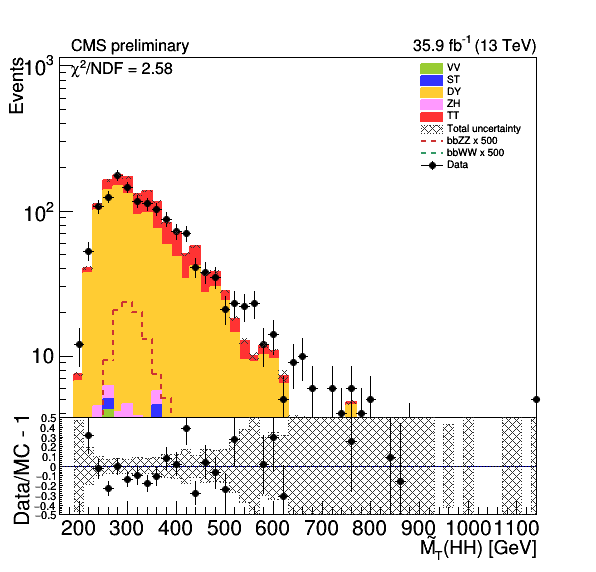
\includegraphics[width=0.31\textwidth]{figures/mm_300_SR_april21/hhMt_mm_SR_FullPostfit_plot_apr21.png}\\
    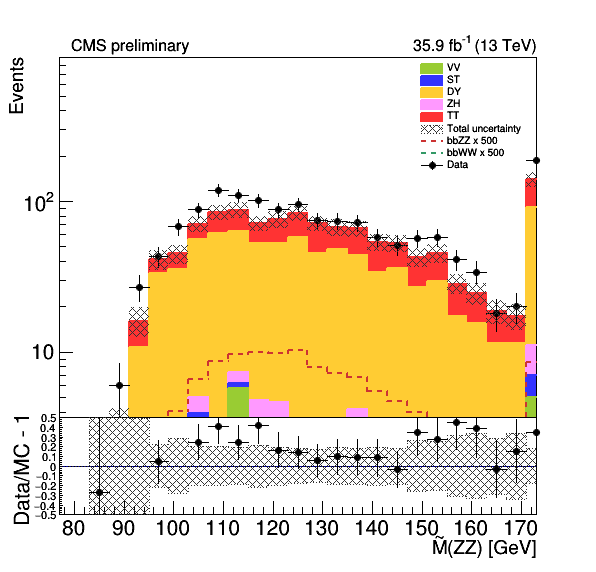
\includegraphics[width=0.31\textwidth]{figures/mm_300_SR_april21/hmass0_mm_SR_prefit_plot_apr21.png}
    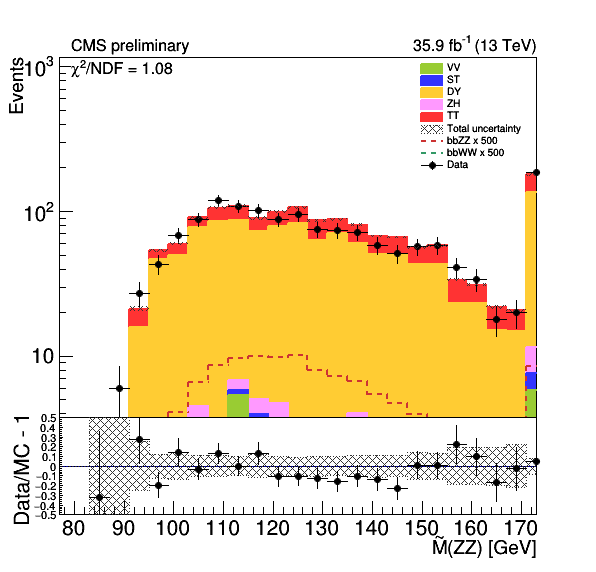
\includegraphics[width=0.31\textwidth]{figures/mm_300_SR_april21/hmass0_mm_SR_FullPostfit_plot_apr21.png}\\
    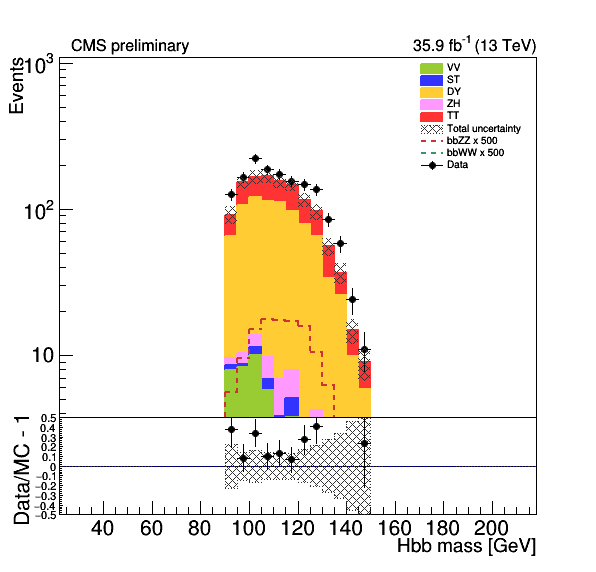
\includegraphics[width=0.31\textwidth]{figures/mm_300_SR_april21/hmass1_mm_SR_prefit_plot_apr21.png}
    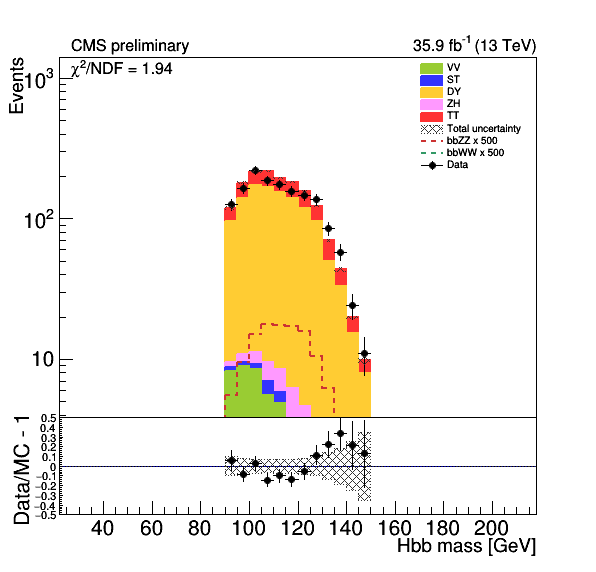
\includegraphics[width=0.31\textwidth]{figures/mm_300_SR_april21/hmass1_mm_SR_FullPostfit_plot_apr21.png}\\
    \caption[Data-MC comparison in SR.]{Comparison of data and MC samples. 300 GeV, SR region, mm channel. Prefit plot on the left,           Full Postfit plot on the right.}
    \label{fig:MCcomparisons_mm_low_SR}
  \end{center}
\end{figure}

\begin{figure}[H]
  \begin{center}
    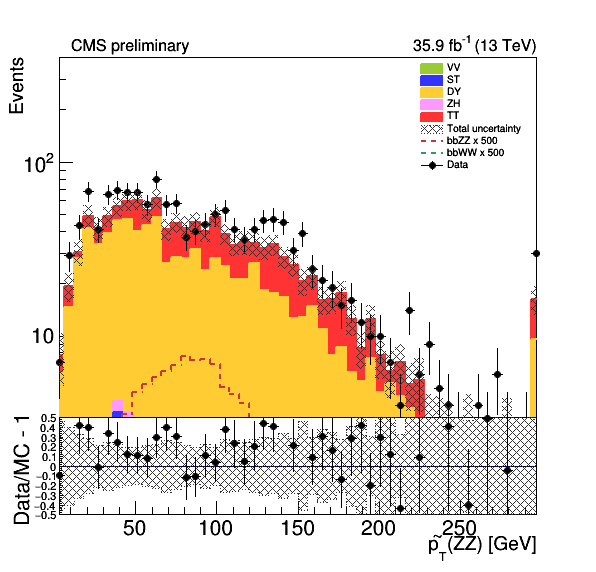
\includegraphics[width=0.31\textwidth]{figures/mm_300_SR_april21/hpt0_mm_SR_prefit_plot_apr21.png}
    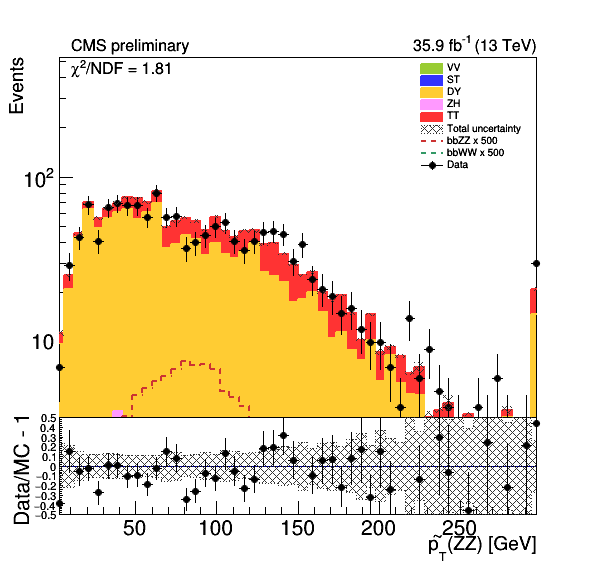
\includegraphics[width=0.31\textwidth]{figures/mm_300_SR_april21/hpt0_mm_SR_FullPostfit_plot_apr21.png}\\
    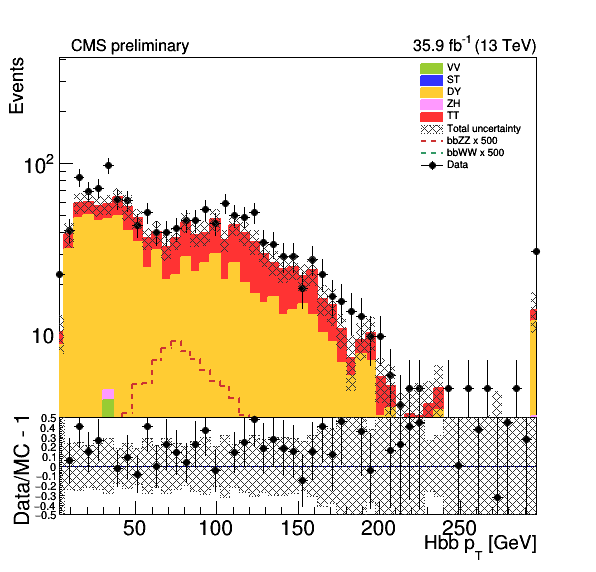
\includegraphics[width=0.31\textwidth]{figures/mm_300_SR_april21/hpt1_mm_SR_prefit_plot_apr21.png}
    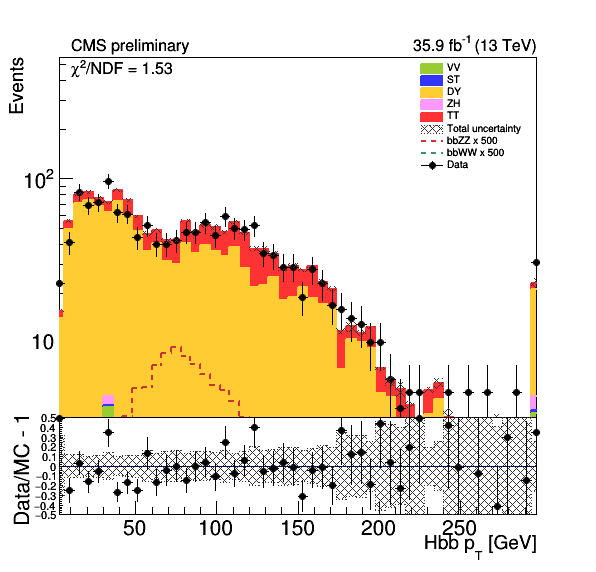
\includegraphics[width=0.31\textwidth]{figures/mm_300_SR_april21/hpt1_mm_SR_FullPostfit_plot_apr21.png}\\
    \includegraphics[width=0.31\textwidth]{figures/mm_300_SR_april21/met_pt_mm_SR_prefit_plot_apr21.png}
    \includegraphics[width=0.31\textwidth]{figures/mm_300_SR_april21/met_pt_mm_SR_FullPostfit_plot_apr21.png}\\
    \includegraphics[width=0.31\textwidth]{figures/mm_300_SR_april21/zmass_mm_SR_prefit_plot_apr21.png}
    \includegraphics[width=0.31\textwidth]{figures/mm_300_SR_april21/zmass_mm_SR_FullPostfit_plot_apr21.png}\\
    \includegraphics[width=0.31\textwidth]{figures/mm_300_SR_april21/zpt0_mm_SR_prefit_plot_apr21.png}
    \includegraphics[width=0.31\textwidth]{figures/mm_300_SR_april21/zpt0_mm_SR_FullPostfit_plot_apr21.png}\\
    \caption[Data-MC comparison in SR, other variables.]{Comparison of data and MC samples. 300 GeV, SR region, mm channel. Prefit plot on the left,           Full Postfit plot on the right.}
    \label{fig:MCcomparisons_mm_low_SR_2}
  \end{center}
\end{figure}

%~~~~~~~~~~~~~~~~~~~~~~~~~~~~~~~~~~~~~~~~~~~~~~~~~~~~~~~~~~~~~~~~~~~~~~~~~~~~~~~~~~~~~~~~~~~~~~~~~~~~                                                                            
\begin{figure}[H]
  \begin{center}
    \includegraphics[width=0.31\textwidth]{figures/mm_300_april18/dR_bjets_mm_CRTT_prefit_plot_apr18.png}
    \includegraphics[width=0.31\textwidth]{figures/mm_300_april18/dR_bjets_mm_CRTT_FullPostfit_plot_apr18.png}\\
    \includegraphics[width=0.31\textwidth]{figures/mm_300_april18/dR_leps_mm_CRTT_prefit_plot_apr18.png}
    \includegraphics[width=0.31\textwidth]{figures/mm_300_april18/dR_leps_mm_CRTT_FullPostfit_plot_apr18.png}\\
 %   \includegraphics[width=0.31\textwidth]{figures/mm_300_april18/hhMt_mm_CRTT_prefit_plot_apr18.png}
    %\includegraphics[width=0.31\textwidth]{figures/mm_300_april18/hhMt_mm_CRTT_FullPostfit_plot_apr18.png}\\
    \includegraphics[width=0.31\textwidth]{figures/mm_300_april18/hmass0_mm_CRTT_prefit_plot_apr18.png}
    \includegraphics[width=0.31\textwidth]{figures/mm_300_april18/hmass0_mm_CRTT_FullPostfit_plot_apr18.png}\\
    \includegraphics[width=0.31\textwidth]{figures/mm_300_april18/hmass1_mm_CRTT_prefit_plot_apr18.png}
    \includegraphics[width=0.31\textwidth]{figures/mm_300_april18/hmass1_mm_CRTT_FullPostfit_plot_apr18.png}\\
    \caption[Data-MC comparison in CRTT]{Comparison of data and MC samples. 300 GeV, CRTT region, mm channel. Prefit plot on the left,           Full Postfit plot on the right.}
    \label{fig:MCcomparisons_mm_low_CRTT}
  \end{center}
\end{figure}

\begin{figure}[H]
  \begin{center}
    \includegraphics[width=0.31\textwidth]{figures/mm_300_april18/hpt0_mm_CRTT_prefit_plot_apr18.png}
    \includegraphics[width=0.31\textwidth]{figures/mm_300_april18/hpt0_mm_CRTT_FullPostfit_plot_apr18.png}\\
    \includegraphics[width=0.31\textwidth]{figures/mm_300_april18/hpt1_mm_CRTT_prefit_plot_apr18.png}
    \includegraphics[width=0.31\textwidth]{figures/mm_300_april18/hpt1_mm_CRTT_FullPostfit_plot_apr18.png}\\
    \includegraphics[width=0.31\textwidth]{figures/mm_300_april18/met_pt_mm_CRTT_prefit_plot_apr18.png}
    \includegraphics[width=0.31\textwidth]{figures/mm_300_april18/met_pt_mm_CRTT_FullPostfit_plot_apr18.png}\\
    \includegraphics[width=0.31\textwidth]{figures/mm_300_april18/zmass_high_mm_CRTT_prefit_plot_apr18.png}
    \includegraphics[width=0.31\textwidth]{figures/mm_300_april18/zmass_high_mm_CRTT_FullPostfit_plot_apr18.png}\\
    \includegraphics[width=0.31\textwidth]{figures/mm_300_april18/zpt0_mm_CRTT_prefit_plot_apr18.png}
    \includegraphics[width=0.31\textwidth]{figures/mm_300_april18/zpt0_mm_CRTT_FullPostfit_plot_apr18.png}\\
    \caption[Data-MC comparison in CRTT, other variables.]{Comparison of data and MC samples. 300 GeV, CRTT region, mm channel. Prefit plot on the left,           Full Postfit plot on the right.}
    \label{fig:MCcomparisons_mm_low_CRTT_2}
  \end{center}
\end{figure}

\subsection{Multivariate discriminant: a BDT classifier}

In HEP in many areas, such as an object identification, a reduction of the background contribution in the signal region, etc., there are needs to discriminate a ``signal'' from one or several ``backgrounds''. The discriminating algorithms can use a single physical variable for signal-background separation, or several variables. The way an algorithm uses the input variables can be of a sequential nature, or through some non-linear dependence. The Higgs boson discovery, in part, was possible due to an employed BDT approach, where several variables are combined into an artificial BDT score or output. The BDT output, as a higher-level construct, has no direct physical interpretation. However, due to the shown gain in signal-background separation performance, the BDT has been successfully used for years for the final classification decision. 

Multivariate discriminants (or models or classifiers) based on the BDT or other algorithms are constructed using machine learning (ML) techniques. Now, almost at every stage of the HEP data analysis, starting from the track reconstruction, through the object identification and the signal region purification, up to the construction of the final discriminating MVA variable, physicists rely on the ML methods.
           
In simple terms, the ML procedure consists of the training and testing stages (sometimes also the validation stage is added). First, the data is split into two non-overlapping sets: a train and a test data. Then, the classifier is trained, when the model is learning the patterns in the train data. After that, the performance of the model is tested using the independent test data. 

After the training procedure, ML algorithm produce a discriminator, which is a function that is related to the likelihood of an event to belong to a signal or to a background category. Here and in other parts of the thesis, we are describing the BDT procedure, which is a non-parametric supervised learning method used for classification; other MVA methods that are not related to this measurement, are well-explained in \cite{book:411471}. 

Every analysts would always like to have a classifier that has a low bias and a low variance. A bias is a difference between the average prediction of our model and the correct value, which we are trying to predict. A classifier with a high bias oversimplifies the model and does not take into account all the nuances of a given train data. Therefore, one prefers a low bias models, which are flexible and perform well both on the train and test data, and always provide a stable good separation between the signal and background hypotheses. A variance is the variability of model prediction for a given data point. A variance is related to the spread of our data. A model with high variance learns almost every single pattern in the train data and, therefore, will not generalise well, when given new unseen data. As a result, models with a high variance achieve the best scores using the train data but perform poorly on the test data. Thus, one prefers a low variance models, which are robust when applying the trained classifiers on a dataset that is statistically independent from the one used for training.

One of the most popular ML algorithms in HEP is based on the boosted decision trees (BDT). A single decision tree is a sequence of simple binary splits on each of the input variables. The tree, thus, can be depicted as a multidimensional set of selections on input space. The tree assigns a score of +1 or -1 if a given event is signal or background-like. The key elements in each step of the BDT spilts are the variables used for the selection and the positions of the selections. Both are determined using an impurity criterion $I(p_n)$, which is a function of the signal purity $p_n$ in tree node $n$. The signal purity is defined as a ratio of the signal contribution to the total number of signal and background events, $p_n = S/(S+B)$. The impurity criterion is chosen such that it is at the minumum when $p_n$=0 or $p_n$=1. These values would give a perfect signal-background discrimination. The criterion is at the maximum, when $p_n$=0.5, which means no discrimination is achieved. 
Each split maximises the gain function $G=I(p_n) - f_1I(p_{c1})-f_2I(p_{c2})$. In this formulation of $G$, the labels c1 and c2 refer to chid nodes of the parent node, and $f1$ and $f2$ are the fractions of events of the parent node that are found in child nodes c1 and c2, respectively. As a definition of the impurity criterion for this measurement, the Gini coefficient is used: $I_G(p_n) = ??2 p_n \cdot (1?p_n)$. 

The tree keeps applying the selection on the input variables until either a maximum depth is reached (a number of consecutive splits), or a minimum number of events in the final child nodes are attained. The problem with such a tree growing procedure is that it is prone to overtraining, which means the model will not generalise well and have a high variance. One way to deal with BDT overtraining is boosting. 
The idea behind boosting is, that signal events
 from the training sample that end up in a background node or vice versa, are given intentionally large weights (a penalty). These weights are normally significantly larger than the weights for events with
 the correct leave node prediction. Such penalty procedure reweighs the train data and then new decision trees are created. The boosting is applied hundreds of times, which produces a set of new reweighed trees (a forest). Intuitively, the boosting is a method in which a large number of shallow trees, which have only a few splits, are combined by taking a weighted average of their output scores. The discriminating power of a single shallow tree is usually poor, but such a tree is less prone to overtraining, therefore, when combined, the ensemble of these trees produces a model with a high and stable performance.
 
For the boosting algorithm, we chose the gradient boosting method, as is implemented in the popular MVA package for HEP - TMVA \cite{Hocker:2007ht}.  Gradient boosting can be thought of as a function expansion approach. In this case each tree corresponds to a summand. The parameters for each summand (tree) are determined by minimising of an error function. In the TMVA implementation, the binomial log-likelihood loss function is used. The adopted procedure follows the greedy algorithm approach - only one tree is modified at a time, while the other trees remain invariable.

 Several decision trees of the BDT procedure, that is employed in the analysis, are shown below. This training was done in the d-electron channel. In all figures produced by the TMVA, the index 0 refers to \HZZ~candidate and index 1 refers to \HBB~candidate. For example, ``hmass1'' denotes the mass of the \HZZ~candidate, ``hpt0'' denotes the $p_T$ of the \HBB~candidate, etc. For the Z boson candidate, the on-shell Z boson decaying to charged leptons, \Zll, has either an index 0 or the index is dropped. The closer the node color is to blue, the more the event is classified as signal-like, same idea is illustrated with the red color for background events. \label{TMVA_notation}

Di-electron and di-muon channels have been trained separately and the BDT metrics (discussed later in this chapter) show similar performance. That is why to save the space, in this chapter we show mostly figures related to the di-electron channel.
           
 \begin{figure}[H]
  \begin{center}
    \includegraphics[width=0.94\textwidth]{BDT_0.pdf}
    \includegraphics[width=0.94\textwidth]{BDT_1.pdf}\\
     \caption[BDT trees 1 and 2.]{BDT trees 1 and 2 (indexing starts from 0). These trees relied on: the mass and the $p_T$ of the \Zll~candidate, $\Delta R$ separation between two b jets,  the mass of the \HBB~candidate, and the $p_T$ of the $ZZ^*$ system. The TMVA notation is explained in \ref{TMVA_notation}.}
    \label{fig:bdt_trees}
  \end{center}
\end{figure}

\begin{figure}[H]
  \begin{center}
    \includegraphics[width=0.94\textwidth]{BDT_399.pdf}
    \includegraphics[width=0.94\textwidth]{BDT_400.pdf}\\
     \caption[BDT trees 400 and 401.]{BDT trees 400 and 401 (indexing starts from 0). These trees relied on: the $p_T$ of the \Zll~candidate, 
     $\Delta R$ separation between two b jets,
     $\Delta R$ separation between two charged leptons, 
      the $p_T$ of the \HBB~candidate, and the mass and the $p_T$ of the $ZZ^*$ system. The TMVA notation is explained in \ref{TMVA_notation}.}    
      \label{fig:bdt_trees_2}
  \end{center}
\end{figure}

\begin{figure}[H]
  \begin{center}
    \includegraphics[width=0.94\textwidth]{BDT_798.pdf}
    \includegraphics[width=0.94\textwidth]{BDT_799.pdf}\\
     \caption[BDT trees 799 and 800.]{BDT trees 799 and 800 (indexing starts from 0). These trees relied on: the $p_T$ of the \Zll~candidate, 
     $\Delta R$ separation between two b jets,
     $\Delta R$ separation between two charged leptons, 
      the mass of the \HBB~candidate, and the mass of the $ZZ^*$ system. The TMVA notation is explained in \ref{TMVA_notation}.}       
     \label{fig:bdt_trees_3}
  \end{center}
\end{figure}
           
The BDT discriminant (later the BDT for brevity) is trained on a pure sample of signal and background events from simulation, using the train data. The  properties of the discriminant are studied on an independent testing sample of pure signal and background events, using the test data. The Deep Neural Network (DL) approach also has been studies, however, due to the lack of the event statistics, the DL approach could not offer a performance higher than the one achieved with the BDT, and thus, was abandoned. Training 16 BDTs per the spin hypothesis seems unpractical since our data analysis is dominated by the statistical errors. Instead, we follow an approach of other HH analyses \cite{HH_combination}: we split the range from 250 to 1000 into two regions: low mass (250 to 450 GeV) and high mass (500 to 1000 GeV) regions. This separation boundary at 450 GeV was optimised first using ROC curves (described later in this section), then running the whole analysis chain all the way to the final limits. This procedure not only saves CPU cycles, training two BDTs instead of sixteen, but mostly increases the statistics and improves the robustness of the trained BDT. 
           
During the training procedure, some variables provide more discriminating power and on average are used more often than others. The more often the variable is used, the higher is its importance. The tables below show the ranking and average importance of each of the BDT training: low and high mass regions, di-electron and di-muon channels, see Tables \ref{tab:importance_ee_low, tab:importance_mm_high, tab:importance_mm_low, importance_mm_high}. 

\noindent\begin{table}[H]
   \centering
   \begin{tabular}{|c| l |c|}\hline
     Rank & Variable & Importance, \% \\\hline
     1 & $\Delta R_{b\ jets}$ & 13.9 \\ 
     2 & MET & 12.1 \\ 
     3 & Mass of $\HBB$~candidate & 11.9 \\ 
     4 & $p_T^{ZZ^*}$ & 11 \\ 
     5 & $\Delta R_{leptons}$ & 10.9 \\ 
     6 & $p_T$ of $\HBB$~candidate & 10.7 \\ 
     7 & $p_T$ of Z boson candidate & 10.2 \\ 
     8 & Mass of $ZZ^*$ system & 10.1 \\ 
     9 & Mass of Z boson candidate & 9.26 \\ 
     \hline
   \end{tabular}
   \captionof{table}{Di-electron channel. Relative importance of the input variables in the low mass BDT training.}
   \label{tab:importance_ee_low}
\end{table}
\begin{table}
   \centering
   \begin{tabular}{|c| l |c|}\hline
     Rank & Variable & Importance, \% \\\hline
     1 & $\Delta R_{leptons}$ & 14.1 \\ 
     2 & Mass of $\HBB$~candidate & 13.7 \\ 
     3 & $\Delta R_{b\ jets}$ & 13.2 \\ 
     4 & $p_T$ of $\HBB$~candidate & 12.1 \\ 
     5 & $p_T$ of Z boson candidate & 11.5 \\ 
     6 & $p_T^{ZZ^*}$ & 11.3 \\ 
     7 & MET & 10.3 \\ 
     8 & Mass of $ZZ^*$ system & 7.7 \\ 
     9 & Mass of Z boson candidate & 6.1 \\ 
     \hline
   \end{tabular}
   \captionof{table}{Di-electron channel. Relative importance of the input variables in the high mass BDT training.}
   \label{tab:importance_ee_high}
\end{table}

\vspace{2cm}
%%%%%%%%%%%%%%%%%%%%%%%%
%%%%%%%%%%%%%%%%%%%%%%%%
\noindent\begin{table}[H]
   \centering
   \begin{tabular}{|c| l |c|}\hline
     Rank & Variable & Importance, \% \\\hline
     1 & $\Delta R_{b\ jets}$ & 13 \\ 
     2 & MET & 12.2 \\ 
     3 & Mass of $\HBB$~candidate & 11.9 \\ 
     4 & $p_T$ of $\HBB$~candidate & 11.3 \\ 
     5 & $p_T$ of Z boson candidate & 11.1 \\ 
     6 & $p_T^{ZZ^*}$ & 10.9 \\ 
     7 & $\Delta R_{leptons}$ & 10.5 \\ 
     8 & Mass of $ZZ^*$ system & 9.7 \\ 
     9 & Mass of Z boson candidate & 9.5 \\ 
     \hline
   \end{tabular}
   \captionof{table}{Di-muon channel. Relative importance of the input variables in the low mass BDT training.}
   \label{tab:importance_mm_low}
\end{table}
\begin{table}
   \centering
   \begin{tabular}{|c| l |c|}\hline
     Rank & Variable & Importance, \% \\\hline
     1 & Mass of $\HBB$~candidate & 13.8 \\ 
     2 & $\Delta R_{b\ jets}$ & 13.1 \\ 
     3 & $\Delta R_{leptons}$ & 12.9 \\ 
     4 & $p_T$ of \HBB~candidate & 11.7 \\ 
     5 & $p_T^{ZZ^*}$ & 11.3 \\ 
     6 & $p_T$ of Z boson candidate & 11.1 \\ 
     7 & MET & 11 \\ 
     8 & Mass of $ZZ^*$ system & 8.8 \\ 
     9 & Mass of Z boson candidate & 6.2 \\ 
     \hline
   \end{tabular}
   \captionof{table}{Di-muon channel. Relative importance of the input variables in the high mass BDT training.}
   \label{tab:importance_mm_high}
\end{table}

The correlations among the input variables are shown in the Figs. ~\ref{fig:ele_cors_low}, ~\ref{fig:ele_cors_high}, ~\ref{fig:muon_cors_low}, ~\ref{fig:muon_cors_high}. For low mass training, signal samples for mass hypotheses from 250 to 450 GeV are combined together and represent the ``signal''. Similarly is done for high mass training - it is a mix of signal samples for mass hypotheses from 500 to 1000 GeV. For background samples, the ``background'' is a mix of samples of two main background processes: DY in association with jets and $t\bar{t}$ production, weighted by the cross section value.

\begin{figure}[tbp]
  \begin{center}
   \includegraphics[width=0.75\textwidth]{bdtPlots_eles/low_corS.pdf}
   \includegraphics[width=0.75\textwidth]{bdtPlots_eles/low_corB.pdf}
    \caption[Input variable correlations of the di-electron channel, low mass training.]{ Input variable correlations of the di-electron channel, low mass training. Top: signal sample mix. Bottom: background sample mix. The TMVA notation is explained in \ref{TMVA_notation}.}
    \label{fig:ele_cors_low}
  \end{center}
\end{figure}

\begin{figure}[tbp]
  \begin{center}
   \includegraphics[width=0.75\textwidth]{bdtPlots_eles/high_corS.pdf}
   \includegraphics[width=0.75\textwidth]{bdtPlots_eles/high_corB.pdf}
    \caption[Input variable correlations of the di-electron channel, high mass training.]{ Input variable correlations of the di-electron channel, high mass training. Top: signal sample mix. Bottom: background sample mix. The TMVA notation is explained in \ref{TMVA_notation}.}
    \label{fig:ele_cors_high}
  \end{center}
\end{figure}
    
Below we include figures of the BDT input variables. They are the same variables shown few pages before, but produced by the TMVA package, in this style they allow one a bit easier visual judgement of which variables behave more differently between the signal and the background, see Fig. \ref{fig:ele_lowVars, fig:ele_highVars}.

\begin{figure}[H]
  \begin{center}
   \includegraphics[width=0.95\textwidth]{bdtPlots_eles/low_vars1.pdf}
   \includegraphics[width=0.95\textwidth]{bdtPlots_eles/low_vars2.pdf}
    \caption[Variables used in the low mass training for di-electron channel.]{ Variables used in the low mass training for di-electron channel. Index '1' refers to \HBB~decay and index '0' refers to \HZZ~decay. The TMVA notation is explained in \ref{TMVA_notation}.}
    \label{fig:ele_lowVars}
  \end{center}
\end{figure}

\begin{figure}[H]
  \begin{center}
   \includegraphics[width=0.95\textwidth]{bdtPlots_eles/high_vars1.pdf}
   \includegraphics[width=0.95\textwidth]{bdtPlots_eles/high_vars2.pdf}
    \caption[Variables used in the high mass training for di-electron channel.]{ Variables used in the high mass training for di-electron channel. Index '1' refers to \HBB~decay and index '0' refers to \HZZ~decay. The TMVA notation is explained in \ref{TMVA_notation}.}
    \label{fig:ele_highVars}
  \end{center}
\end{figure}

After the training, the BDT model is created. This model produces the BDT distribution (BDT responce), see the Fig. \ref{fig:ele_BDTs}. This figure shows the BDT output for the di-electron channel, train and test parameters are overlaid. The parameters of the model, such as the number of trees, the allowed number of splits per variable, the maximum tree depth and others, have been thoroughly studied. It was found that the default TMVA parameters provide this measurement with good performance and, thus, are not changed.

It is difficult to get high performance in the low mass training, since
this region corresponds to the range of HH masses where all the background processes are concentrated (Figs. ~\ref{fig:ele_lowVars}, ~\ref{fig:ele_highVars}). The event yield of background in this region is very high and most variables have similar distributions for signal and background processes. The BDT performance is noticeably better than what can be achieved using a simple linear discriminant method (LD), see Figs. ~\ref{fig:ele_BDTs}, ~\ref{fig:ele_ROCs}.

Performance of the high mass training can be considered a perfect one, see Fig. ~\ref{fig:ele_highVars}. Most background processes concentrate in the low mass region, therefore, for high mass region even linear
discriminant is performing well, see Figs. ~\ref{fig:ele_BDTs}, ~\ref{fig:ele_ROCs}.

\begin{figure}[H]
  \begin{center}
   \includegraphics[width=0.75\textwidth]{bdtPlots_eles/low_bdt.pdf}
   \includegraphics[width=0.75\textwidth]{bdtPlots_eles/high_bdt.pdf}
    \caption[BDT discriminants for di-electron channel.]{ BDT discriminants for di-electron channel. Top: low mass training. Bottom: high mass training. }
    \label{fig:ele_BDTs}
  \end{center}
\end{figure}

In the machine learning, one needs performance measures to compare several models. Usually for a classification problem, one relies on the Receiver Operating Characteristics curve (ROC) and its Area Under The Curve (AUC). These two are the most important evaluation metrics for checking the performance for any classification model. The ROC is a curve plotted in the space of signal efficiency and background rejection efficiency, where background rejection is equal to one minus the background efficiency. On the 0 to 1 ranges for axes (values of efficiencies), a diagonal line represents the efficiency of the random guess, which is 0.5. A perfect ROC would bend very close to the top right corner. Such ROC has the AUC almost equal to 1. The ROC curves for di-electron training in low and high mass regions are shown in Fig. \ref{fig:ele_ROCs}. 
                      
ROC can be regarded as a probability curve and, in this case, the AUC represents the degree or measure of signal-background separability. It tells how much model is capable of distinguishing between two given classes. The higher the AUC is, the better the model is at predicting signal as signal-like event and background as background-like event.

\begin{figure}[H]
  \begin{center}
   \includegraphics[width=0.75\textwidth]{bdtPlots_eles/low_roc.pdf}
   \includegraphics[width=0.75\textwidth]{bdtPlots_eles/high_roc.pdf}
    \caption[ROC curves for di-electron channel.]{ ROC curves for di-electron channel. Top: low mass training. Bottom: high mass training. }
    \label{fig:ele_ROCs}
  \end{center}
\end{figure}

For two given signal efficiencies, one would prefer the model, which has a lower background efficiency, or in other words, the higher background rejection efficiency. In practice, when AUCs are close to one and ROCs are similar, one compares AUCs directly and decides which model to use based on the AUC value. 

Finally, we provide the figures of the BDT discriminant in the SR. The plots are shown for the 300 GeV radion decaying in the di-electron and di-muon channels. Both figures are of the post-fit type.

\begin{figure}[H]
  \begin{center}
   \includegraphics[width=0.6\textwidth]{bdt_response_ee_SR_FullPostfit_plot_nov16_2_radion.pdf}\\
   \includegraphics[width=0.6\textwidth]{bdt_response_mm_SR_FullPostfit_plot_nov16_2_radion.pdf}\\
    \caption[BDT distributions for the radion case.]{ BDT distributions for the radion case, electron(muon) channel is shown at the top(bottom). Signal region is presented, 300 GeV mass hypothesis. For electrons the selection is at 0.4, for muons at 0.7, as is described in Section \ref{BDT_selection_in_SR}.}
    \label{fig:BDTs}
  \end{center}
\end{figure}

\subsection{BDT selection requirement in the signal region}
\label{BDT_selection_in_SR}

To remove the background contribution in the SR, we apply a BDT requirement to di-Higgs candidates.  The requirement is specific to the mass hypothesis and specific to the lepton channel; however, the requirement does not depend on the resonance nature. A simple grid search method has been adopted to find the best BDT selection for each mass point and channel. During the optimisation procedure, we produced the final limits for each value of the considered BDT requirement. Then, we determine the value of the BDT requirement that corresponds to the best expected limit. The optimised values of the BDT selection that are used in this physics analysis are summarised in the Table~\ref{suboptCut}. The BDT selection is not applied in the CRs. The BDT selection achieves about 90 \% efficiency for the signal, while reducing the background contribution by a factor of few at the low mass region to more than 100 for high mass region.

\begin{table}
\begin{center} 
  \caption{The BDT selection values used in this measurement.}
 \begin{tabular}{ |c|c|c|c|c| } \hline%\hline
   Channel & 260 and 270 GeV & 300 and 350 GeV & 400 and 450 GeV & 600 to 1000 GeV \\ \hline
   Di-muon & 0.1 & 0.7 & 0.7 & 0.99 \\ %\hline
   Di-electron & 0.4 & 0.4 & 0.925 & 0.99\\ \hline%\hline
  \end{tabular}
  \label{suboptCut}
\end{center}   
\end{table}

The corresponding efficiencies of the BDT selection are presented in the Table \ref{EfficiencyBDT}. These values are derived for for the graviton signal hypothesis and main background processes for two channels separately. 

\begin{table}                                                                                                                                                                          
\begin{center}      
\caption{Efficiency of the BDT selection requirement in two mass regions and for two channels: $ee$ channel (top) and $\mu\mu$ channel (bottom). }
\begin{tabular}{|c|c|c|}
\hline
sample & Efficiency at 300 GeV, [\%] &  Efficiency at 900 GeV, [\%] \\
\hline
signal (bbZZ) &                        89.2 &                        94.9 \\
signal (bbWW) &                        75.0 &                        88.4 \\
\ttbar        &                        28.8 &                         0.2 \\
Drell-Yan     &                        74.2 &                         1.2 \\
Single top    &                        33.1 &                         1.1 \\
ZH            &                        88.8 &                        10.7 \\
Dibosons      &                        90.0 &                         5.0 \\
\hline
\end{tabular}
%\vspace*{1cm}
\begin{tabular}{|c|c|c|}
\hline
sample &  Efficiency at 300 GeV, [\%] &  Efficiency at 900 GeV, [\%] \\
\hline
signal (bbZZ) &                        58.1 &                        91.1 \\
signal (bbWW) &                        25.9 &                        96.3 \\
\ttbar        &                        13.6 &                         0.2 \\
Drell-Yan     &                        39.0 &                         0.8 \\
Single top    &                        13.0 &                         0.2 \\
ZH            &                        56.0 &                         8.4 \\
Dibosons      &                        51.4 &                         6.2 \\
\hline
\end{tabular}
\label{EfficiencyBDT}                                                                                                                                                                  
\end{center}                                                                                                                                                                           
\end{table} 

\section{Uncertainties of the measurement}
\label{sec:Systematics}

The outcome of the statistical analysis (or StatAn, which is discussed in the next section) is the limit on the HH production cross section times the BF of the final state (or just the limit). The StatAn uses the predicted event counts for different processes as well as the shape information of kinematic distributions for those events. The predicted event  counts are computed by multiplying the number of events in simulated samples of different processes by the best known cross sections for those processes, while also assigning events weights based on several other factors. However, the results of the analysis are highly affected by the systematic and statistical uncertainties. Therefore, we first discuss the types of uncertainties, how they affect the final limits, and also provide the size of this impact for dominant sources of the uncertainties. Then, we will discuss the fit procedure and the variable that was used to extract the limits. 

Uncertainties that affect the sensitivity of the search come from a variety of sources: statistical uncertainties due to limited size of the sample statistics, experimental uncertainties related to the accuracy of the detector response, the amount of collected data (uncertainty on the Luminosity), differences of simulated samples from real data, and the theoretical uncertainties on cross sections or proton structure. Following the CMS practices, below we will divide all uncertainties into two broad classes: the ``normalization'' and the ``shape''  uncertainties. The former modify only the yields (or ``normalizations'' for brevity) of selected events from different processes. The latter, may also distort the shape of the distribution of the final kinematic variable that is used in the extraction of the limits.

To compute the effect of a particular source of the systematic uncertainty on the final limit, we use the up/down method. This is a procedure of varying a factor affecting the expected yields up or down by the amount of an estimated uncertainty on the effect, and examining how the yields change.
 
\subsection{Normalisation uncertainties}

The sources of systematic uncertainties that affect normalisation are discussed below. The sizes of certain types of uncertainties vary depending on the resonance mass hypothesis and the type of the channel (di-electron or di-muon). In this cases ranges of the uncertainty values are listed. Normalisation uncertainties listed in this section modify all background processes but \ttbar and DY. The levels of those backgrounds are determined from data during the statistical analysis that uses two control regions dominated by these two background processes.
  
\begin{itemize}

\item{\bf Luminosity.} 
The CMS estimated the uncertainty on the integrated luminosity of 2016 data set to be $2.5\%$, see ~\cite{CMS-PAS-LUM-17-001}. This uncertainty directly affects the expected event yields for both signal and background processes (excluding two dominant ones, DY and \ttbar).
  
\item{\bf Pileup.} 
How well the PU interactions are replicated in the MC simulation affects the signal and background event yields.The effect of this uncertainty on normalizations is approximately 6\%. The effect is estimated varying the number of pileup interactions in simulated samples up and down within the range reflecting the limited knowledge of the total inelastic proton-proton interaction cross section at 13~TeV. 

\item{\bf Proton PDF.} 
The impossibility to know precisely the structure of the interacting protons is evaluated using an ensemble of PDF replicas from the NNPDF set \cite{Ball:2014uwa} following the PDF4LHC prescription \cite{Botje:2011sn,Alekhin:2011sk}. The root mean square value of the expected event yields in simulated samples, computed with the PDF replicas from this ensemble, is taken as a measure of the bias. The size of the effect is found to be of order 5\%. 
  
\item{\bf Theoretical uncertainties of the QCD scales.} 
The bias associated with the theoretical uncertainties in the QCD factorisation and renormalisation scales is evaluated. This uncertainty affects the expected yield of the signal and background events (except the \ttbar and DY processes). This uncertainty is computed by varying independently factorisation and renormalisation scales, used as parameters in the Pythia event generator. The variation is done in the MC simulation following a standard CMS prescription given by the PDF4LHC \ref{Butterworth:2015oua}. The scales in signal samples are varied by a factor of 2 up and down - multiplying the original nominal scale values by two corresponding factors: 0.5 and 2. The unphysical cases, when one of the scales fluctuates up, while the other fluctuates down, are not considered. In each bin of the final kinematic variable that is used in the StatAn, the maximum and minimum variations of the yields are used to build a bias region around the nominal shape. The size of the envelope indicates that these scales affect the yields of the processes at the level of 4-6\%.

\item{\bf Theoretical values of the cross sections.} 
The uncertainty on the theoretical cross section value of the single top production is propagated to the background yields of the single top background processes and used to normalise their event yield. The uncertainty is found to be 5--7\%. 

\item{\bf Missing transverse momentum.} 
During the clustering of the jets and a subsequent application of JEC and JER corrections, 
neutral hadrons and photons that do not belong to any jet (``unclustered energy``) and jets with transverse momenta below 10~GeV - lack such corrections. This affects the MET reconstruction and results in a small systematic bias. The effect of JEC on the unclustered energy and subsequently on the magnitude of the \PTslash is studied. The effect is propagated to the final kinematic variable, which contains the \PTslash. The effect of this bias is studied by shifting the energy of each particle not contained in jets or contained in low-\pt jets its uncertainty, estimated during particle's reconstruction. There variations are found to affect the event yields of signal and background processes at the level of 3\%; however, do not show a visible effect on the shape of the final kinematic variable. This bias is categorised as a ``normalisation'' systematic source.

\end{itemize}

\subsection{Shape uncertainties}
\label{sec:shapes}

Certain types of systematic uncertainties (later referred to as ``shape uncertainties'' for brevity) distort the the shapes of some 
kinematic distributions and BDT discriminant distributions. As a consequence, the shape of the final discriminating variable is modified. The parameters defining each source of the bias are varied within one standard deviation up and down. The effect is propagated through all variables included in the construction of the final kinematic variable used in the StatAn procedure. This method prepares three shapes: in addition to the nominal shape of final variable, it also produces two modified shapes corresponding to the up and down variations of the parameters. All these shapes are then used in the statistical analysis of the data, see \ref{sec:statistics}. Below we discuss each source of the shape uncertainty  individually.

\begin{itemize}

\item{\bf Lepton efficiency.} 
Data-MC simulation differences in the lepton reconstruction in the tracker, identification and isolation selection criteria, and in the efficiencies of the HLT trigger requirements are computed and used to correct the MC samples. The final statistical analysis relies on MC simulating correctly the efficiency for an event to be reconstructed and to pass online and offline selection requirements. The lepton scale factors are derived from high-statistics samples of \PZ boson decays. This simulation is not perfect, thus, corrections are applied to candidates as per-candidate (or per-event) weights, as explained later in this chapter. These corrections, though, are also known with limited accuracy. The uncertainty on lepton efficiency corrections as a function of lepton $p_T$ and $\eta$ is propagated to the final kinematic distribution. The effect of these uncertainties is sub-percent for the muon channel and up to 6\% for the electron channel.

\item{\bf Jet energy scale.}
The JEC directly affects the invariant mass and $p_T$ of the \HBB candidates and the magnitude of the \PTslash. Both objects are used in the construction of the final kinematic variable, therefore, the JEC effect is thoroughly studied. The JEC is varied within one standard deviation of its uncertainty as a function of jet $p_T$ and $\eta$, and the effect on the b jet kinematics and on the \PTslash is calculated. This effect is propagated through the steps of the measurement yielding the variation of the final variable shape. The JEC uncertainty has the effect on the yields of the signal and background processes at the level of 5 to 10\%.

\item{\bf Jet energy resolution.} 
The shapes of the final kinematic distributions are affected by the difference between the jet energy
  resolution in data and simulation, because this bias modifies the mass and the $p_T$ of \HBB candidates and the magnitude of the \PTslash. The JER is varied in simulation by one standard deviation as a function of
  jet $p_T$ and $\eta$, and the effect is propagated through the steps
  of the measurement. This bias affects the final distribution at the order of 0.5\%.

\item{\bf b tagging.}
Data-MC difference in the efficiency to tag a \PQb-jet (and the probability to misidentify a light flavor or a gluon jet as a b jet) is calculated and MC samples are corrected by the corresponding SFs, see section \ref{sec:jets}. They are derived using heavy-flavor enhanced jet MC samples. The uncertainties on these SFs are propagated through the measurement steps to the final variable. The effect of the \PQb-tagging efficiency (flavor misidentification) is the highest for DY process, at about 5\% (7--10\%), and is at the sub-percent level for other processes (7--10\%). 

\item{\bf Bin-by-bin uncertainties.} 
This is a statistical uncertainty. Out of hundreds of uncertainty sources in this measurement, the most dominant ones are related to the limited size of simulated samples. These statistical uncertainties, in certain cases, produce sizeable fluctuations of the bin content of the shape of the final variable. We add an individual nuisance parameter for each bin of the final variable distribution. For each bin in bins of the final variable, the corresponding bin-by-bin uncertainty, defined as a single Gaussian-constrained Barlow-Beeston-lite parameter \cite{Barlow-Beeston, autoMCStats}, is created and used to scale the total yield in a given bin.

\end{itemize}

\section{Statistical Analysis}
\label{sec:statistics}

As was mentioned in the section \ref{sec:strategy}, the final variable (\mTHH) is constructed as the sum of the Lorentz  vectors  of  the \Zll ~candidate, the \HBB~candidate, and \PTslash. This variable, called a pseudo-transverse mass of the double Higgs system, is used to extract the results in this measurement. In this section, we discuss how the distributions of the \mTHH variable are used in the statistical analysis to obtain the limits on the HH production multiplied by the BFs of the final state.

\subsection{The likelihood function}
\label{sec:likelihood}

The results in this measurement are obtained with the maximum likelihood fit. We perform a simultaneous fit of the SR and both CRs for both di-electron and di-muon channels using the likelihood function constructed as a product of Poisson terms over all bins of the input \mTHH distributions in the three regions (SR, CRDY, CRTT) with Gaussian terms to constrain the nuisance parameters:

\begin{align*}
 L(r_{\text{signal}}, r_{k}|\text{data}) = \prod_{i=1}^{N_{\mathrm{bins}}}\frac{\mu_{i}^{n_{i}}\cdot e^{-\mu_{i}}}{n_{i}!}
\cdot \prod_{j=1}^{N_{\mathrm{nuisances}}} e^{-\frac{1}{2}\theta_{j}^{2}}
\end{align*}

\noindent where the product index $i$ refers to the bin of the input distributions, the product index $j$
refers to uncertainties accounted for by the fit model, and $n_i$ is the number of observed data
events in the bin $i$. The mean value for each of the Poisson distributions is computed as:

\begin{align*}
\mu_{i} &= r_{\text{signal}} \cdot S_{i} + \sum_{k}r_{k}\cdot B_{k,i},
\end{align*}

\noindent where $k$ refers to the background process $k$, and $B_{k,i}$ is the content of the bin $i$ of the background
shape for a process $k$, while $S_i$ is the content of the bin $i$ of the signal shape. The $S$ and $B_k$ distributions are prepared using MC simulations with the best known cross section values. This is done to have the number of expected MC events equal to the number of events in the analysed data set (with the corresponding integrated luminosity). When filling the distributions for $S$ and $B_k$, we also use a set of weights composed of scale factors of various types that depend on kinematic parameters of the candidates.

The parameter $r_k$ sets the normalisation of the background process $k$ while $r_{signal}$ is the signal strength parameter, all $r$ parameters are floating freely in the fit. Two values of the signal strength parameter are of special interest: $r_{signal} = 0$ describes the background-only hypothesis, while $r_{signal} = 1$ corresponds to the case when the HH cross section matches the cross section used for the initial signal normalisation inspired by BSM models, 2 pb in our case, which is a typical value for predictions of WED models (e.g., at 300 GeV). The terms $\theta_j$ represent the set of nuisance parameters that are introduced into the likelihood function as Gaussian constraints. In the final likelihood function, we have a nuisance parameter for each source of systematic uncertainty associated with each physics object and for each normalisation and shape uncertainty for a given process. Each normalisation nuisance parameter describes a relative difference in the event yield of the process before and after the fit to data; and each shape nuisance parameter quantifies the difference in shape of the \mTHH distribution obtained with interpolation or extrapolation of the nominal, up, and down shapes (see section \ref{sec:shapes}) corresponding to the variation of a given systematic effect to achieve the best fit to the data.

The fit is performed separately for each of the 16 resonance mass points in the range 250 to 1000 GeV for a radion and a graviton resonance hypothesis (individually). During the fit, the values of the $r_{signal}$ and $r_k$, along with the uncertainties, are determined. 

The implementation of the maximum likelihood fit is done in the Higgs Combine package, a software framework supported by the CMS experiment \cite{HiggsCombine}. The framework is based on the RooStats package \cite{RooStats} that is widely used in the HEP community. 

Figure~\ref{fig:MCcomparisons} shows the result of the fit for one mass point - 300 GeV. These HH transverse mass distributions for the graviton hypothesis are of the post-fit type - the normalisations and shapes of all components were adjusted according to the best-fit values. A similar figure in case of the radion hypothesis is shown in Fig. ~\ref{fig:MCcomparisons_radion}.  The signal component is very close to zero, it would not be visible on the figures. Therefore, the signal event yield is further scaled by a certain high factor for visual purposes, to make the signal contribution clearly visible.                                                                                                                                                                                                                                                                                                                                                                                                                                                                                                                                                                                                                                                                                             

\begin{figure}[H]
  \begin{center}
    \includegraphics[width=0.31\textwidth]{hhMt_mm_CRDY_FullPostfit_plot_nov16_2_graviton.pdf}
    \includegraphics[width=0.31\textwidth]{hhMt_mm_CRTT_FullPostfit_plot_nov16_2_graviton.pdf}
    \includegraphics[width=0.31\textwidth]{hhMt_mm_SR_FullPostfit_plot_nov16_2_graviton.pdf} \\
    \includegraphics[width=0.31\textwidth]{hhMt_ee_CRDY_FullPostfit_plot_nov16_2_graviton.pdf}
    \includegraphics[width=0.31\textwidth]{hhMt_ee_CRTT_FullPostfit_plot_nov16_2_graviton.pdf}
    \includegraphics[width=0.31\textwidth]{hhMt_ee_SR_FullPostfit_plot_nov16_2_graviton.pdf}
    \caption[Transverse mass of the reconstructed HH candidates for graviton hypothesis.]{Transverse mass of the reconstructed HH candidates for data, the simulated signal for the 300 GeV mass hypothesis of the graviton, and simulated background processes. Event yields of the MC simulations are scaled according to the fit results. The top row shows the figures for the di-muon channel, while the bottom row is for the di-electron channel. For each row, the left plot is for the CRDY, the middle is for the CRTT, and the right is for SR. Signal scaling choice is discussed in the text. The crosshatched area represents the sum of statistical and systematic uncertainties.}
    \label{fig:MCcomparisons}                                                                         
  \end{center}
\end{figure}

\begin{figure}[H]
  \begin{center}
    \includegraphics[width=0.31\textwidth]{hhMt_mm_CRDY_FullPostfit_plot_nov16_2_radion.pdf}
    \includegraphics[width=0.31\textwidth]{hhMt_mm_CRTT_FullPostfit_plot_nov16_2_radion.pdf}
    \includegraphics[width=0.31\textwidth]{hhMt_mm_SR_FullPostfit_plot_nov16_2_radion.pdf} \\
    \includegraphics[width=0.31\textwidth]{hhMt_ee_CRDY_FullPostfit_plot_nov16_2_radion.pdf}
    \includegraphics[width=0.31\textwidth]{hhMt_ee_CRTT_FullPostfit_plot_nov16_2_radion.pdf}
    \includegraphics[width=0.31\textwidth]{hhMt_ee_SR_FullPostfit_plot_nov16_2_radion.pdf}
    \caption[Transverse mass of the reconstructed HH candidates for graviton hypothesis.]{Transverse mass of the reconstructed HH candidates for data, the simulated signal for the 300 GeV mass hypothesis of the radion, and simulated background processes. Event yields of the MC simulations are scaled according to the fit results. The top row shows the figures for the di-muon channel, while the bottom row is for the di-electron channel. For each row, the left plot is for the CRDY, the middle is for the CRTT, and the right is for SR. Signal scaling choice is discussed in the text. The crosshatched area represents the sum of statistical and systematic uncertainties.}
    \label{fig:MCcomparisons_radion}                                                                            
  \end{center}
\end{figure}

\subsection{The fit results}
\label{sec:fit_results}

Previous HH measurements provided no evidence for HH production through a narrow width resonance in the mass range from 250~GeV to 1~TeV. Thus, we proceed setting upper 95 \% confidence level limits on the HH production cross section, using the modified frequentist CL$_s$ approach (asymptotic CL$_s$)~\cite{Junk:1999kv,LEP-CLs, HIG-11-011, Cowan:2010js}.

It is worth to let the reader know that before the real data is used to derive observed limits, first the toy data set is used to optimise the expected limits. This toy data set, called Asimov data set, is commonly used by CMS and ATLAS experiments for StatAn procedures. Asimov data set (see \cite{Cowan:2010js}) represents the alternative hypothesis, which in most cases is the expected background with no fluctuations. The signal strength is set to zero, which in a simple counting experiment corresponds to the total number of event equal to the number of background events \cite{expected_limit_asimov}. 

As this measurement is a search, we use a standard CMS practice that helps experimentalists avoid the bias in the measurement - a blinding procedure. First, the measurement is performed only with simulation, the expected sensitivity and the expected limits (with the Asimov data set) on the quantity being measured are determined, and the procedure is frozen. Second, the likelihood fit is performed and a set of diagnostic figures is prepared with real data, including all kinematic distributions shown in section \ref{sec:variables}, the BDT outputs \ref{fig:BDTs}, and \mTHH distributions in the signal region \ref{fig:MCcomparisons, fig:MCcomparisons_radion}. The figures are examined by the relevant CMS groups for data and simulation agreement. In our case, they were CMS Higgs Physics Analysis group (PAG), CMS \HZZ PAG subgroup, and the CMS double Higgs PAG subgroup. At this stage, the results are kept blind (no real data is used). Finally, all outputs of the fit are examined, and the mentioned CMS PAGs give the ``green light'' for the unblinding procedure. Then, if the result obtained with the real data show no signs of experimental errors, the analysis reaches its final state - it is given into hands of the Analysis Review Committee (ARC). The ARC serves several purposes: once again verifies that the whole analysis chain is correct and helps to lead the analysis to the publication. During the interactions with the ARC, additional studies and checks are performed to prove the correctness of the results. 

The observed and expected 95\% upper CL limits for the full mass range and both resonances are listed in Table~\ref{tab:finalLimits}. We produce the standard CMS-style figures of limits, shown in Fig.~\ref{fig:HHlimits}. The green and yellow bands correspond to one and two standard deviations around the expected limit respectively. Since 450 GeV is the separation boundary between two mass regions: low mass and high mass in which different BDT discriminants are applied, the limit calculation is performed with both of the BDTs at 450 GeV, where the discontinuity is
seen in the figure. The Figure also shows the expected production cross section for a RS1 KK graviton and RS1 radion in WED models. These cross sections are computed in \cite{Oliveira:2014kla}. As seen from the figure, this measurement is not sensitive by itself to probe the chosen model of the HH production. The combination of this measurement with other similar measurements is necessary, as discussed in section \ref{Discussion}.

\begin{table}[H]
\begin{center}
\caption{The expected and observed HH production cross section upper limits at 95\% CL for different
narrow resonance graviton (top) and radion (bottom) mass hypotheses for both dielectron and dimuon channels combined.}
\label{tab:finalLimits}
\begin{tabular}{|c|c|c|}
\hline
Mass, GeV &  Observed Limit, pb &  Expected Limit, pb \\
\hline
      250 &               253.5 &               589.1 \\
      260 &               272.2 &               585.9 \\
      270 &               274.4 &               537.5 \\
      300 &               380.0 &               434.4 \\
      350 &               330.6 &               309.4 \\
      400 &                90.4 &               119.9 \\
      450 &                59.8 &                63.3 \\
      500 &                31.0 &                36.6 \\
      550 &                14.5 &                20.2 \\
      600 &                 9.8 &                12.7 \\
      650 &                18.5 &                11.1 \\
      700 &                16.1 &                10.1 \\
      750 &                13.7 &                 8.8 \\
      800 &                10.1 &                 6.5 \\
      900 &                 8.1 &                 4.8 \\
     1000 &                 5.8 &                 4.2 \\
\hline
\end{tabular}
\vspace{1 cm} \ \\
\begin{tabular}{|c|c|c|}
\hline
Mass, GeV &  Observed Limit, pb &  Expected Limit, pb \\
\hline
     250 &               107.3 &               297.7 \\
     260 &               170.8 &               410.9 \\
     270 &               207.0 &               470.3 \\
     300 &               451.7 &               496.9 \\
     350 &               532.6 &               496.9 \\
     400 &               155.7 &               171.1 \\
     450 &                89.3 &                82.0 \\
     500 &                36.0 &                54.4 \\
     550 &                18.7 &                28.5 \\
     600 &                13.2 &                19.6 \\
     650 &                24.6 &                17.2 \\
     700 &                16.4 &                12.0 \\
     750 &                13.9 &                10.4 \\
     800 &                12.6 &                 9.8 \\
     900 &                 6.9 &                 5.6 \\
    1000 &                 5.7 &                 4.5 \\
\hline
\end{tabular}
\end{center}
\end{table}

\begin{figure}[H]                                                                                       
  \begin{center}
    \includegraphics[width=0.65\textwidth]{limitHH_Nov16_graviton.pdf}
    \includegraphics[width=0.65\textwidth]{limitHH_Nov16_radion.pdf}
    \caption{ Expected (dashed line) and observed (solid line) limits on the cross section of a resonant HH production
      as a function of the mass of the narrow resonance for both leptonic channels combined. Graviton case is shown at the top and radion case at the bottom. The red line shows a theoretical prediction for
      the production of a WED particle with certain model assumptions \cite{Oliveira:2014kla}.}
    \label{fig:HHlimits}                                                                             
  \end{center}
\end{figure}

\section{Discussion}
\label{sec:Discussion}

In searches for a process, when an intermediate particles can decay through a variety of channels, a common experimental approach is to search for multiple final states in parallel. Then the results are combined into a single result. This is a common method in the measurement of limits on a cross section of a physics process such as production of a heavy resonance.

At CMS, the Higgs boson program, endorsed by the CMS Higgs PAG, searches for HH production, both of the SM and BSM type. These searches cover multiple channels and are published as individual papers. For di-Higgs measurements, the individual channels include many of the channels seen in Fig. \ref{BR}. This is usually followed by the final paper that presents the combined result of all individual channels, the ``grand combination''.

This measurement, the search for a resonant production of the HH system decaying through the intermediate $bbZZ$ state into $2 b 2 \ell 2 \nu$ final state is completed, approved by the CMS collaboration \cite{CMS-PAS-HIG-17-032}, and is shown at conferences \cite{HiggsCouplings2018}. This was the first measurement of the HH production in the $bbZZ$ intermediate state that was performed at CERN using the LHC data. 

This data analysis, at the time of this writing, is being combined with a similar channel, where the HH system decays through the same intermediate state $bbZZ$ into the final state of $2 b 2 \ell 2 jets$, and a paper will be submitted to the Physical Review D shortly after the defence of this dissertation.

Once the full 13 TeV data set is fully analysed, the CMS plans to release the grand combination paper for the HH production search that is based on the $bbZZ$ channel discussed here as well as many other channels. As of this writing, the best available grand combination from the CMS experiment is based on a partial 13 TeV data set analysis, see Fig. \ref{HH_combo}, published in \cite{HH_combo} that includes a subset of all channels. That paper does not include the present measurement, which would be found just above the $bbWW$ graph, which is a curve of the orange color. As can be seen from the figure, the most sensitive channels are the $bb\gamma\gamma$ for the mass region below 500 GeV,  and  the $bbbb$ channel  for higher masses.

\begin{figure}[H]%hbpt?                                                                       
  \begin{center}
    \includegraphics[width=0.65\textwidth]{HH_combo_spin0.png}
    \includegraphics[width=0.65\textwidth]{HH_combo_spin2.png}
    \caption{ Combination of HH channels using 2016 data. Expected (dashed) and observed (solid line) 95\% CL exclusion limits are shown. The results describe the production cross section of a narrow width spin 0 (top) and spin 2 (bottom) resonance decaying into a pair of SM Higgs bosons.  }
    \label{HH_combo}
  \end{center}
\end{figure}

While no individual channel measurement is sensitive enough to see a resonant HH production at the level predicted by the WED theory, the grand combination for the full data set may be abl  to see the process if it exists and approach the sensitivity of order of picobarns. With more data taken in Run 3 and the HL-LHC period, the BSM theories discussed here will be probed more and more stringently. However, the ability for a collider experiment to see the SM production of the HH system, is more in the future.

A projected sensitivity for a combined HH measurement based on the full data set expected to be collected with the HL-LHC (almost 3\abinv of data), shows that this amount of data is not enough to reach the discovery sensitivity ~\cite{CMS-PAS-FTR-18-019} : ``the statistical combination of the five decay channels results in an expected significance for the standard model HH signal of 2.6$\sigma$''. This is a clear sign that more data are needed, whether searching for a BSM resonant production on the SM production 
of HH. However, many Higgs PAG analysts would agree that new statistical and MVA tools should be developed and employed. Thus, the next versions of the HH analyses will most likely use a sophisticated neural network not only for the signal-background separation, but also for lepton reconstruction, etc. At the moment, there is a strong effort in the CMS community to develop such tools and methods. 

This concludes the discussion of analysis details and in the next chapter we will summarise the main ideas that have been covered throughout this thesis. 








\subsection{Data and MC comparison\label{sec:compareDataMC}}




\begin{figure}
\centering
\includegraphics[width=0.45\textwidth]{muon_ID_BCDEFv2.png}
\bigbreak
\includegraphics[width=0.45\textwidth]{muon_ID_GHv2.png}
\caption{ Muon ID scale factors in $p_{T}$ and $\eta$ bins. Left: runs B to F. Right: runs G and H.}
\label{fig:muonID_SF}
\end{figure}


\begin{figure}
\centering
\includegraphics[width=0.45\textwidth]{muon_ISO_BCDEFv2.png}
\bigbreak
\includegraphics[width=0.45\textwidth]{muon_ISO_GHv2.png}
\caption{ Muon ISO scale factors in $p_{T}$ and $\eta$ bins. Left: runs B to F. Right: runs G and H.}
\label{fig:muonISO_SF}
\end{figure}

\begin{figure}
\centering
\includegraphics[width=0.8\textwidth]{EIDISO_ZH_out.png}
\caption{ Electron ID+ISO scale factors in $p_{T}$ and $\eta$ bins.}
\label{fig:eleIDnISO_SF}
\end{figure}






%Signal region BDT sideband plots as well as unblind signal region plots show good data-MC agreements.
BDT selection is applied in the signal region only, we are not cutting on BDT for control regions, therefore, all the mass
points belonging to the low mass region (and separately to the high mass region) have the same background and data distributions. Thus, we provide plots for two mass points: one mass point representing low mass region, 300 GeV, and one mass point representing high mass region, 900 GeV. 
% for other pass point only signal distribution will change,
%however, data/background comparison and their ratio will not. At the same time, BDT outputs are mass point specific, because are trained for two different mass regions - low and high mass regions, and are evaluated for each mass point separately. Thus, we show all the BDT plots. 
Signal bbZZ and bbWW rates for all plots are multiplied additionally by a factor of 500 purely for the visualization purpose and do not go in the real analysis. 

%Prefit plots are available in the Appendix ~\ref{sec:datamc}. Control regions only postfit plots have been produced during an extensive discussion with Higgs conveners at HyperNews, and it was shows that upon inclusion of the SR in the fit the data-MC agreement is slightly better. 

Postfit plots that include SR in the simultaneous fit with control regions, hence a common jargon name "Full postfit" plots, in contrast to the control regions only type of the fit, or a control regions plus signal region sideband. Figures ~\ref{fig:MCcomparisons} - ~\ref{fig:MCcomparisons_radion} show data and MC comparison in the SR, CRDY, and CRTT. For both $ee$ and $\mu\mu$ channels, low and high mass regions. The latest style plots produced for the analysis public document (Physics Analysis Summary called "PAS") can be found at Fig.~\ref{fig:MCcomparisons} for the graviton case and Fig.~\ref{fig:MCcomparisons_radion} for the radion case. 


%%%%%%%%%%%%%%%%%%%%%%%%%%%%%%%%%%%
%%%%%%%%%%%%%%%%%%%%%%%%%%%%%%%%%%%

Distributions of nine variables that go into the BDT have been studied in depth during the pre-approval process and are available in the Appendix of the analysis note ~\cite{bbZZAN}. All variables show good data/MC agreement after applying postfit scale factors (not to be confused with the POG recommended scale factors in the section below). %After the tight isolation cut fix in the HEPPY framework the results/shapes are almost unchanged (it is also can be observed from the table of yields ~\ref{fig:yields_ee}).  At the yields table ~\ref{fig:yields_ee}, 450 GeV mass point, since evaluated using the high mass BDT, is called 451 GeV for clarity purposes. 
The most important variables in this analysis, namely the BDT itself and the variable that we fit, \mTHH, are shown in the Fig.~\ref{fig:MCcomparisons} for graviton and in Fig.~\ref{fig:MCcomparisons_radion} for the radion. 

                                                                                                                                   








\subsection{Scale Factors}
%\section{HLT Lepton Scale Factors}

Electron ID and ISO scale factors, as well as HLT scale factors (Fig.~\ref{fig:trigger_eff_diele}), have been computed by VHbb group, which ntuples and analysis setup we reutilise. Scale factors have been presented at the EGamma physics object groups (POG) meeting~\cite{egSF} and fully approved. We reuse those scale factors and apply them to our MC samples. 

Muon ID scale factors, as well as ISO scale factors, have been derived separately for runs G/H and B/C/D/E/F runs (2016 data at LHC has been split into several "runs") and then luminosity averaged to obtain the final numbers ~\cite{muonIDnISO}. Tracker scale factors (~\ref{fig:trigger_eff_diele}) are taken from the Muon POG twiki page~\cite{muonTRK} and used as is. HLT dimuon scale factors were derived by VHbb group and further approved by the muon POG. These scale factors were derived separately for run H (Fig.~\ref{fig:trigger_SF_dimu_H}) and B/C/D/E/F/G (Fig.~\ref{fig:trigger_SF_dimu_BCDEFG}) runs and then luminosity averaged ~\cite{muonTrigger}. On top, separate scale factors are calculated for the dZ requirement of HLT\_Mu17\_TrkIsoVVL\_Mu8\_TrkIsoVV\L\_DZ\_v* OR HLT\_Mu17\_TrkIsoVVL\_TkMu8\_TrkIsoVVL\_DZ\_v* triggers, using dilepton events that have already passed the HLT\_Mu17\_TrkIsoVVL\_Mu8\_TrkIsoVVL\_v* OR HLT\_Mu17\_TrkIsoVVL\_TkMu8\_TrkIsoVVL\_v* triggers (Fig. ~\ref{fig:trigger_SF_dimu_dZ_H}).





FROM SEAN

The first such correction addresses the difference between the pT(V ) spectrum in data and the V +jets MC samples. The pT(V ) distribution is harder for simulation than for data because the simulation does not include higher-order electroweak corrections.[103] The V +jets samples are therefore reweighted as a function of the pT(V ) to apply the NLO electroweak correction shown in Figure 4-5 which accounts for discrepancies of up to 10% for pT(V ) near 400 GeV.

A third correction addresses the discrepancy between the di-jet invariant mass m(jj)
distribution in data and the LO V +jets MC samples. Although NLO V +jets MC samples are readily available and show good agreement with data for the m(jj) distribution, they are not used by the analysis because their limited statistical power results in an over 10% decrease in expected sensitivity with respect to the LO V +jets samples. A differential LO-to-NLO correction based on the separation in ? between the two b-quark jets from
the Higgs boson decay ??(jj) is derived as a ratio of the NLO to LO V +jets samples following the procedure outlined in Ref. [28]. An example of this ratio is shown in Figure 4-6. These reweighting functions improve the agreement between data and the LO V +jets
89
samples for the m(jj) and pT(V ) distributions while demonstrating a negligible effect on the remaining distributions. The full reweighting is assessed as a systematic uncertainty.






           

%
%\begin{figure}[tbp]
%  \begin{center}
%    \includegraphics[width=0.31\textwidth]{figures/ee_300_april18/dR_bjets_ee_CRDY_prefit_plot_apr18.png}
%    \includegraphics[width=0.31\textwidth]{figures/ee_300_april18/dR_bjets_ee_CRDY_FullPostfit_plot_apr18.png}\\
%    \includegraphics[width=0.31\textwidth]{figures/ee_300_april18/dR_leps_ee_CRDY_prefit_plot_apr18.png}
%    \includegraphics[width=0.31\textwidth]{figures/ee_300_april18/dR_leps_ee_CRDY_FullPostfit_plot_apr18.png}\\
%    \includegraphics[width=0.31\textwidth]{figures/ee_300_april18/hhMt_ee_CRDY_prefit_plot_apr18.png}
%    \includegraphics[width=0.31\textwidth]{figures/ee_300_april18/hhMt_ee_CRDY_FullPostfit_plot_apr18.png}\\
%    \includegraphics[width=0.31\textwidth]{figures/ee_300_april18/hmass0_ee_CRDY_prefit_plot_apr18.png}
%    \includegraphics[width=0.31\textwidth]{figures/ee_300_april18/hmass0_ee_CRDY_FullPostfit_plot_apr18.png}\\
%    \includegraphics[width=0.31\textwidth]{figures/ee_300_april18/hmass1_ee_CRDY_prefit_plot_apr18.png}
%    \includegraphics[width=0.31\textwidth]{figures/ee_300_april18/hmass1_ee_CRDY_FullPostfit_plot_apr18.png}\\
%    \caption{Comparison of data and MC samples. 300 GeV, CRDY region, ee channel. Prefit plot on the left,           Full Postfit plot on the right.}
%    \label{fig:MCcomparisons_ee_low_CRDY}
%  \end{center}
%\end{figure}
%
%\begin{figure}[tbp]
%  \begin{center}
%    \includegraphics[width=0.31\textwidth]{figures/ee_300_april18/hpt0_ee_CRDY_prefit_plot_apr18.png}
%    \includegraphics[width=0.31\textwidth]{figures/ee_300_april18/hpt0_ee_CRDY_FullPostfit_plot_apr18.png}\\
%    \includegraphics[width=0.31\textwidth]{figures/ee_300_april18/hpt1_ee_CRDY_prefit_plot_apr18.png}
%    \includegraphics[width=0.31\textwidth]{figures/ee_300_april18/hpt1_ee_CRDY_FullPostfit_plot_apr18.png}\\
%    \includegraphics[width=0.31\textwidth]{figures/ee_300_april18/met_pt_ee_CRDY_prefit_plot_apr18.png}
%    \includegraphics[width=0.31\textwidth]{figures/ee_300_april18/met_pt_ee_CRDY_FullPostfit_plot_apr18.png}\\
%    \includegraphics[width=0.31\textwidth]{figures/ee_300_april18/zmass_ee_CRDY_prefit_plot_apr21.png}
%    \includegraphics[width=0.31\textwidth]{figures/ee_300_april18/zmass_ee_CRDY_FullPostfit_plot_apr21.png}\\
%%    \includegraphics[width=0.31\textwidth]{figures/ee_300_april18/zmass_high_ee_CRDY_prefit_plot_apr18.png}                                                           
%%    \includegraphics[width=0.31\textwidth]{figures/ee_300_april18/zmass_high_ee_CRDY_FullPostfit_plot_apr18.png}\\                                                    
%    \includegraphics[width=0.31\textwidth]{figures/ee_300_april18/zpt0_ee_CRDY_prefit_plot_apr18.png}
%    \includegraphics[width=0.31\textwidth]{figures/ee_300_april18/zpt0_ee_CRDY_FullPostfit_plot_apr18.png}\\
%    \caption{Comparison of data and MC samples. 300 GeV, CRDY region, ee channel. Prefit plot on the left,           Full Postfit plot on the right.}
%    \label{fig:MCcomparisons_ee_low_CRDY_2}
%  \end{center}
%\end{figure}
%
%
%%~~~~~~~~~~~~~~~~~~~~~~~~~~~~~~~~~~~~~~~~~~~~~~~~~~~~~~~~~~~~~~~~~~~~~~~~~~~~~~~~~~~~~~~~~~~~~~~~~~~~                                                                 \
%                                                                                                                                                                       
%
%\begin{figure}[tbp]
%  \begin{center}
%    \includegraphics[width=0.31\textwidth]{figures/ee_300_april18/ee_300_good_SR_bdt_sideBand_april18/dR_bjets_ee_SR_prefit_plot_apr18.png}
%    \includegraphics[width=0.31\textwidth]{figures/ee_300_april18/ee_300_good_SR_bdt_sideBand_april18/dR_bjets_ee_SR_FullPostfit_plot_apr18.png}\\
%    \includegraphics[width=0.31\textwidth]{figures/ee_300_april18/ee_300_good_SR_bdt_sideBand_april18/dR_leps_ee_SR_prefit_plot_apr18.png}
%    \includegraphics[width=0.31\textwidth]{figures/ee_300_april18/ee_300_good_SR_bdt_sideBand_april18/dR_leps_ee_SR_FullPostfit_plot_apr18.png}\\
%    \includegraphics[width=0.31\textwidth]{figures/ee_300_april18/ee_300_good_SR_bdt_sideBand_april18/hhMt_ee_SR_prefit_plot_apr18.png}
%    \includegraphics[width=0.31\textwidth]{figures/ee_300_april18/ee_300_good_SR_bdt_sideBand_april18/hhMt_ee_SR_FullPostfit_plot_apr18.png}\\
%    \includegraphics[width=0.31\textwidth]{figures/ee_300_april18/ee_300_good_SR_bdt_sideBand_april18/hmass0_ee_SR_prefit_plot_apr18.png}
%    \includegraphics[width=0.31\textwidth]{figures/ee_300_april18/ee_300_good_SR_bdt_sideBand_april18/hmass0_ee_SR_FullPostfit_plot_apr18.png}\\
%    \includegraphics[width=0.31\textwidth]{figures/ee_300_april18/ee_300_good_SR_bdt_sideBand_april18/hmass1_ee_SR_prefit_plot_apr18.png}
%    \includegraphics[width=0.31\textwidth]{figures/ee_300_april18/ee_300_good_SR_bdt_sideBand_april18/hmass1_ee_SR_FullPostfit_plot_apr18.png}\\
%    \caption{Comparison of data and MC samples. 300 GeV, SR\_bdt\_sideband region, ee channel. Prefit plot on the left,           Full Postfit plot on the right. This\
% control region was not included in the fit.}
%    \label{fig:MCcomparisons_ee_low_SR_bdt_sideband}
%  \end{center}
%\end{figure}
%
%\begin{figure}[tbp]
%  \begin{center}
%    \includegraphics[width=0.31\textwidth]{figures/ee_300_april18/ee_300_good_SR_bdt_sideBand_april18/hpt0_ee_SR_prefit_plot_apr18.png}
%    \includegraphics[width=0.31\textwidth]{figures/ee_300_april18/ee_300_good_SR_bdt_sideBand_april18/hpt0_ee_SR_FullPostfit_plot_apr18.png}\\
%    \includegraphics[width=0.31\textwidth]{figures/ee_300_april18/ee_300_good_SR_bdt_sideBand_april18/hpt1_ee_SR_prefit_plot_apr18.png}
%    \includegraphics[width=0.31\textwidth]{figures/ee_300_april18/ee_300_good_SR_bdt_sideBand_april18/hpt1_ee_SR_FullPostfit_plot_apr18.png}\\
%    \includegraphics[width=0.31\textwidth]{figures/ee_300_april18/ee_300_good_SR_bdt_sideBand_april18/met_pt_ee_SR_prefit_plot_apr18.png}
%    \includegraphics[width=0.31\textwidth]{figures/ee_300_april18/ee_300_good_SR_bdt_sideBand_april18/met_pt_ee_SR_FullPostfit_plot_apr18.png}\\
%    \includegraphics[width=0.31\textwidth]{figures/ee_300_april18/ee_300_good_SR_bdt_sideBand_april18/zmass_high_ee_SR_prefit_plot_apr18.png}
%    \includegraphics[width=0.31\textwidth]{figures/ee_300_april18/ee_300_good_SR_bdt_sideBand_april18/zmass_high_ee_SR_FullPostfit_plot_apr18.png}\\
%    \includegraphics[width=0.31\textwidth]{figures/ee_300_april18/ee_300_good_SR_bdt_sideBand_april18/zpt0_ee_SR_prefit_plot_apr18.png}
%    \includegraphics[width=0.31\textwidth]{figures/ee_300_april18/ee_300_good_SR_bdt_sideBand_april18/zpt0_ee_SR_FullPostfit_plot_apr18.png}\\
%    \caption{Comparison of data and MC samples. 300 GeV, SR\_bdt\_sideband region, ee channel. Prefit plot on the left,           Full Postfit plot on the right. This\
% control region was not included in the fit.}
%    \label{fig:MCcomparisons_ee_low_SR_bdt_sideband_2}
%  \end{center}
%\end{figure}
%
%
%
%
%%~~~~~~~~~~~~~~~~~~~~~~~~~~~~~~~~~~~~~~~~~~~~~~~~~~~~~~~~~~~~~~~~~~~~~~~~~~~~~~~~~~~~~~~~~~~~~~~~~~~~                                                                  \
%                                                                                                                                                                        
%\begin{figure}[tbp]
%  \begin{center}
%    \includegraphics[width=0.31\textwidth]{figures/ee_300_SR_april21/dR_bjets_ee_SR_prefit_plot_apr21.png}
%    \includegraphics[width=0.31\textwidth]{figures/ee_300_SR_april21/dR_bjets_ee_SR_FullPostfit_plot_apr21.png}\\
%    \includegraphics[width=0.31\textwidth]{figures/ee_300_SR_april21/dR_leps_ee_SR_prefit_plot_apr21.png}
%    \includegraphics[width=0.31\textwidth]{figures/ee_300_SR_april21/dR_leps_ee_SR_FullPostfit_plot_apr21.png}\\
%    \includegraphics[width=0.31\textwidth]{figures/ee_300_SR_april21/hhMt_ee_SR_prefit_plot_apr21.png}
%    \includegraphics[width=0.31\textwidth]{figures/ee_300_SR_april21/hhMt_ee_SR_FullPostfit_plot_apr21.png}\\
%    \includegraphics[width=0.31\textwidth]{figures/ee_300_SR_april21/hmass0_ee_SR_prefit_plot_apr21.png}
%    \includegraphics[width=0.31\textwidth]{figures/ee_300_SR_april21/hmass0_ee_SR_FullPostfit_plot_apr21.png}\\
%    \includegraphics[width=0.31\textwidth]{figures/ee_300_SR_april21/hmass1_ee_SR_prefit_plot_apr21.png}
%    \includegraphics[width=0.31\textwidth]{figures/ee_300_SR_april21/hmass1_ee_SR_FullPostfit_plot_apr21.png}\\
%    \caption{Comparison of data and MC samples. 300 GeV, SR region, ee channel. Prefit plot on the left,           Full Postfit plot on the right.}
%    \label{fig:MCcomparisons_ee_low_SR}
%  \end{center}
%\end{figure}
%
%\begin{figure}[tbp]
%  \begin{center}
%    \includegraphics[width=0.31\textwidth]{figures/ee_300_SR_april21/hpt0_ee_SR_prefit_plot_apr21.png}
%    \includegraphics[width=0.31\textwidth]{figures/ee_300_SR_april21/hpt0_ee_SR_FullPostfit_plot_apr21.png}\\
%    \includegraphics[width=0.31\textwidth]{figures/ee_300_SR_april21/hpt1_ee_SR_prefit_plot_apr21.png}
%    \includegraphics[width=0.31\textwidth]{figures/ee_300_SR_april21/hpt1_ee_SR_FullPostfit_plot_apr21.png}\\
%    \includegraphics[width=0.31\textwidth]{figures/ee_300_SR_april21/met_pt_ee_SR_prefit_plot_apr21.png}
%    \includegraphics[width=0.31\textwidth]{figures/ee_300_SR_april21/met_pt_ee_SR_FullPostfit_plot_apr21.png}\\
%    \includegraphics[width=0.31\textwidth]{figures/ee_300_SR_april21/zmass_ee_SR_prefit_plot_apr21.png}
%    \includegraphics[width=0.31\textwidth]{figures/ee_300_SR_april21/zmass_ee_SR_FullPostfit_plot_apr21.png}\\
%    \includegraphics[width=0.31\textwidth]{figures/ee_300_SR_april21/zpt0_ee_SR_prefit_plot_apr21.png}
%    \includegraphics[width=0.31\textwidth]{figures/ee_300_SR_april21/zpt0_ee_SR_FullPostfit_plot_apr21.png}\\
%    \caption{Comparison of data and MC samples. 300 GeV, SR region, ee channel. Prefit plot on the left,           Full Postfit plot on the right.}
%    \label{fig:MCcomparisons_ee_low_SR_2}
%  \end{center}
%\end{figure}
%
%
%%~~~~~~~~~~~~~~~~~~~~~~~~~~~~~~~~~~~~~~~~~~~~~~~~~~~~~~~~~~~~~~~~~~~~~~~~~~~~~~~~~~~~~~~~~~~~~~~~~~~~                                                                            \
%                                                                                                                                                                                  
%
%\begin{figure}[tbp]
%  \begin{center}
%    \includegraphics[width=0.31\textwidth]{figures/ee_300_april18/dR_bjets_ee_CRTT_prefit_plot_apr18.png}
%    \includegraphics[width=0.31\textwidth]{figures/ee_300_april18/dR_bjets_ee_CRTT_FullPostfit_plot_apr18.png}\\
%    \includegraphics[width=0.31\textwidth]{figures/ee_300_april18/dR_leps_ee_CRTT_prefit_plot_apr18.png}
%    \includegraphics[width=0.31\textwidth]{figures/ee_300_april18/dR_leps_ee_CRTT_FullPostfit_plot_apr18.png}\\
%    \includegraphics[width=0.31\textwidth]{figures/ee_300_april18/hhMt_ee_CRTT_prefit_plot_apr18.png}
%    \includegraphics[width=0.31\textwidth]{figures/ee_300_april18/hhMt_ee_CRTT_FullPostfit_plot_apr18.png}\\
%    \includegraphics[width=0.31\textwidth]{figures/ee_300_april18/hmass0_ee_CRTT_prefit_plot_apr18.png}
%    \includegraphics[width=0.31\textwidth]{figures/ee_300_april18/hmass0_ee_CRTT_FullPostfit_plot_apr18.png}\\
%    \includegraphics[width=0.31\textwidth]{figures/ee_300_april18/hmass1_ee_CRTT_prefit_plot_apr18.png}
%    \includegraphics[width=0.31\textwidth]{figures/ee_300_april18/hmass1_ee_CRTT_FullPostfit_plot_apr18.png}\\
%    \caption{Comparison of data and MC samples. 300 GeV, CRTT region, ee channel. Prefit plot on the left,           Full Postfit plot on the right.}
%    \label{fig:MCcomparisons_ee_low_CRTT}
%  \end{center}
%\end{figure}
%
%\begin{figure}[tbp]
%  \begin{center}
%    \includegraphics[width=0.31\textwidth]{figures/ee_300_april18/hpt0_ee_CRTT_prefit_plot_apr18.png}
%    \includegraphics[width=0.31\textwidth]{figures/ee_300_april18/hpt0_ee_CRTT_FullPostfit_plot_apr18.png}\\
%    \includegraphics[width=0.31\textwidth]{figures/ee_300_april18/hpt1_ee_CRTT_prefit_plot_apr18.png}
%    \includegraphics[width=0.31\textwidth]{figures/ee_300_april18/hpt1_ee_CRTT_FullPostfit_plot_apr18.png}\\
%    \includegraphics[width=0.31\textwidth]{figures/ee_300_april18/met_pt_ee_CRTT_prefit_plot_apr18.png}
%    \includegraphics[width=0.31\textwidth]{figures/ee_300_april18/met_pt_ee_CRTT_FullPostfit_plot_apr18.png}\\
%    \includegraphics[width=0.31\textwidth]{figures/ee_300_april18/zmass_high_ee_CRTT_prefit_plot_apr18.png}
%    \includegraphics[width=0.31\textwidth]{figures/ee_300_april18/zmass_high_ee_CRTT_FullPostfit_plot_apr18.png}\\
%    \includegraphics[width=0.31\textwidth]{figures/ee_300_april18/zpt0_ee_CRTT_prefit_plot_apr18.png}
%    \includegraphics[width=0.31\textwidth]{figures/ee_300_april18/zpt0_ee_CRTT_FullPostfit_plot_apr18.png}\\
%    \caption{Comparison of data and MC samples. 300 GeV, CRTT region, ee channel. Prefit plot on the left,           Full Postfit plot on the right.}
%    \label{fig:MCcomparisons_ee_low_CRTT_2}
%  \end{center}
%\end{figure}
%





%
%
%%~~~~~~~~~~~~~~~~~~~~~~~~~~~~~~~~~~~~~~~~~~~~~~~~~~~~~~~~~~~~~~~~~~~~~~~~~~~~~~~~~~~~~~~~~~~~~~~~~~~~                                                                            \
%                                                                                                                                                                                  
%
%\begin{figure}[tbp]
%  \begin{center}
%    \includegraphics[width=0.31\textwidth]{figures/mm_300_april18/mm_300_good_SR_bdt_sideBand_april18/dR_bjets_mm_SR_prefit_plot_apr18.png}
%    \includegraphics[width=0.31\textwidth]{figures/mm_300_april18/mm_300_good_SR_bdt_sideBand_april18/dR_bjets_mm_SR_FullPostfit_plot_apr18.png}\\
%    \includegraphics[width=0.31\textwidth]{figures/mm_300_april18/mm_300_good_SR_bdt_sideBand_april18/dR_leps_mm_SR_prefit_plot_apr18.png}
%    \includegraphics[width=0.31\textwidth]{figures/mm_300_april18/mm_300_good_SR_bdt_sideBand_april18/dR_leps_mm_SR_FullPostfit_plot_apr18.png}\\
%    \includegraphics[width=0.31\textwidth]{figures/mm_300_april18/mm_300_good_SR_bdt_sideBand_april18/hhMt_mm_SR_prefit_plot_apr18.png}
%    \includegraphics[width=0.31\textwidth]{figures/mm_300_april18/mm_300_good_SR_bdt_sideBand_april18/hhMt_mm_SR_FullPostfit_plot_apr18.png}\\
%    \includegraphics[width=0.31\textwidth]{figures/mm_300_april18/mm_300_good_SR_bdt_sideBand_april18/hmass0_mm_SR_prefit_plot_apr18.png}
%    \includegraphics[width=0.31\textwidth]{figures/mm_300_april18/mm_300_good_SR_bdt_sideBand_april18/hmass0_mm_SR_FullPostfit_plot_apr18.png}\\
%    \includegraphics[width=0.31\textwidth]{figures/mm_300_april18/mm_300_good_SR_bdt_sideBand_april18/hmass1_mm_SR_prefit_plot_apr18.png}
%    \includegraphics[width=0.31\textwidth]{figures/mm_300_april18/mm_300_good_SR_bdt_sideBand_april18/hmass1_mm_SR_FullPostfit_plot_apr18.png}\\
%    \caption{Comparison of data and MC samples. 300 GeV, SR\_bdt\_sideband region, mm channel. Prefit plot on the left,           Full Postfit plot on the right. This control region was not included in the fit.}
%    \label{fig:MCcomparisons_mm_low_SR_bdt_sideband}
%  \end{center}
%\end{figure}
%
%\begin{figure}[tbp]
%  \begin{center}
%    \includegraphics[width=0.31\textwidth]{figures/mm_300_april18/mm_300_good_SR_bdt_sideBand_april18/hpt0_mm_SR_prefit_plot_apr18.png}
%    \includegraphics[width=0.31\textwidth]{figures/mm_300_april18/mm_300_good_SR_bdt_sideBand_april18/hpt0_mm_SR_FullPostfit_plot_apr18.png}\\
%    \includegraphics[width=0.31\textwidth]{figures/mm_300_april18/mm_300_good_SR_bdt_sideBand_april18/hpt1_mm_SR_prefit_plot_apr18.png}
%    \includegraphics[width=0.31\textwidth]{figures/mm_300_april18/mm_300_good_SR_bdt_sideBand_april18/hpt1_mm_SR_FullPostfit_plot_apr18.png}\\
%    \includegraphics[width=0.31\textwidth]{figures/mm_300_april18/mm_300_good_SR_bdt_sideBand_april18/met_pt_mm_SR_prefit_plot_apr18.png}
%    \includegraphics[width=0.31\textwidth]{figures/mm_300_april18/mm_300_good_SR_bdt_sideBand_april18/met_pt_mm_SR_FullPostfit_plot_apr18.png}\\
%    \includegraphics[width=0.31\textwidth]{figures/mm_300_april18/mm_300_good_SR_bdt_sideBand_april18/zmass_high_mm_SR_prefit_plot_apr18.png}
%    \includegraphics[width=0.31\textwidth]{figures/mm_300_april18/mm_300_good_SR_bdt_sideBand_april18/zmass_high_mm_SR_FullPostfit_plot_apr18.png}\\
%    \includegraphics[width=0.31\textwidth]{figures/mm_300_april18/mm_300_good_SR_bdt_sideBand_april18/zpt0_mm_SR_prefit_plot_apr18.png}
%    \includegraphics[width=0.31\textwidth]{figures/mm_300_april18/mm_300_good_SR_bdt_sideBand_april18/zpt0_mm_SR_FullPostfit_plot_apr18.png}\\
%    \caption{Comparison of data and MC samples. 300 GeV, SR\_bdt\_sideband region, mm channel. Prefit plot on the left,           Full Postfit plot on the right. This control region was not included in the fit.}
%    \label{fig:MCcomparisons_mm_low_SR_bdt_sideband_2}
%  \end{center}
%\end{figure}




%%% %~~~~~~~~~~~~~~~~~~~~~~~~~~~~~~~~~~~~~~~~~~~~~~~~~~~~~~~~~                                                                                                                     
%
%\begin{figure}[tbp]
%  \begin{center}
%    \includegraphics[width=0.31\textwidth]{figures/ee_300_april18/bdt_response_ee_CRDY_prefit_plot_apr18.png}
%    \includegraphics[width=0.31\textwidth]{figures/ee_300_april18/bdt_response_ee_CRDY_FullPostfit_plot_apr18.png}\\
%    \includegraphics[width=0.31\textwidth]{figures/ee_300_april18/ee_300_good_SR_bdt_sideBand_april18/bdt_response_afterCut_ee_SR_prefit_plot_apr18.png}
%    \includegraphics[width=0.31\textwidth]{figures/ee_300_april18/ee_300_good_SR_bdt_sideBand_april18/bdt_response_afterCut_ee_SR_FullPostfit_plot_apr18.png}\\
%    \includegraphics[width=0.31\textwidth]{figures/ee_300_SR_april21/bdt_response_afterCut_ee_SR_prefit_plot_apr21.png}
%    \includegraphics[width=0.31\textwidth]{figures/ee_300_SR_april21/bdt_response_afterCut_ee_SR_FullPostfit_plot_apr21.png}\\
%    \includegraphics[width=0.31\textwidth]{figures/ee_300_april18/bdt_response_ee_CRTT_prefit_plot_apr18.png}
%    \includegraphics[width=0.31\textwidth]{figures/ee_300_april18/bdt_response_ee_CRTT_FullPostfit_plot_apr18.png}\\
%    \caption{Comparison of data and MC samples. 300 GeV, ee channel, BDT distributions for CRDY(top row), SR BDT sideband (2nd row), unblind SR (3rd row), CRTT (bottom row). Prefit plot on the left, Full Postfit plot on the right.}
%    \label{fig:bdt_ee}
%  \end{center}
%\end{figure}
%
%
%%~~~~~~~~~~~~~~~~~~~~~~~~~~~~~~~~~~~~~~~~~~~~~~~~~~~~~~~~~~~~~~~~~~~~~~~~~~~~~~~~~~~~~~~~~~~~~~~~~~~~                                                                             
%\begin{figure}[tbp]
%  \begin{center}
%    \includegraphics[width=0.31\textwidth]{figures/mm_300_april18/bdt_response_mm_CRDY_prefit_plot_apr18.png}
%    \includegraphics[width=0.31\textwidth]{figures/mm_300_april18/bdt_response_mm_CRDY_FullPostfit_plot_apr18.png}\\
%    \includegraphics[width=0.31\textwidth]{figures/mm_300_april18/mm_300_good_SR_bdt_sideBand_april18/bdt_response_afterCut_mm_SR_prefit_plot_apr18.png}
%    \includegraphics[width=0.31\textwidth]{figures/mm_300_april18/mm_300_good_SR_bdt_sideBand_april18/bdt_response_afterCut_mm_SR_FullPostfit_plot_apr18.png}\\
%    \includegraphics[width=0.31\textwidth]{figures/mm_300_SR_april21/bdt_response_afterCut_mm_SR_prefit_plot_apr21.png}
%    \includegraphics[width=0.31\textwidth]{figures/mm_300_SR_april21/bdt_response_afterCut_mm_SR_FullPostfit_plot_apr21.png}\\
%    \includegraphics[width=0.31\textwidth]{figures/mm_300_april18/bdt_response_mm_CRTT_prefit_plot_apr18.png}
%    \includegraphics[width=0.31\textwidth]{figures/mm_300_april18/bdt_response_mm_CRTT_FullPostfit_plot_apr18.png}\\
%    \caption{Comparison of data and MC samples. 300 GeV, mm channel, BDT distributions for CRDY(top row), SR BDT sideband (2nd row), unblinded SR (3rd row), CRTT (bottom row). Prefit plot on the left,           Full Postfit plot on the right.}
%    \label{fig:bdt_mm}
%  \end{center}
%\end{figure}












%
%\begin{figure}[tbp]
%  \begin{center}
%   \includegraphics[width=0.95\textwidth]{bdtPlots_muons/low_vars1.pdf}
%   \includegraphics[width=0.95\textwidth]{bdtPlots_muons/low_vars2.pdf}
%    \caption{Variables used in the low mass training for muon channel. Index '1' refers to \bbbar and index '0' refers to ZZ.}
%    \label{fig:muon_lowVars}
%  \end{center}
%\end{figure}
%
%
%
%\begin{figure}[tbp]
%  \begin{center}
%   \includegraphics[width=0.95\textwidth]{bdtPlots_muons/high_vars1.pdf}
%   \includegraphics[width=0.95\textwidth]{bdtPlots_muons/high_vars2.pdf}
%    \caption{ Variables used in the high mass training for muon channel.}
%    \label{fig:muon_highVars}
%  \end{center}
%\end{figure}
%
%
%\begin{figure}[tbp]
%  \begin{center}
%   \includegraphics[width=0.75\textwidth]{bdtPlots_muons/low_bdt.pdf}
%   \includegraphics[width=0.75\textwidth]{bdtPlots_muons/high_bdt.pdf}
%    \caption{ BDT discriminants for muon channel. Top: low mass training. Bottom: high mass training. }
%    \label{fig:muon_BDTs}
%  \end{center}
%\end{figure}
%
%\begin{figure}[tbp]
%  \begin{center}
%   \includegraphics[width=0.75\textwidth]{bdtPlots_muons/low_roc.pdf}
%   \includegraphics[width=0.75\textwidth]{bdtPlots_muons/high_roc.pdf}
%    \caption{ ROC curves for muon channel. Top: low mass training. Bottom: high mass training. }
%    \label{fig:muon_ROCs}
%  \end{center}
%\end{figure}
%
%\begin{figure}[tbp]
%  \begin{center}
%   \includegraphics[width=0.75\textwidth]{bdtPlots_muons/low_corS.pdf}
%   \includegraphics[width=0.75\textwidth]{bdtPlots_muons/low_corB.pdf}
%    \caption{ Input variables correlations for muon channel, low mass training. Top: signal sample mix. Bottom: background sample mix. }
%    \label{fig:muon_cors_low}
%  \end{center}
%\end{figure}
%
%
%\begin{figure}[tbp]
%  \begin{center}
%   \includegraphics[width=0.75\textwidth]{bdtPlots_muons/high_corS.pdf}
%   \includegraphics[width=0.75\textwidth]{bdtPlots_muons/high_corB.pdf}
%    \caption{ Input variables correlations for muon channel, high mass training. Top: signal sample mix. Bottom: background sample mix. }
%    \label{fig:muon_cors_high}
%  \end{center}
%\end{figure}
%
%
%


%
%
%\begin{figure}[!htb]%hbpt?        
%\includegraphics[width=0.5\textwidth, height=0.2\textheight,  keepaspectratio]{eles_bdt_vs_r/gr_limits__260GeV.pdf}
%\includegraphics[width=0.5\textwidth, height=0.2\textheight,  keepaspectratio]{eles_bdt_vs_r/gr_limits__270GeV.pdf}
%\includegraphics[width=0.5\textwidth, height=0.2\textheight,  keepaspectratio]{eles_bdt_vs_r/gr_limits__300GeV.pdf}
%\includegraphics[width=0.5\textwidth, height=0.2\textheight,  keepaspectratio]{eles_bdt_vs_r/gr_limits__350GeV.pdf}
%\includegraphics[width=0.5\textwidth, height=0.2\textheight,  keepaspectratio]{eles_bdt_vs_r/gr_limits__400GeV.pdf}
%\includegraphics[width=0.5\textwidth, height=0.2\textheight, keepaspectratio]{eles_bdt_vs_r/gr_limits__450GeV.pdf}
%\includegraphics[width=0.5\textwidth, height=0.2\textheight, keepaspectratio]{eles_bdt_vs_r/gr_limits__600GeV.pdf}
%\includegraphics[width=0.5\textwidth, height=0.2\textheight, keepaspectratio]{eles_bdt_vs_r/gr_limits__650GeV.pdf}
%\includegraphics[width=0.5\textwidth, height=0.2\textheight, keepaspectratio]{eles_bdt_vs_r/gr_limits__900GeV.pdf}
%\hspace{1.9cm}
%\includegraphics[width=0.5\textwidth, height=0.2\textheight, keepaspectratio]{eles_bdt_vs_r/gr_limits__1000GeV.pdf}
%\caption{ Cut on the BDT output vs 'r-value' from Combine. Electron channel.}
%\label{fig:ele_bdt_vs_r}                                                       
%\end{figure}
%
%
%
%\begin{figure}[!htb]%hbpt?        
%\includegraphics[width=0.5\textwidth, height=0.2\textheight, keepaspectratio]{muons_bdt_vs_r/gr_limits__260GeV.pdf}
%\includegraphics[width=0.5\textwidth, height=0.2\textheight, keepaspectratio]{muons_bdt_vs_r/gr_limits__270GeV.pdf}
%\includegraphics[width=0.5\textwidth, height=0.2\textheight, keepaspectratio]{muons_bdt_vs_r/gr_limits__300GeV.pdf}
%\includegraphics[width=0.5\textwidth, height=0.2\textheight, keepaspectratio]{muons_bdt_vs_r/gr_limits__350GeV.pdf}
%\includegraphics[width=0.5\textwidth, height=0.2\textheight, keepaspectratio]{muons_bdt_vs_r/gr_limits__400GeV.pdf}
%\includegraphics[width=0.5\textwidth, height=0.2\textheight, keepaspectratio]{muons_bdt_vs_r/gr_limits__450GeV.pdf}
%\includegraphics[width=0.5\textwidth, height=0.2\textheight, keepaspectratio]{muons_bdt_vs_r/gr_limits__600GeV.pdf}
%\includegraphics[width=0.5\textwidth, height=0.2\textheight, keepaspectratio]{muons_bdt_vs_r/gr_limits__650GeV.pdf}
%\includegraphics[width=0.5\textwidth, height=0.2\textheight, keepaspectratio]{muons_bdt_vs_r/gr_limits__900GeV.pdf}
%\hspace{1.9cm}
%\includegraphics[width=0.5\textwidth, height=0.2\textheight, keepaspectratio]{muons_bdt_vs_r/gr_limits__1000GeV.pdf}
%\caption{ Cut on the BDT output vs 'r-value' from Combine. Muon channel.}
%\label{fig:muon_bdt_vs_r}           
%\end{figure}














%For the HL-LHC none of the HH analyses can reach the discovery sensitivity, thus the goal for all HH analyses is to contribute to the grand combination and in this collaborative way to achieve the desired sensitivity. The most recent combination results for the spin 0 case are shown at the Fig. \ref{HH_combo}.



%% \begin{figure}[!htb]%hbpt?                                                                                                               
%% \includegraphics[width=0.5\textwidth, height=0.2\textheight,  keepaspectratio]{spin0_combo.png}
%% \caption{ The current combination of HH channels for the spin 0 heavy resonance hypothesis. }
%% \label{HH_combo}
%% \end{figure}









%% %added on dec17
%% \begin{table}
%% \begin{center}
%% \caption{Expected limits for full HH production. Combined data is used.}
%% \label{finalLimits}
%% \begin{tabular}{|c|c|}
%% \hline
%%  Mass, GeV &  Expected limit, pb \\\hline
%%       260 &              274.00 \\
%%        270 &              306.50 \\
%%        300 &              306.00 \\
%%        350 &              141.88 \\
%%        400 &               59.00 \\
%%        450 &               34.12 \\
%%        600 &                7.69 \\
%%        650 &                6.31 \\
%%        900 &                2.59 \\
%%       1000 &                2.25 \\\hline

%% \end{tabular}
%% \end{center}
%% \end{table}



%
%
%%Vertical lines as column separators
%\begin{table}
%\begin{center}
%\caption{Normalization for backgrounds, final numbers after the application of all the nuisances during the postfit procedure. Electron channel.}
%\begin{tabular}{ | c | c | c | }
%  \hline
%  channel,mass & TT\_SF & DY\_SF \\
%  \hline
%  ee 300 GeV    & 0.80 +/- 0.09   &  1.62 +/- 0.23\\
%  ee 900 GeV    & 0.79 +/- 0.08    & 1.64 +/- 0.18\\
%  \hline
%\end{tabular}
%\label{normalization_electron}
%\end{center}
%%---------------------------------------------------------------------
%%Vertical lines as column separators
%\begin{center}
%\caption{Normalisation for backgrounds in the unblinded SR, final numbers after the application of all the nuisances during the postfit procedure. Electron channel.}
%\begin{tabular}{ | c | c | c | }
%  \hline
%  channel,mass & TT\_SF & DY\_SF \\
%  \hline
%  ee 300 GeV    &  0.8 +/- 0.1    &   1.58 +/- 0.25 \\
%%fit_s
% ee 900 GeV    &  0.9 +/- 0.33     &  1.75 +/- 0.49\\
%%from  log_PostFitShapesFromWorkspace_ee_SR_hhMt_FullPostfit.txt
%  \hline
%\end{tabular}
%\label{normalization_electron_SR}
%\end{center}
%\end{table}
%%---------------------------------------------------------------------
%
%
%%\vspace{1cm}
%\begin{table}
%\begin{center}
%\caption{Normalization for backgrounds, final numbers after the application of all the nuisances during the postfit procedure. Muon channel.}
%\begin{tabular}{ | c | c | c | }
%  \hline
%  channel,mass & TT\_SF & DY\_SF \\
%  \hline
%  mm 300 GeV   & 0.91 +/- 0.07 & 1.44 +/- 0.13\\
%  mm 900 GeV   & 0.91 +/- 0.07 & 1.43 +/- 0.13\\
%
%  \hline
%\end{tabular}
%\label{normalization_muon}
%\end{center}
%%\vspace{1cm}
%\begin{center}
%\caption{Normalisation for backgrounds in the unblinded SR, final numbers after the application of all the nuisances during the postfit procedure. Muon channel.}
%
%\begin{tabular}{ | c | c | c | }
%  \hline
%  channel,mass & TT\_SF & DY\_SF \\
%  \hline
%  mm 300 GeV   &  0.91 +/- 0.07  & 1.49 +/- 0.15\\
%  mm 900 GeV   &  0.91 +/- 0.19  & 1.53 +/- 0.42\\
%
%  \hline
%\end{tabular}
%\label{normalization_muon_SR}
%\end{center}
%\end{table}
